%%____________________________________________________________________________||
\clearpage
\section{Systematic uncertainties in the transfer factors}
\label{app:systematics}

\subsection{Jet energy scale}

\begin{figure}[!h]
  \centering
  \subfigure[JEC up variation]{
    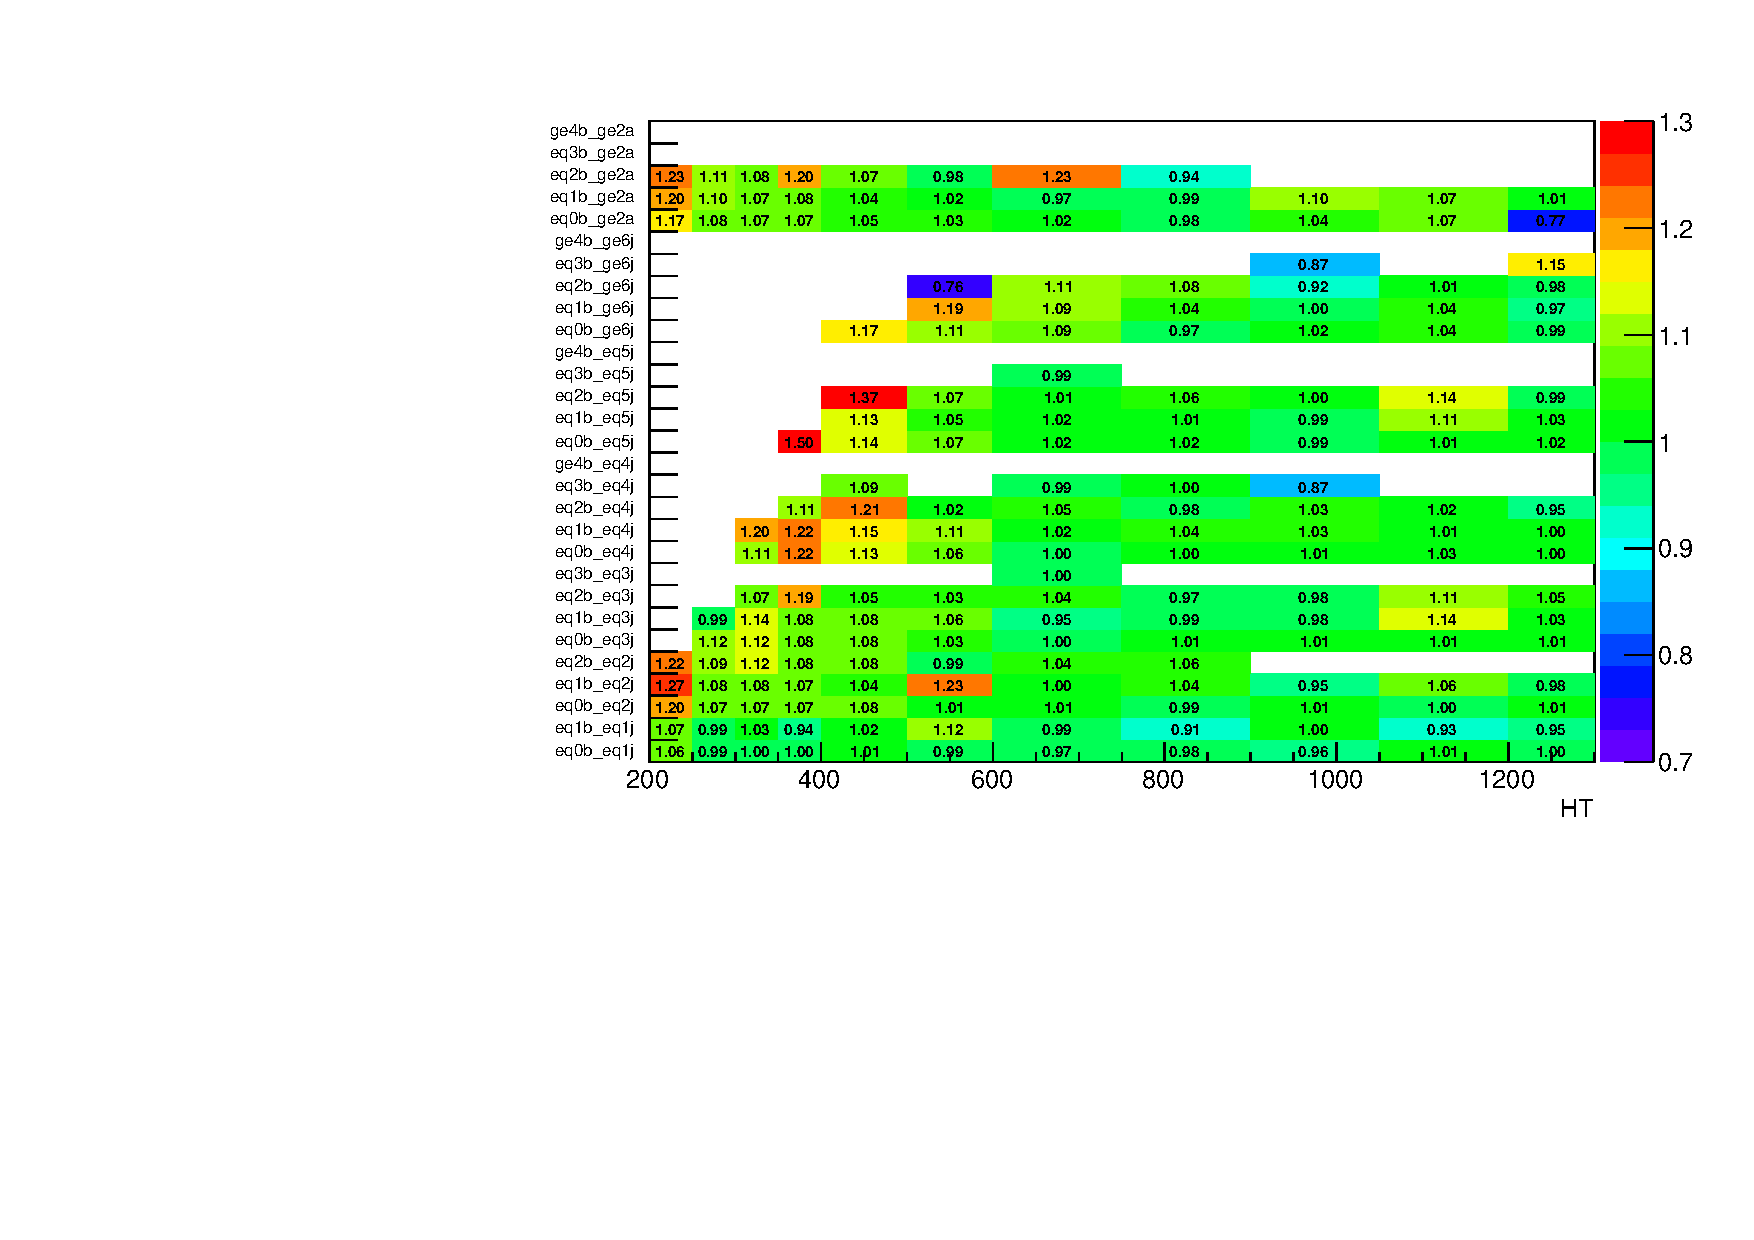
\includegraphics[width=0.5\textwidth]{figures/mcSystematics36p4fb/Zinv/mu/ratiotfh_ht_mht_alljecWeight_Up.pdf}
  } ~~
  \subfigure[JEC down variation]{
    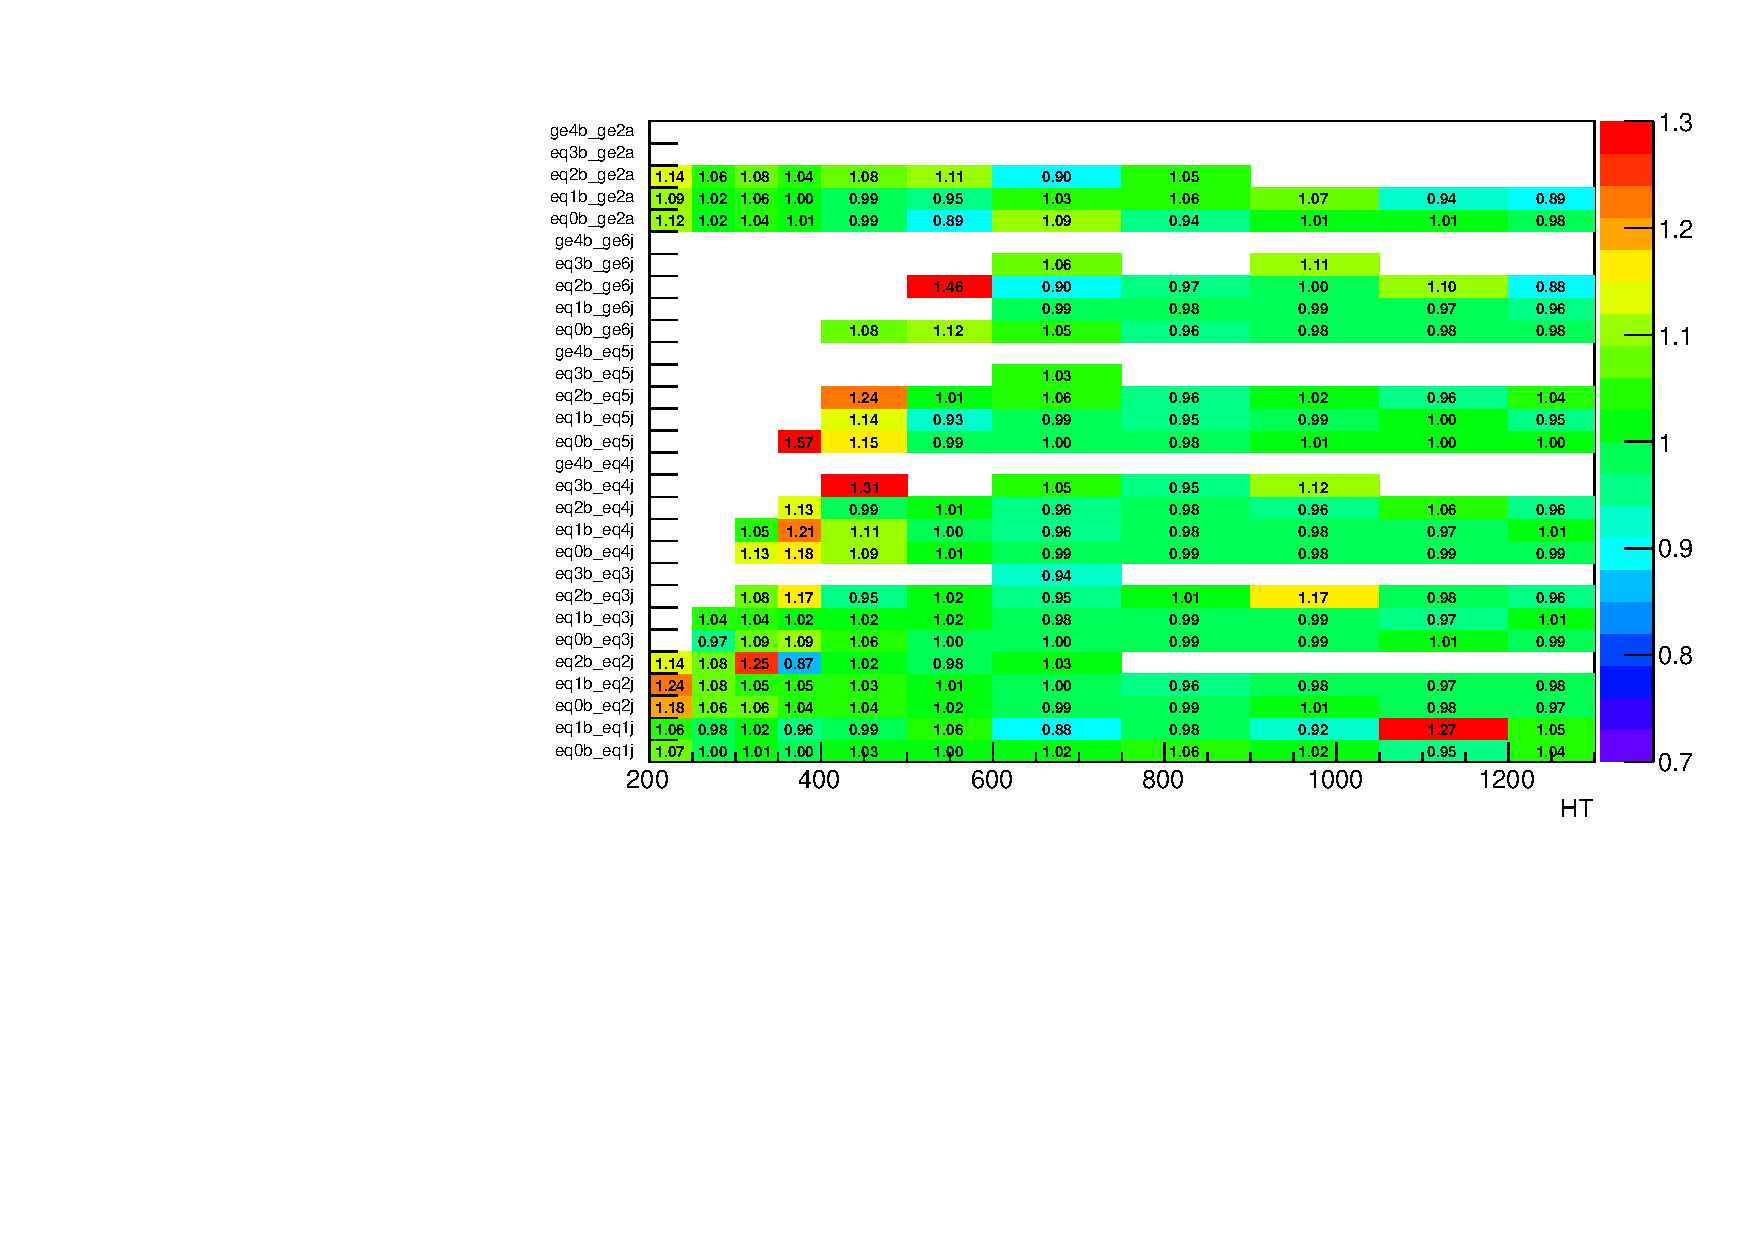
\includegraphics[width=0.5\textwidth]{figures/mcSystematics36p4fb/Zinv/mu/ratiotfh_ht_mht_alljecWeight_Down.pdf}
  }\\

  \caption{\label{fig:tfSyst_jec_muToZinv} The relative change in the
  $\mj \rightarrow (\znunu)$ transfer
  factors when varying JEC in MC within its uncertainties, as a function of \scalht and jet category. 
  Variations corresponding to $+1\sigma$ ($-1\sigma$) are shown in the left (right) figure. 
  }
\end{figure}

\begin{figure}[!h]
  \centering
  \subfigure[JEC up variation]{
    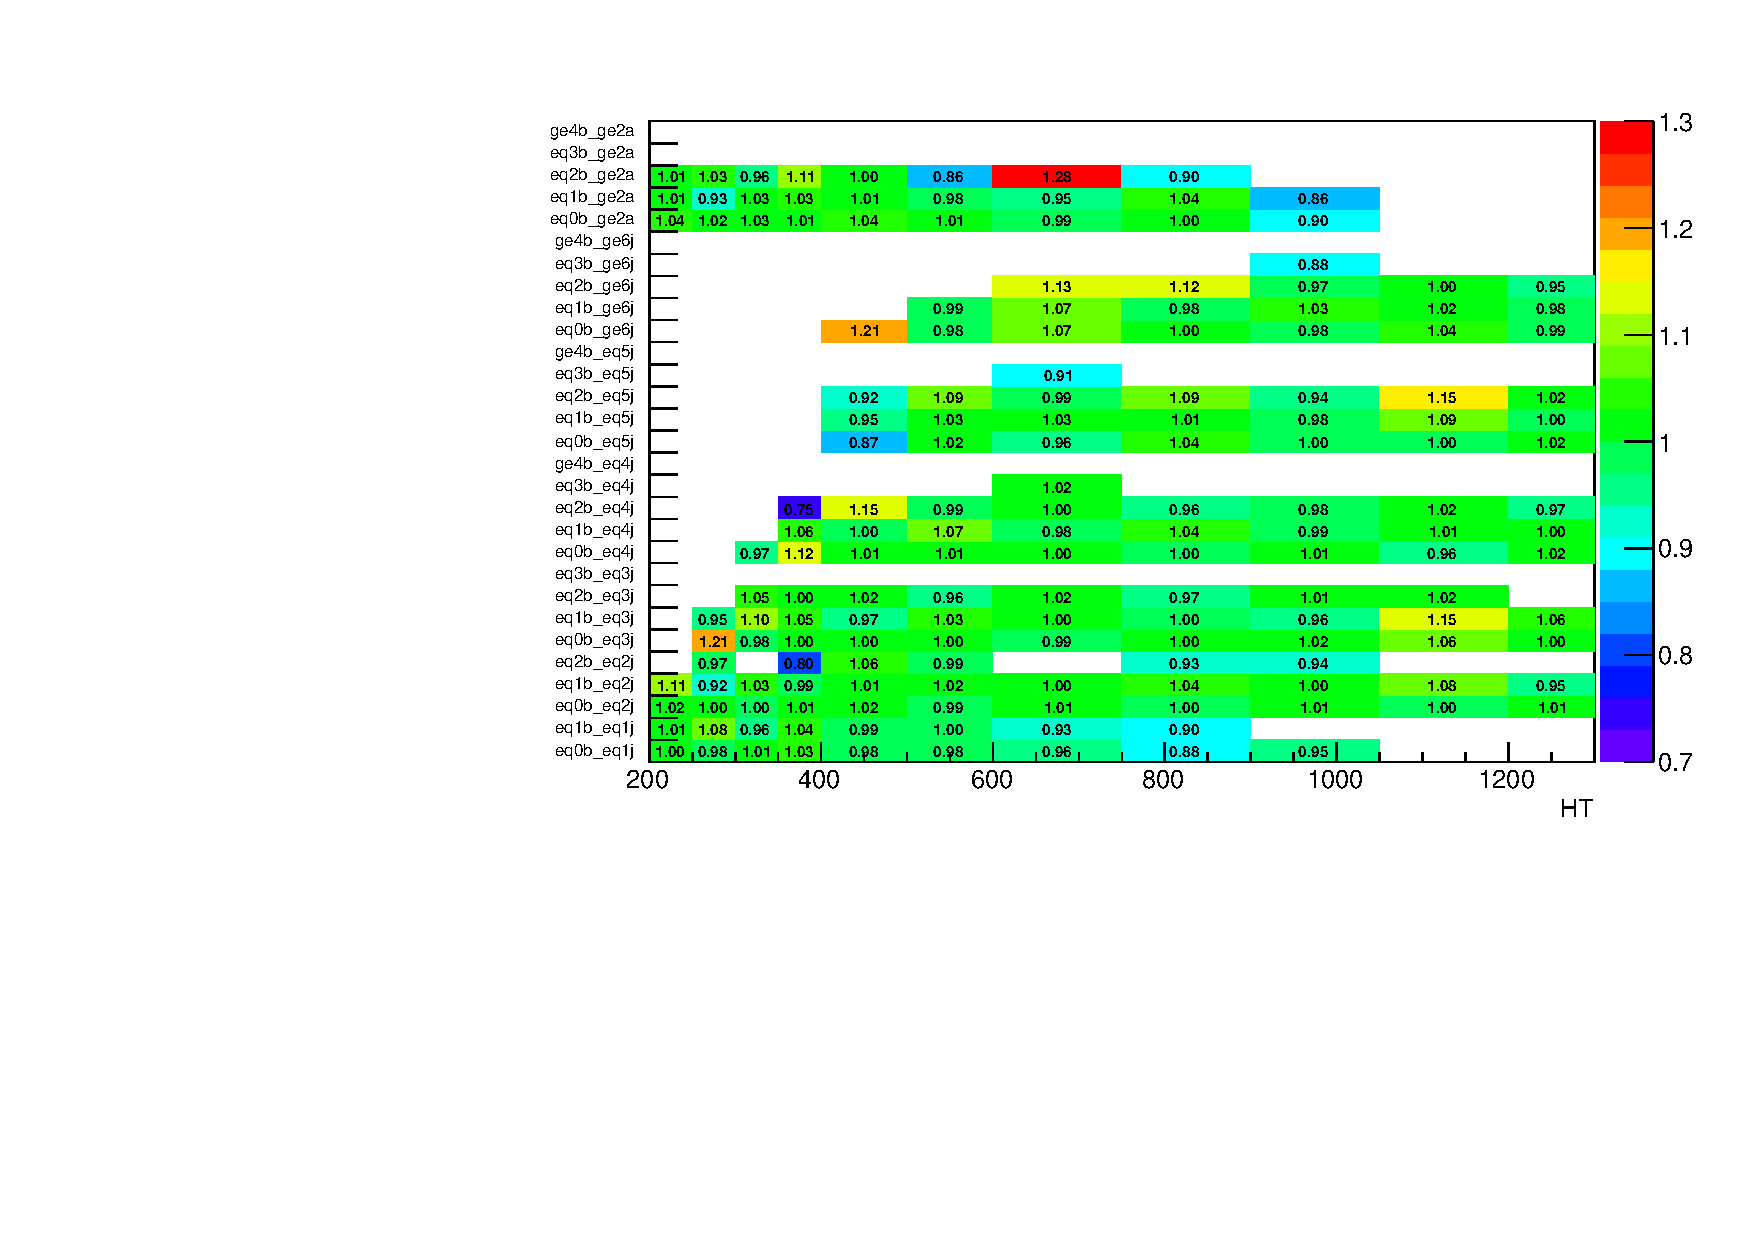
\includegraphics[width=0.5\textwidth]{figures/mcSystematics36p4fb/Zinv/mumu/ratiotfh_ht_mht_alljecWeight_Up.pdf}
  } ~~
  \subfigure[JEC down variation]{
    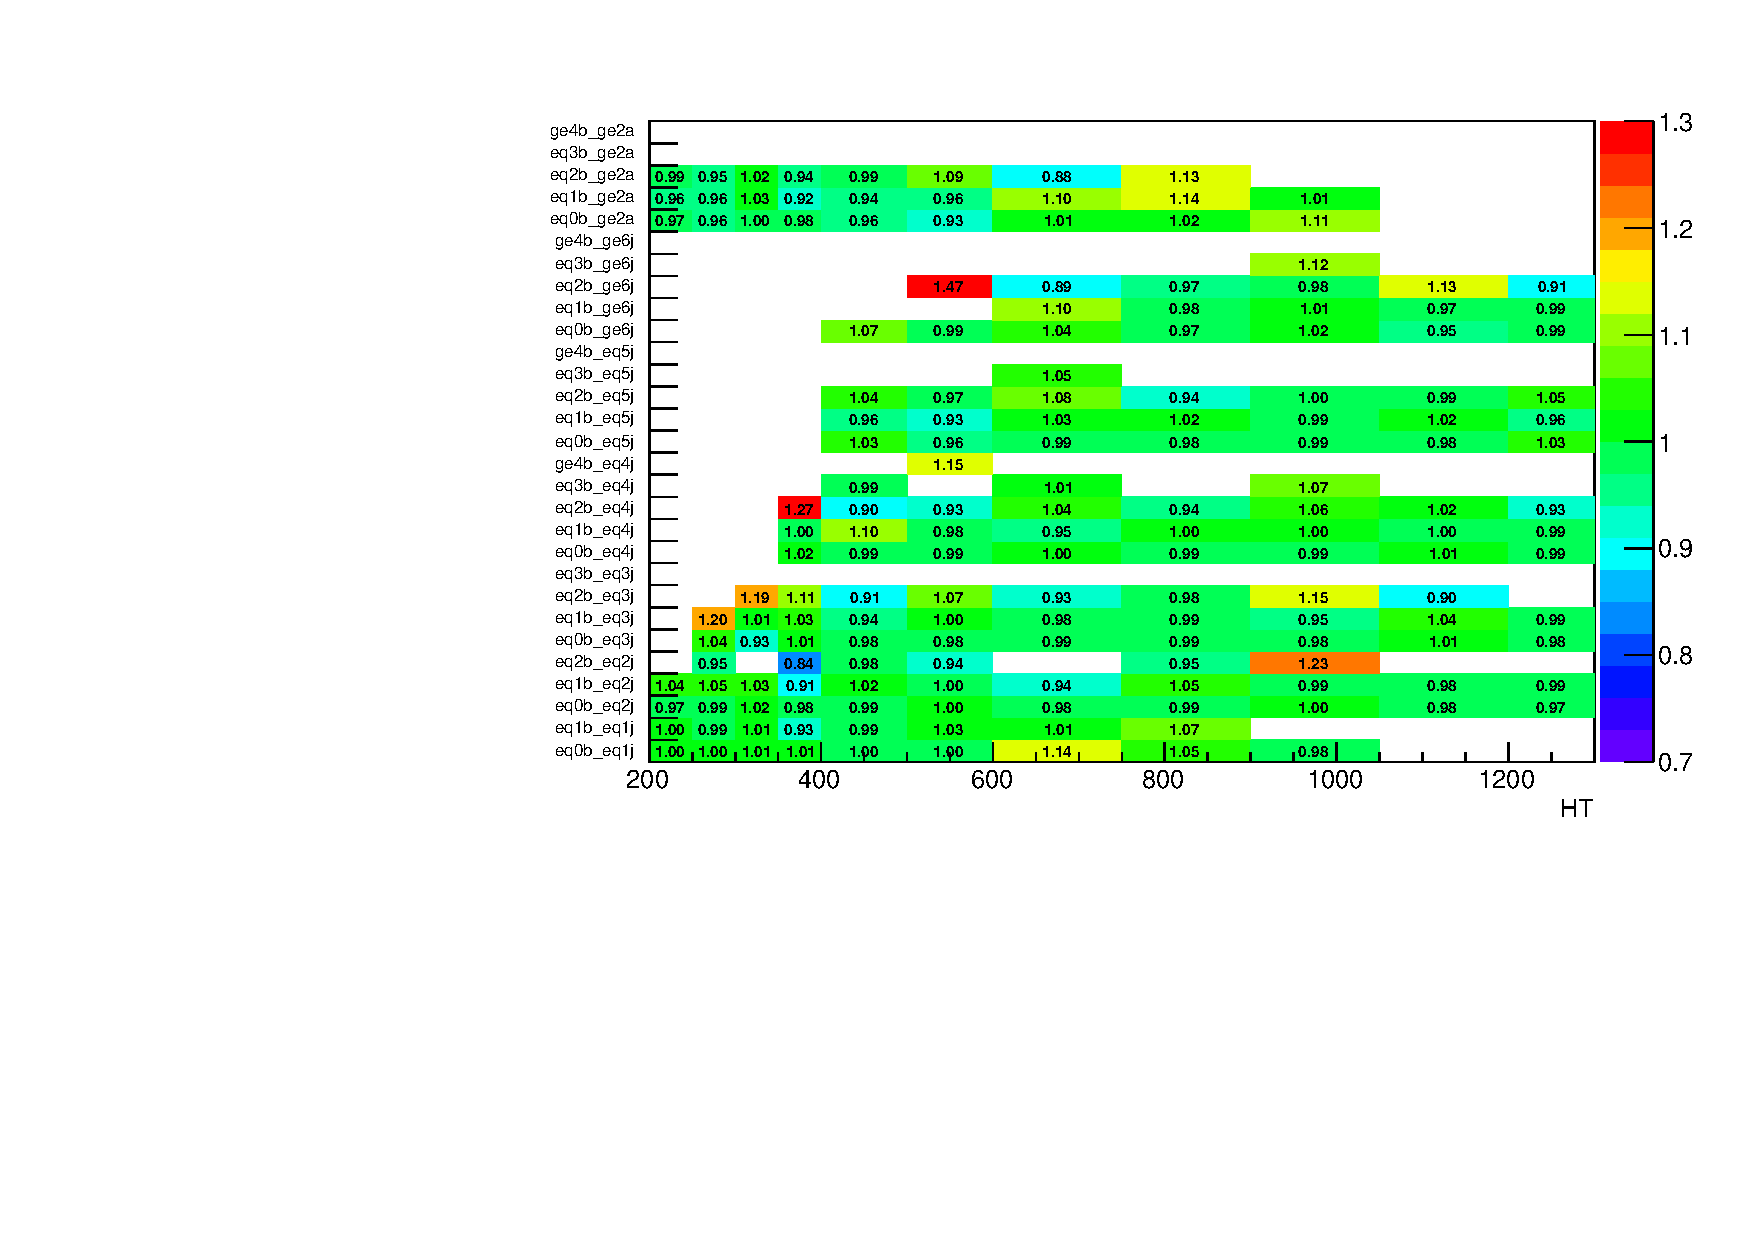
\includegraphics[width=0.5\textwidth]{figures/mcSystematics36p4fb/Zinv/mumu/ratiotfh_ht_mht_alljecWeight_Down.pdf}
  }\\

  \caption{\label{fig:tfSyst_jec_mumuToZinv} The relative change in
  the $\mmj \rightarrow (\znunu)$ transfer
  factors when varying JEC in MC within its uncertainties, as a function of \scalht and jet category. 
  Variations corresponding to $+1\sigma$ ($-1\sigma$) are shown in the left (right) figure. 
  }
\end{figure}

\begin{figure}[!h]
  \centering
  \subfigure[JEC up variation]{
    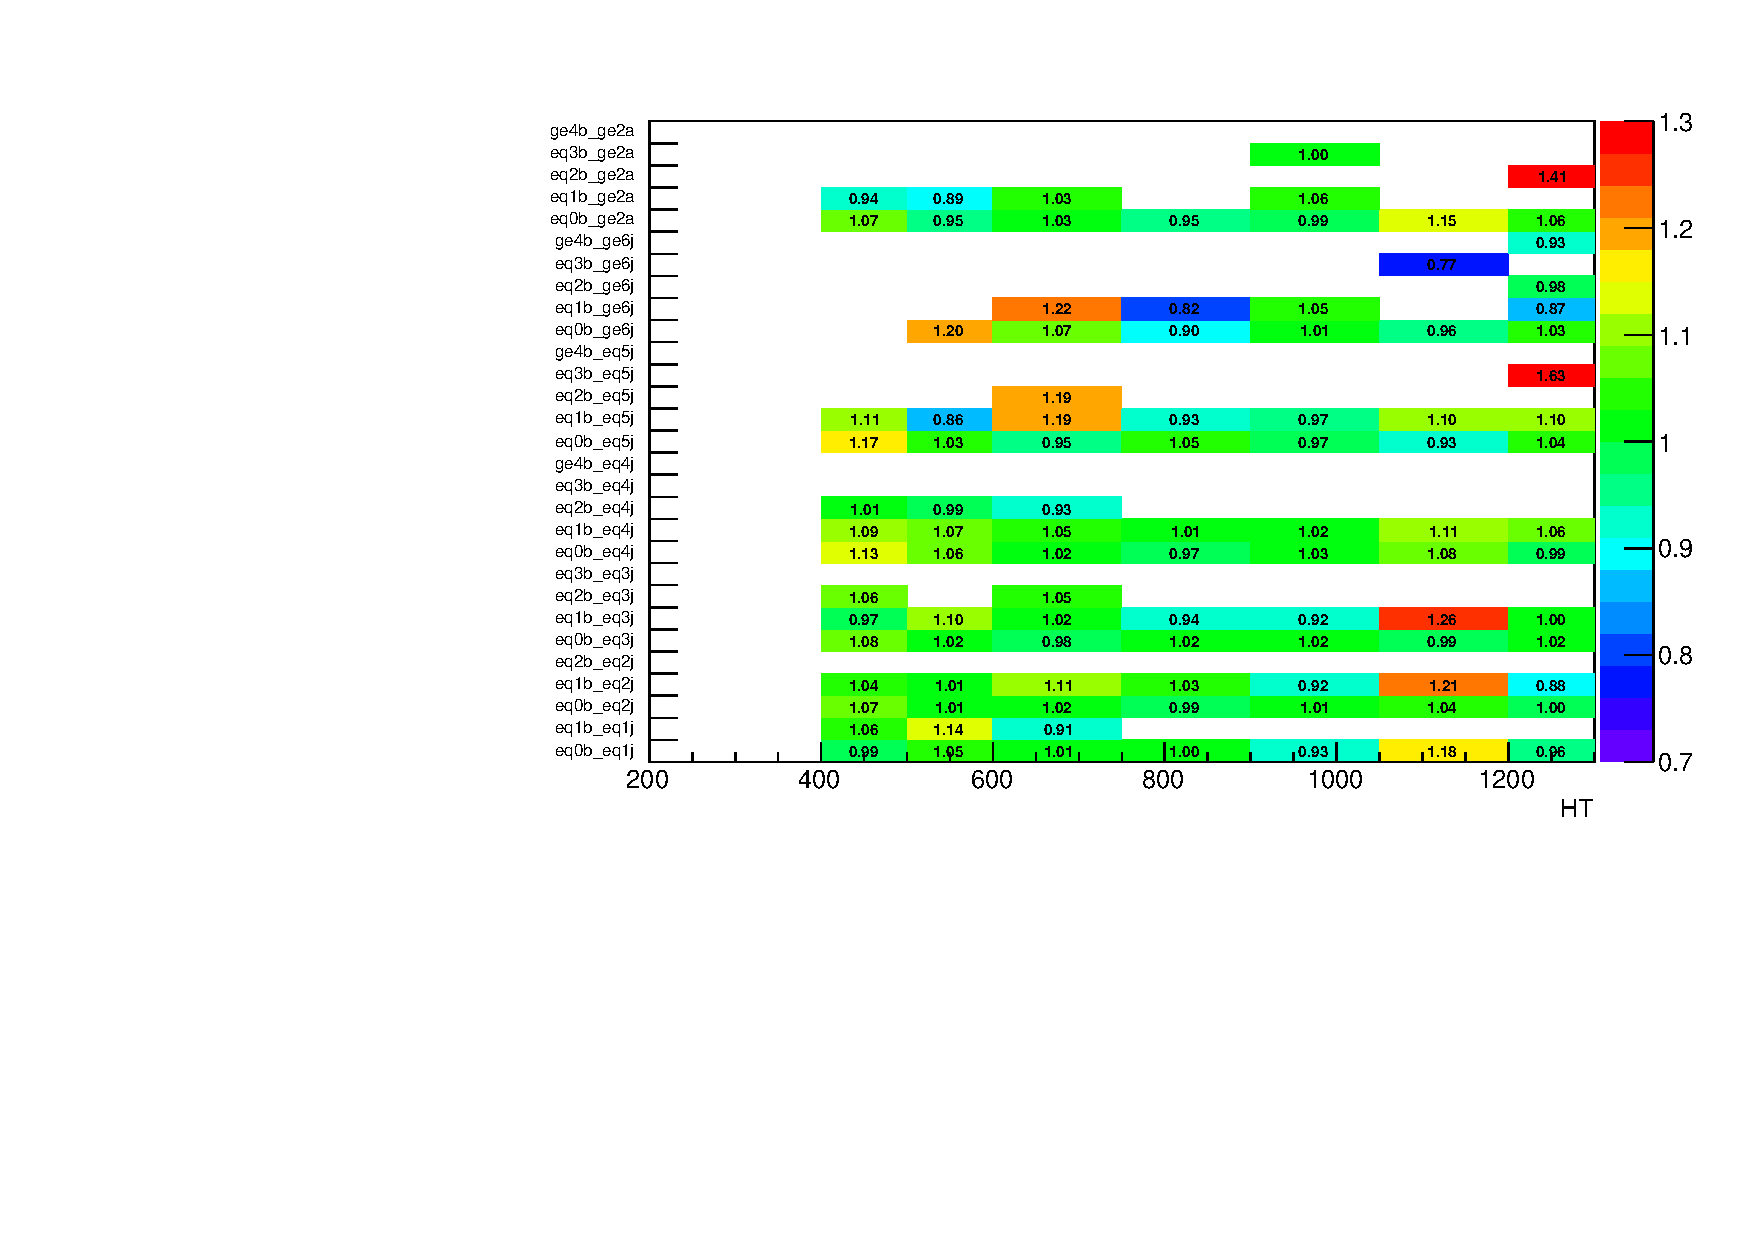
\includegraphics[width=0.5\textwidth]{figures/mcSystematics36p4fb/Zinv/gj/ratiotfh_ht_mht_alljecWeight_Up.pdf}
  } ~~
  \subfigure[JEC down variation]{
    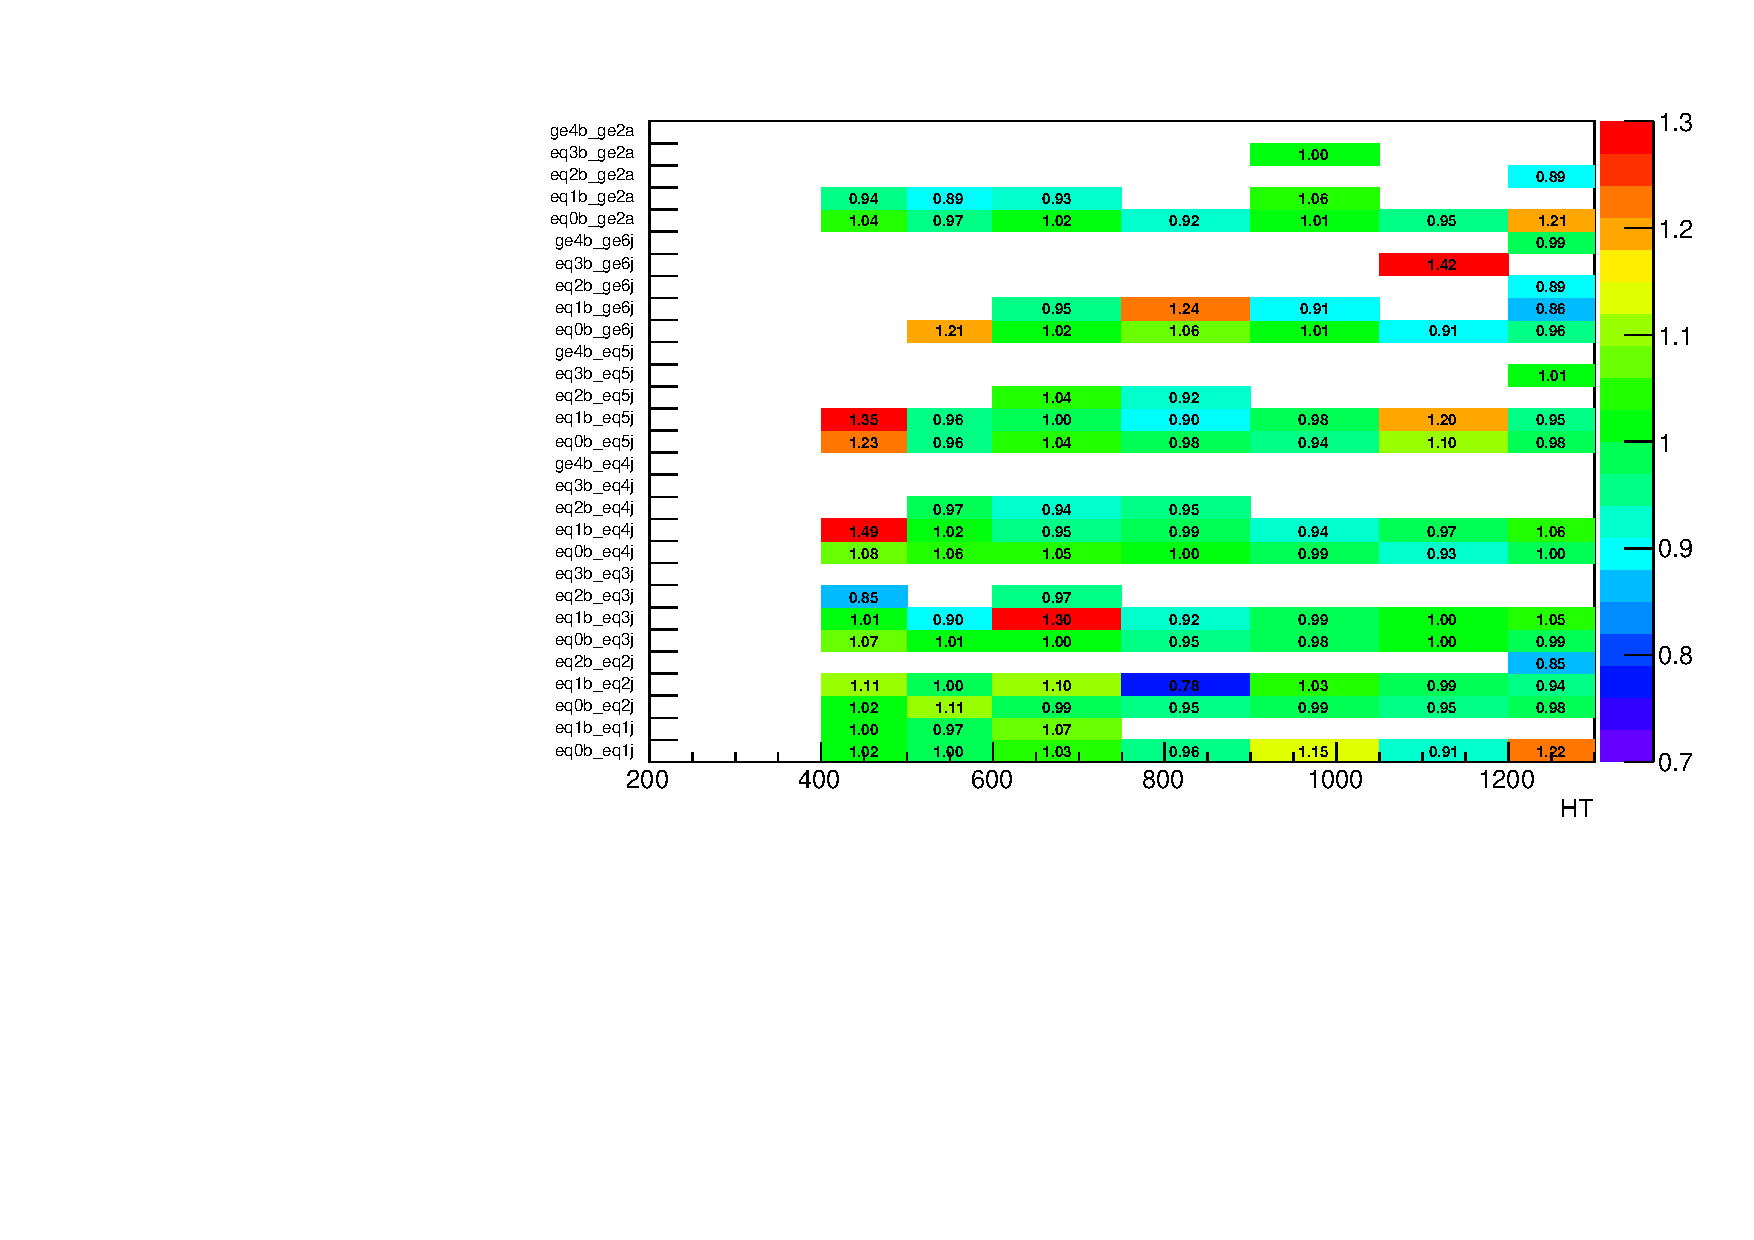
\includegraphics[width=0.5\textwidth]{figures/mcSystematics36p4fb/Zinv/gj/ratiotfh_ht_mht_alljecWeight_Down.pdf}
  }\\

  \caption{\label{fig:tfSyst_jec_gjToZinv} The relative change in the
  $\gj \rightarrow (\znunu)$ transfer
  factors when varying JEC in MC within its uncertainties, as a function of \scalht and jet category. 
  Variations corresponding to $+1\sigma$ ($-1\sigma$) are shown in the left (right) figure. 
  }
\end{figure}

\begin{figure}[!h]
  \centering
  \subfigure[JEC up variation]{
    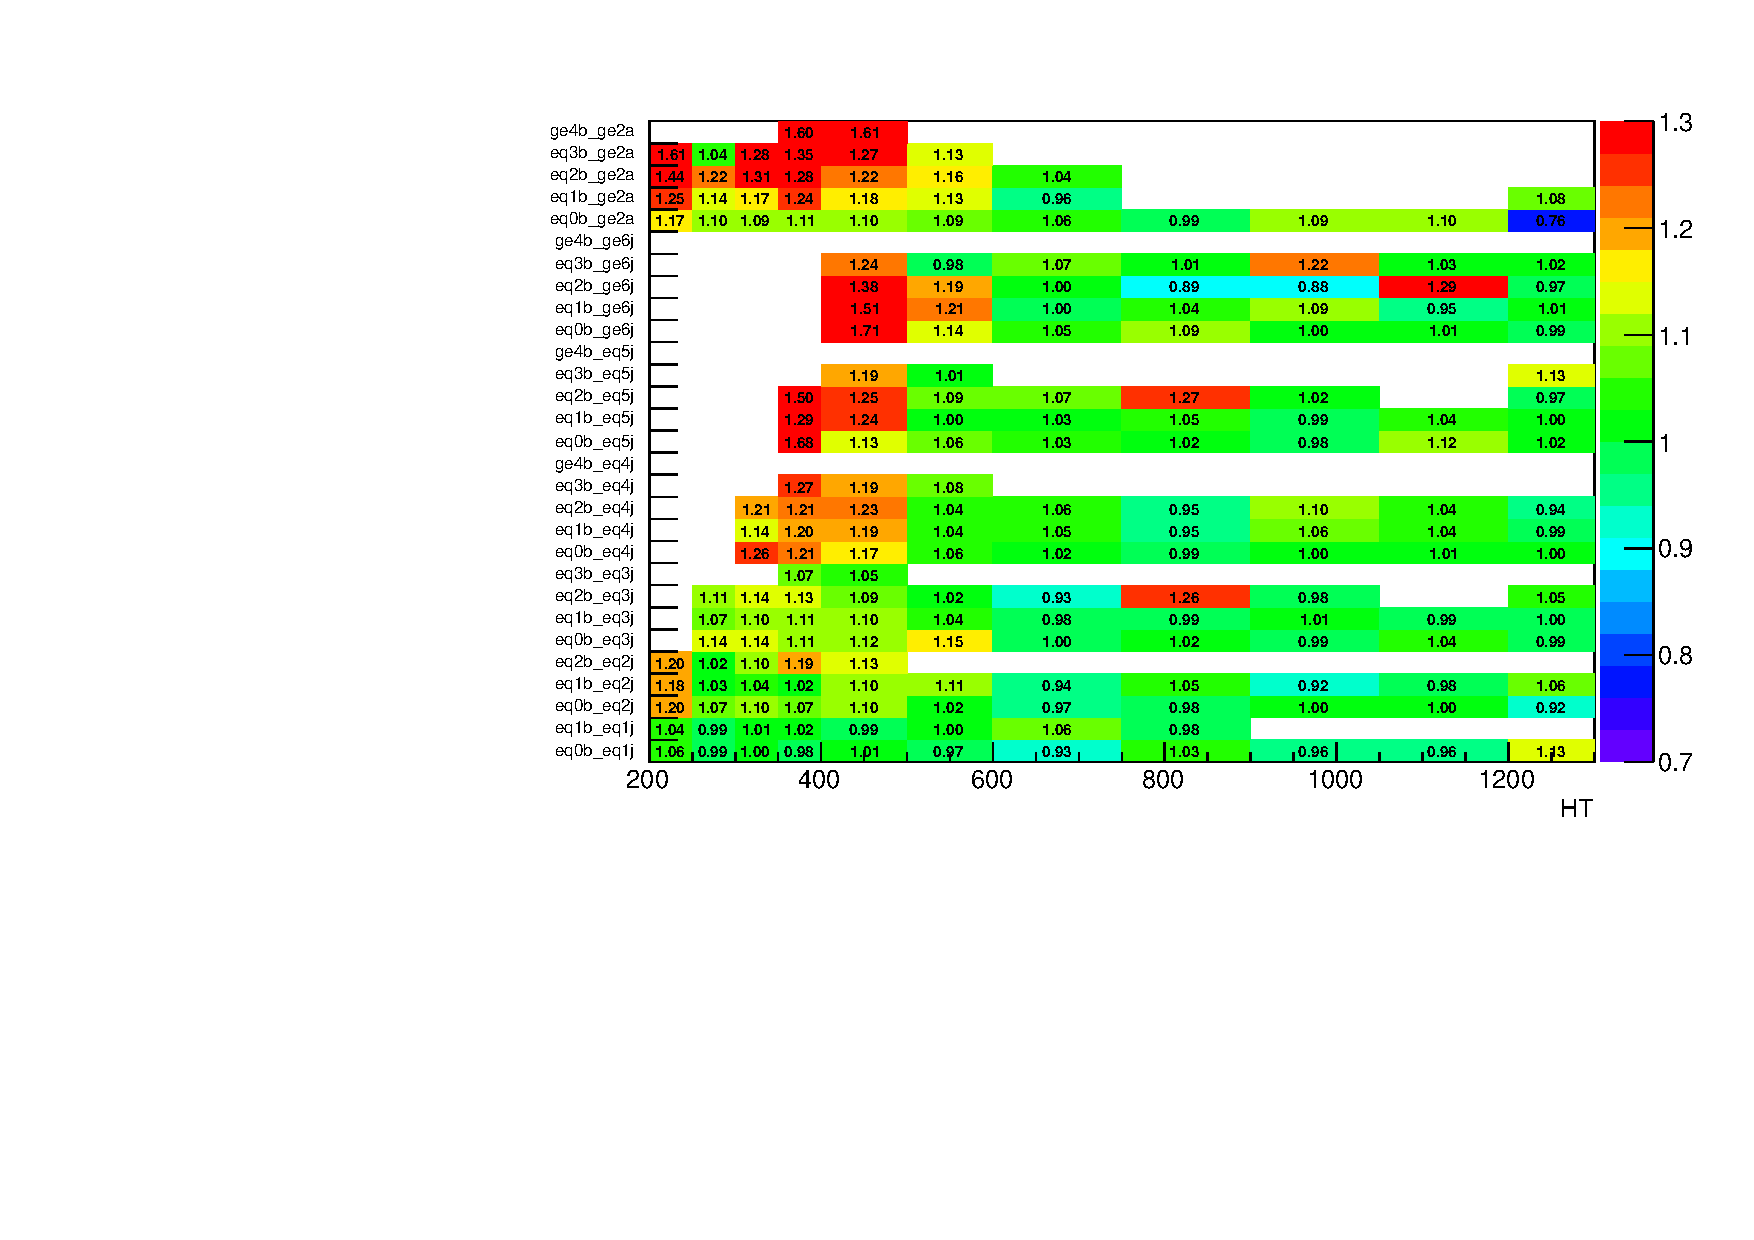
\includegraphics[width=0.5\textwidth]{figures/mcSystematics36p4fb/Ttw/mu/ratiotfh_ht_mht_alljecWeight_Up.pdf}
  } ~~
  \subfigure[JEC down variation]{
    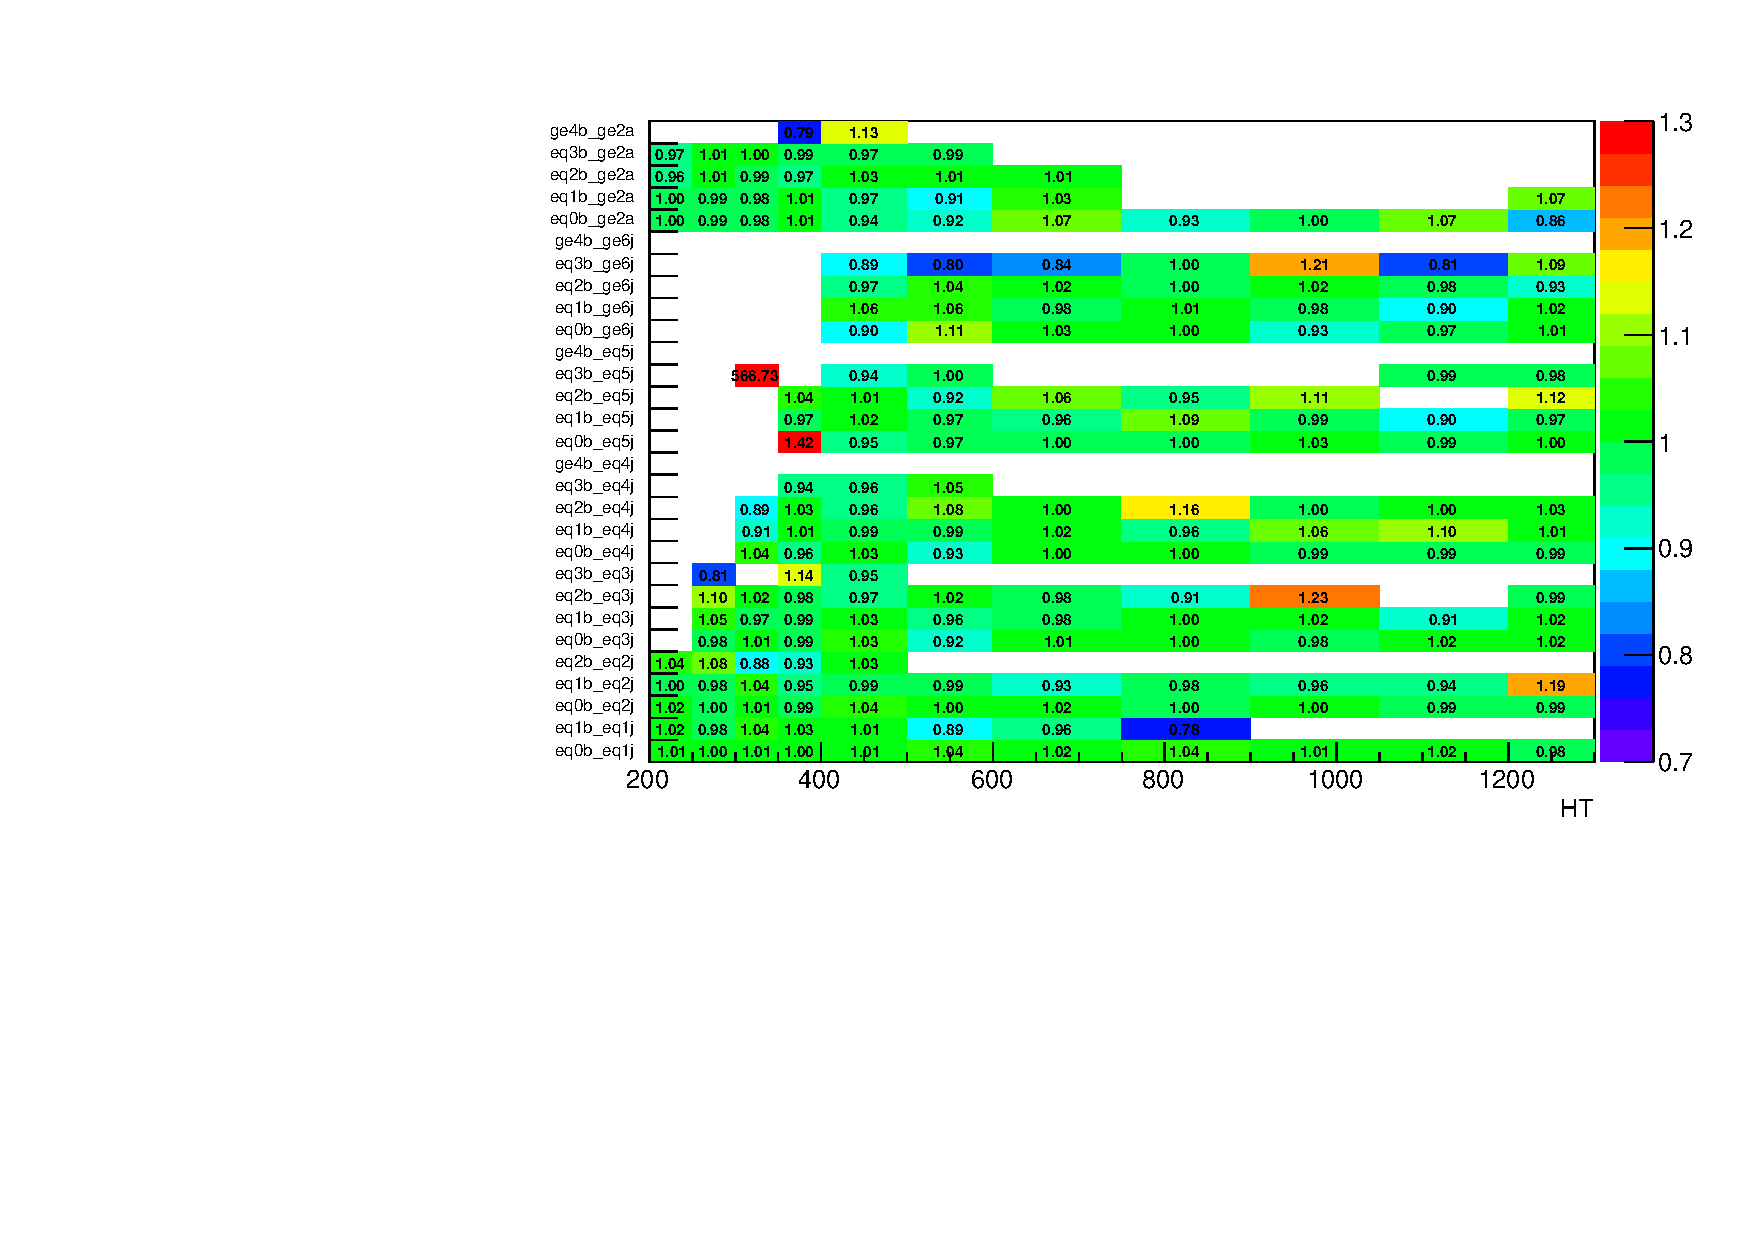
\includegraphics[width=0.5\textwidth]{figures/mcSystematics36p4fb/Ttw/mu/ratiotfh_ht_mht_alljecWeight_Down.pdf}
  }\\

  \caption{\label{fig:tfSyst_jec_muToTtw} The relative change in the
  $\mj \rightarrow \mathrm{\ttbar+W}$ transfer
  factors when varying JEC in MC within its uncertainties, as a function of \scalht and jet category. 
  Variations corresponding to $+1\sigma$ ($-1\sigma$) are shown in the left (right) figure. 
  }
\end{figure}

\clearpage
\subsection{B-tagging efficiency}

\begin{figure}[!h]
  \centering
  \subfigure[b-tag SF (heavy) up variation]{
    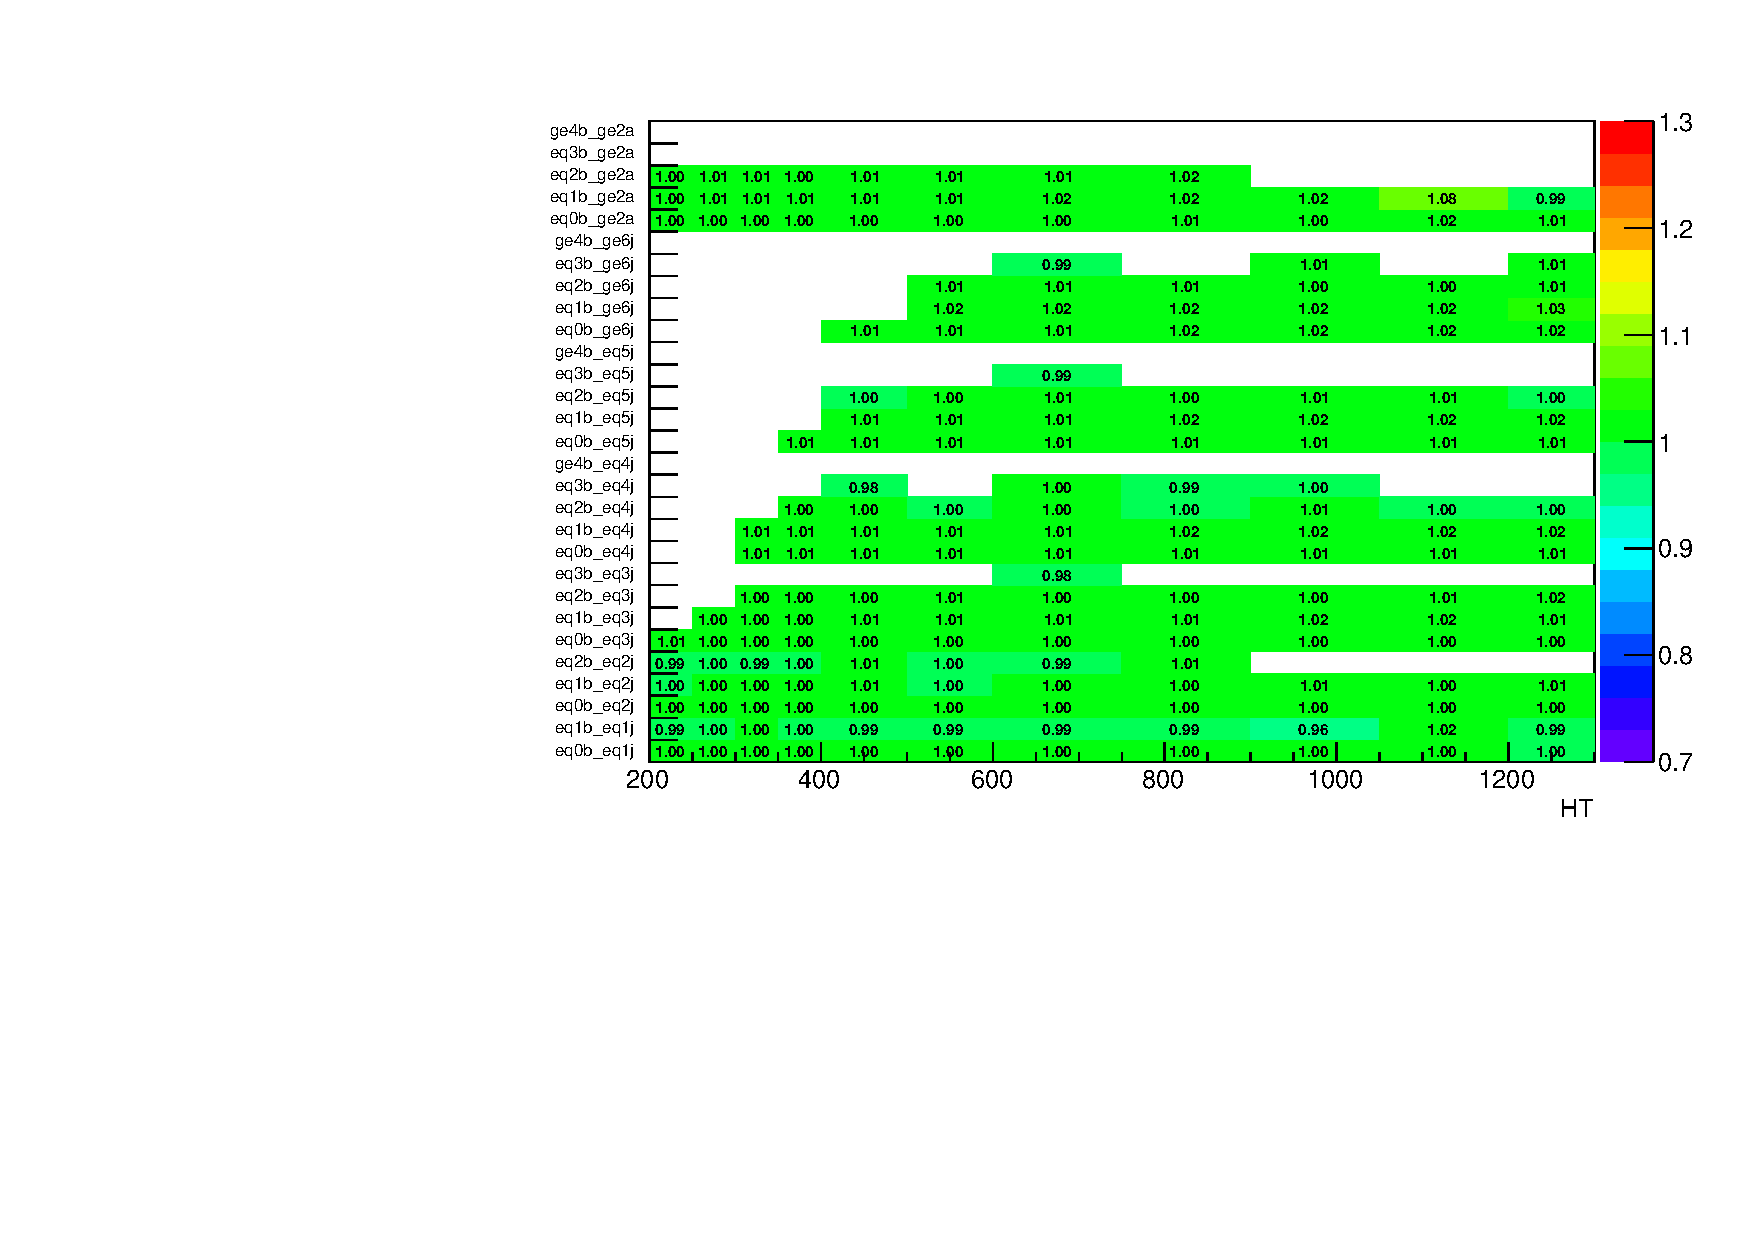
\includegraphics[width=0.5\textwidth]{figures/mcSystematics36p4fb/Zinv/mu/ratiotfh_ht_mht_allbsfWeight_Up.pdf}
  } ~~
  \subfigure[b-tag SF (heavy) down variation]{
    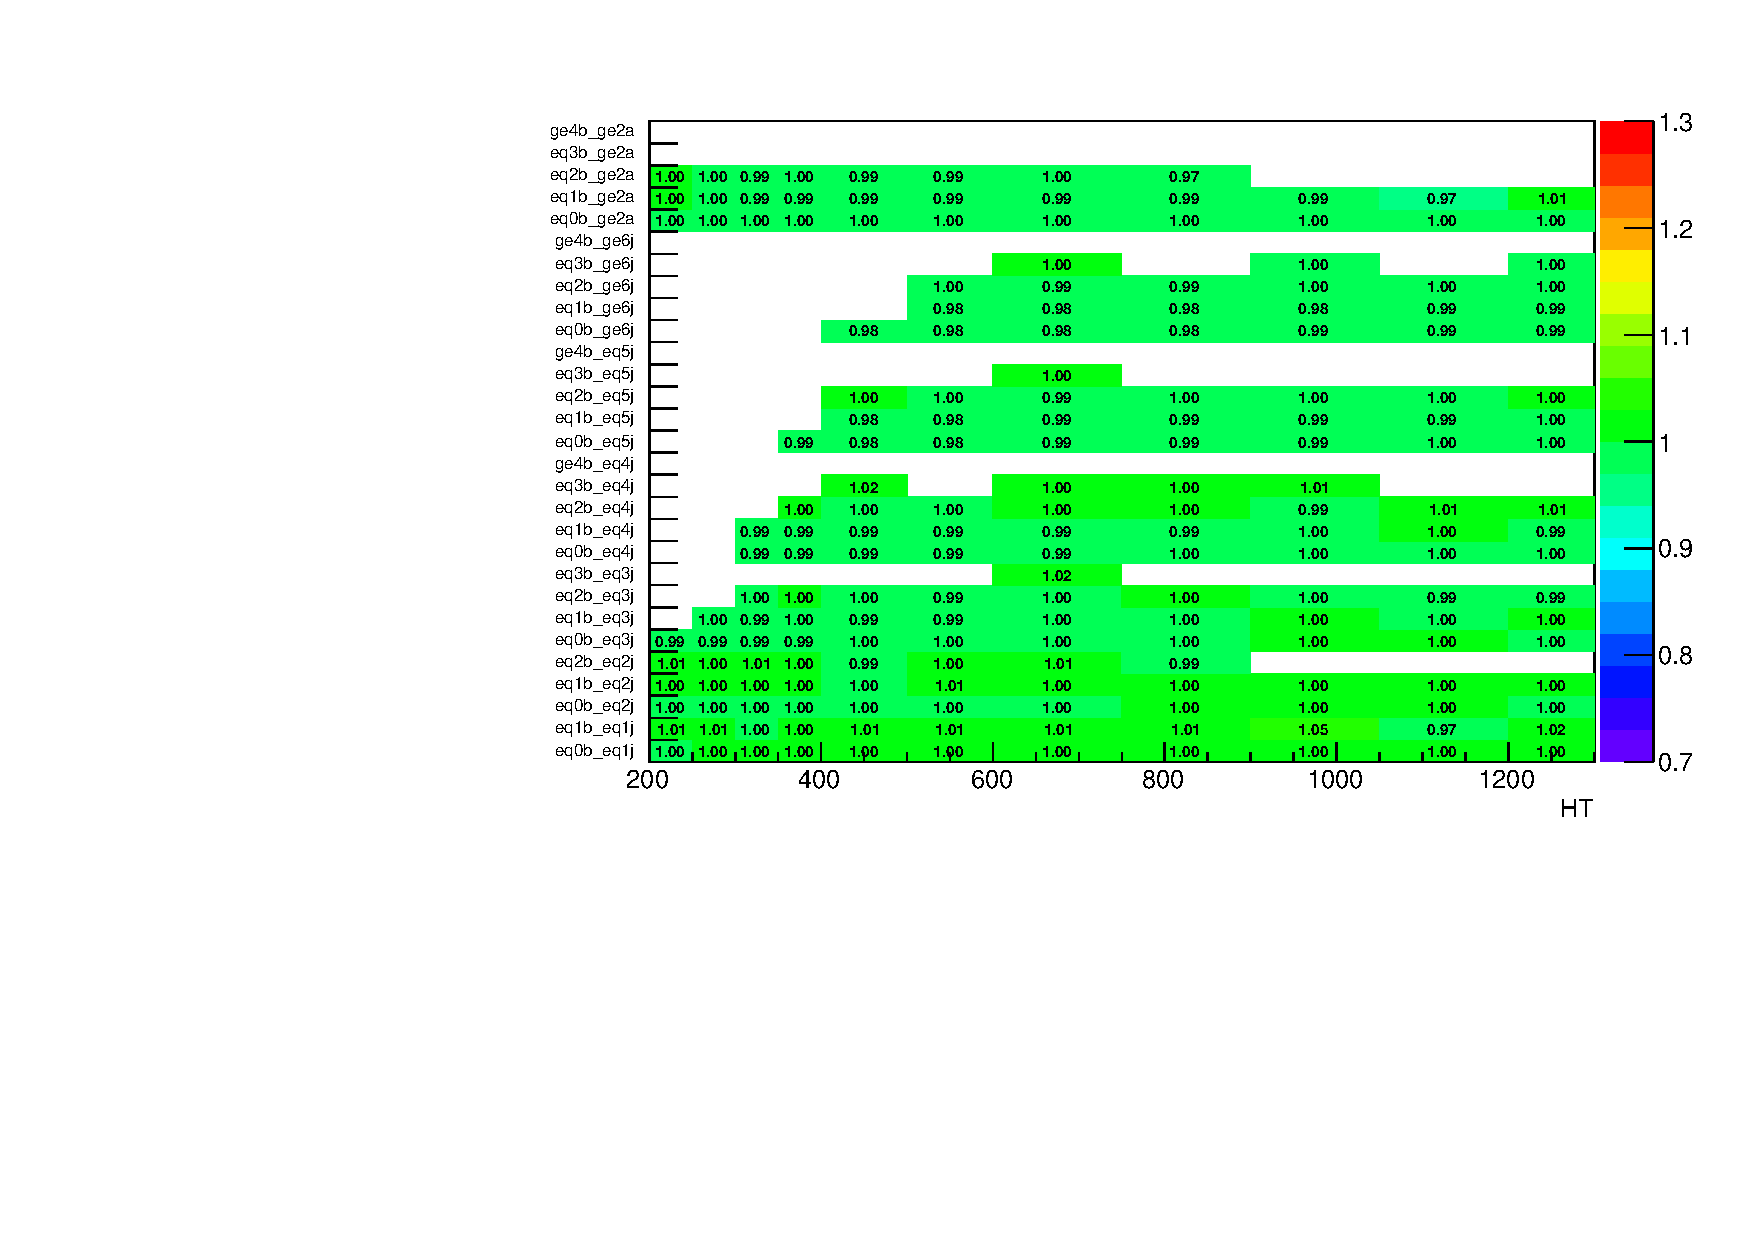
\includegraphics[width=0.5\textwidth]{figures/mcSystematics36p4fb/Zinv/mu/ratiotfh_ht_mht_allbsfWeight_Down.pdf}
  }\\

  \caption{\label{fig:tfSyst_bsf_muToZinv} The relative change in the
  $\mj \rightarrow (\znunu)$ transfer
  factors when varying b-tag SF for heavy jets in MC within its uncertainties, as a function of \scalht and jet category. 
  Variations corresponding to $+1\sigma$ ($-1\sigma$) are shown in the left (right) figure. 
  }
\end{figure}

\begin{figure}[!h]
  \centering
  \subfigure[b-tag SF (heavy) up variation]{
    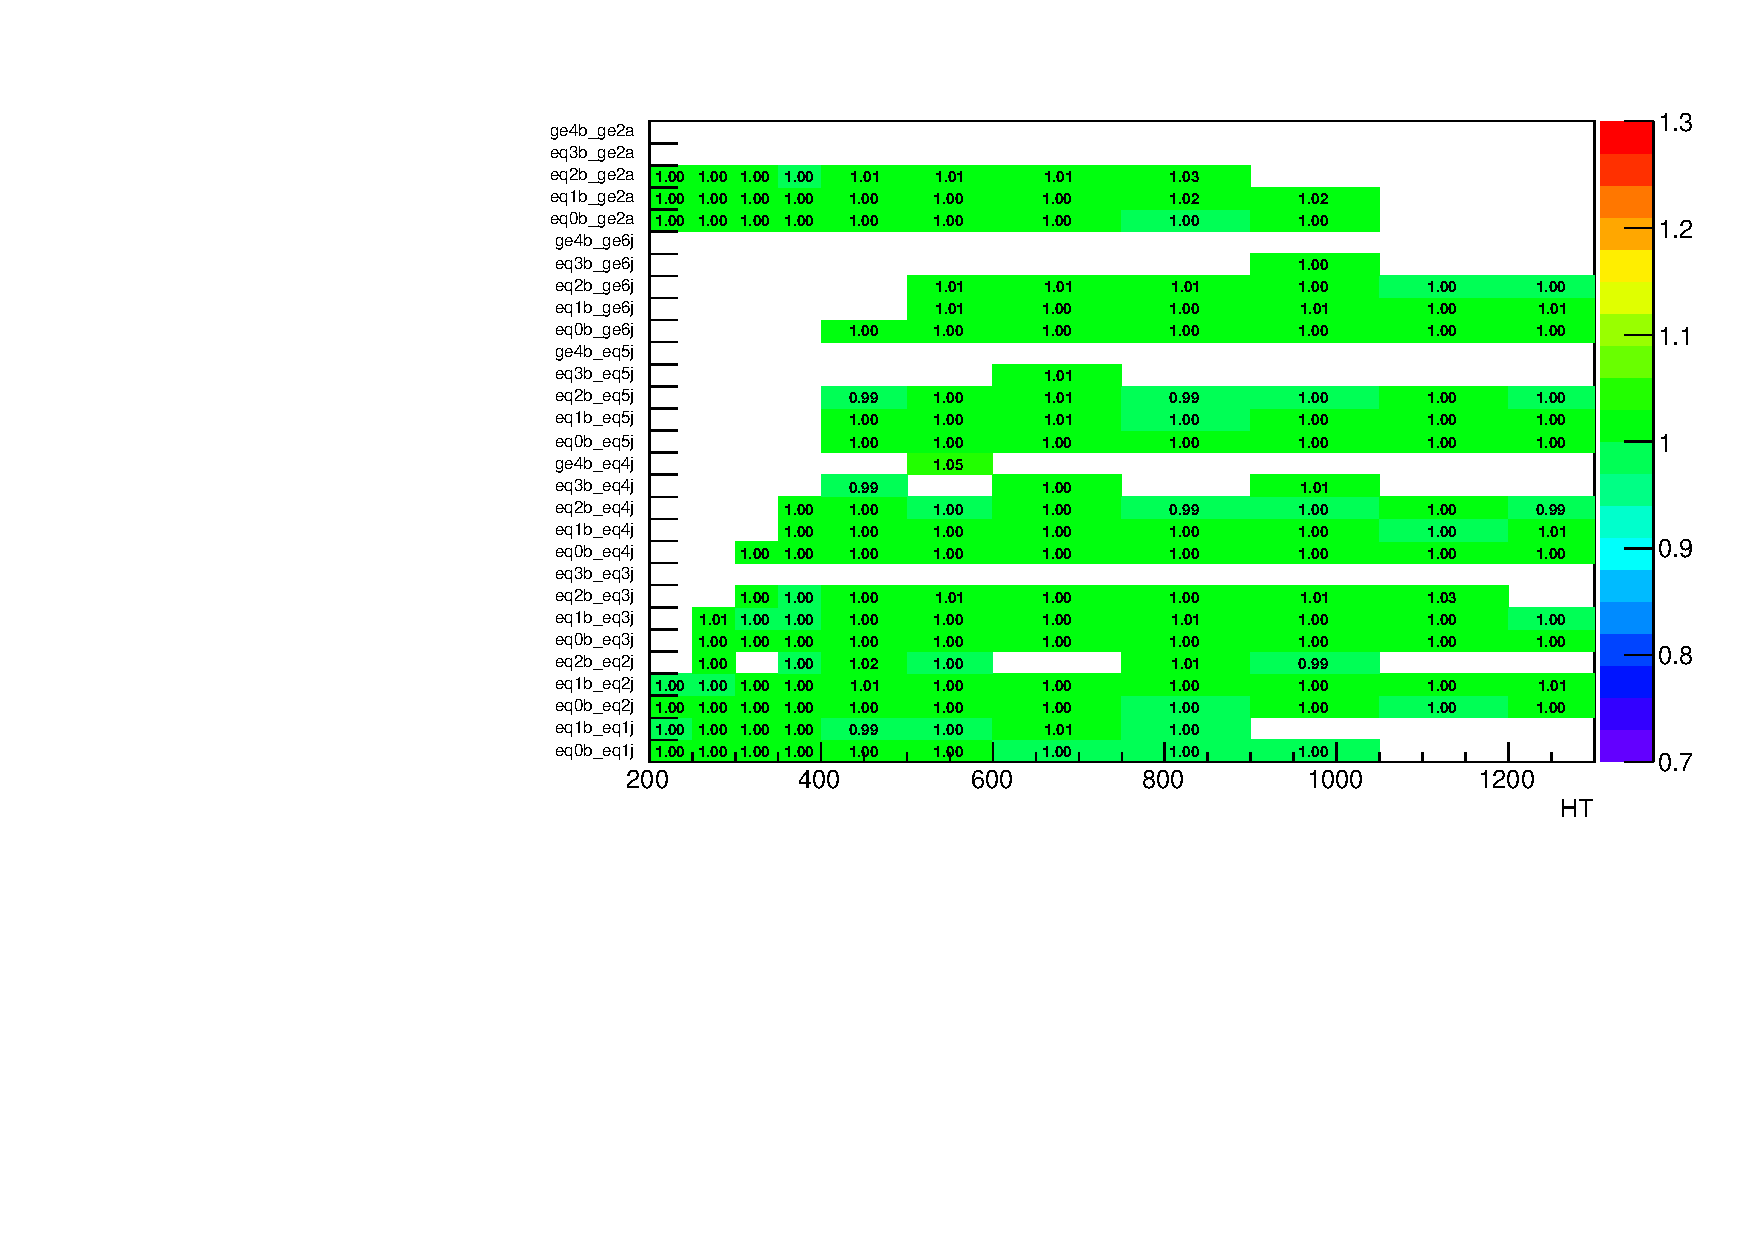
\includegraphics[width=0.5\textwidth]{figures/mcSystematics36p4fb/Zinv/mumu/ratiotfh_ht_mht_allbsfWeight_Up.pdf}
  } ~~
  \subfigure[b-tag SF (heavy) down variation]{
    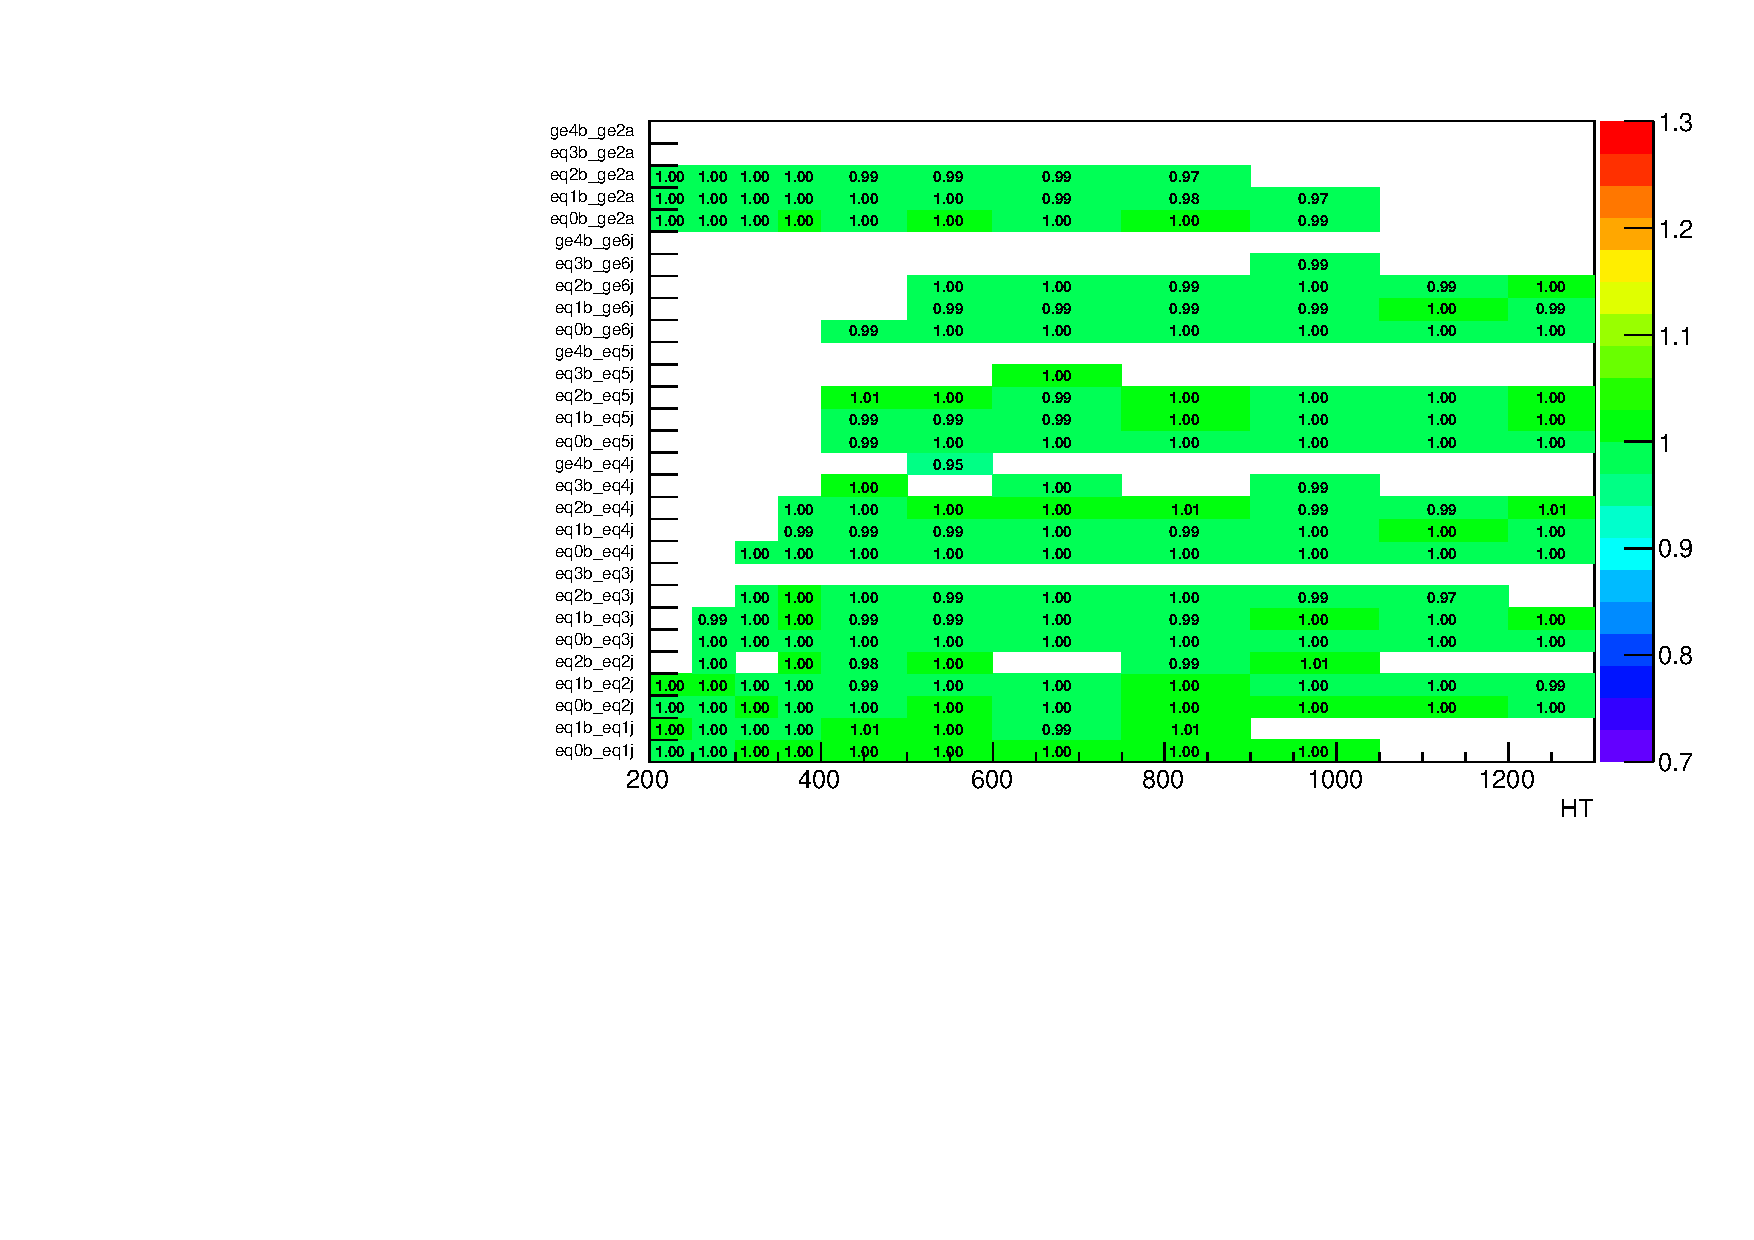
\includegraphics[width=0.5\textwidth]{figures/mcSystematics36p4fb/Zinv/mumu/ratiotfh_ht_mht_allbsfWeight_Down.pdf}
  }\\

  \caption{\label{fig:tfSyst_bsf_mumuToZinv} The relative change in
  the $\mmj \rightarrow (\znunu)$ transfer
  factors when varying b-tag SF for heavy jets in MC within its uncertainties, as a function of \scalht and jet category. 
  Variations corresponding to $+1\sigma$ ($-1\sigma$) are shown in the left (right) figure. 
  }
\end{figure}

\begin{figure}[!h]
  \centering
  \subfigure[b-tag SF (heavy) up variation]{
    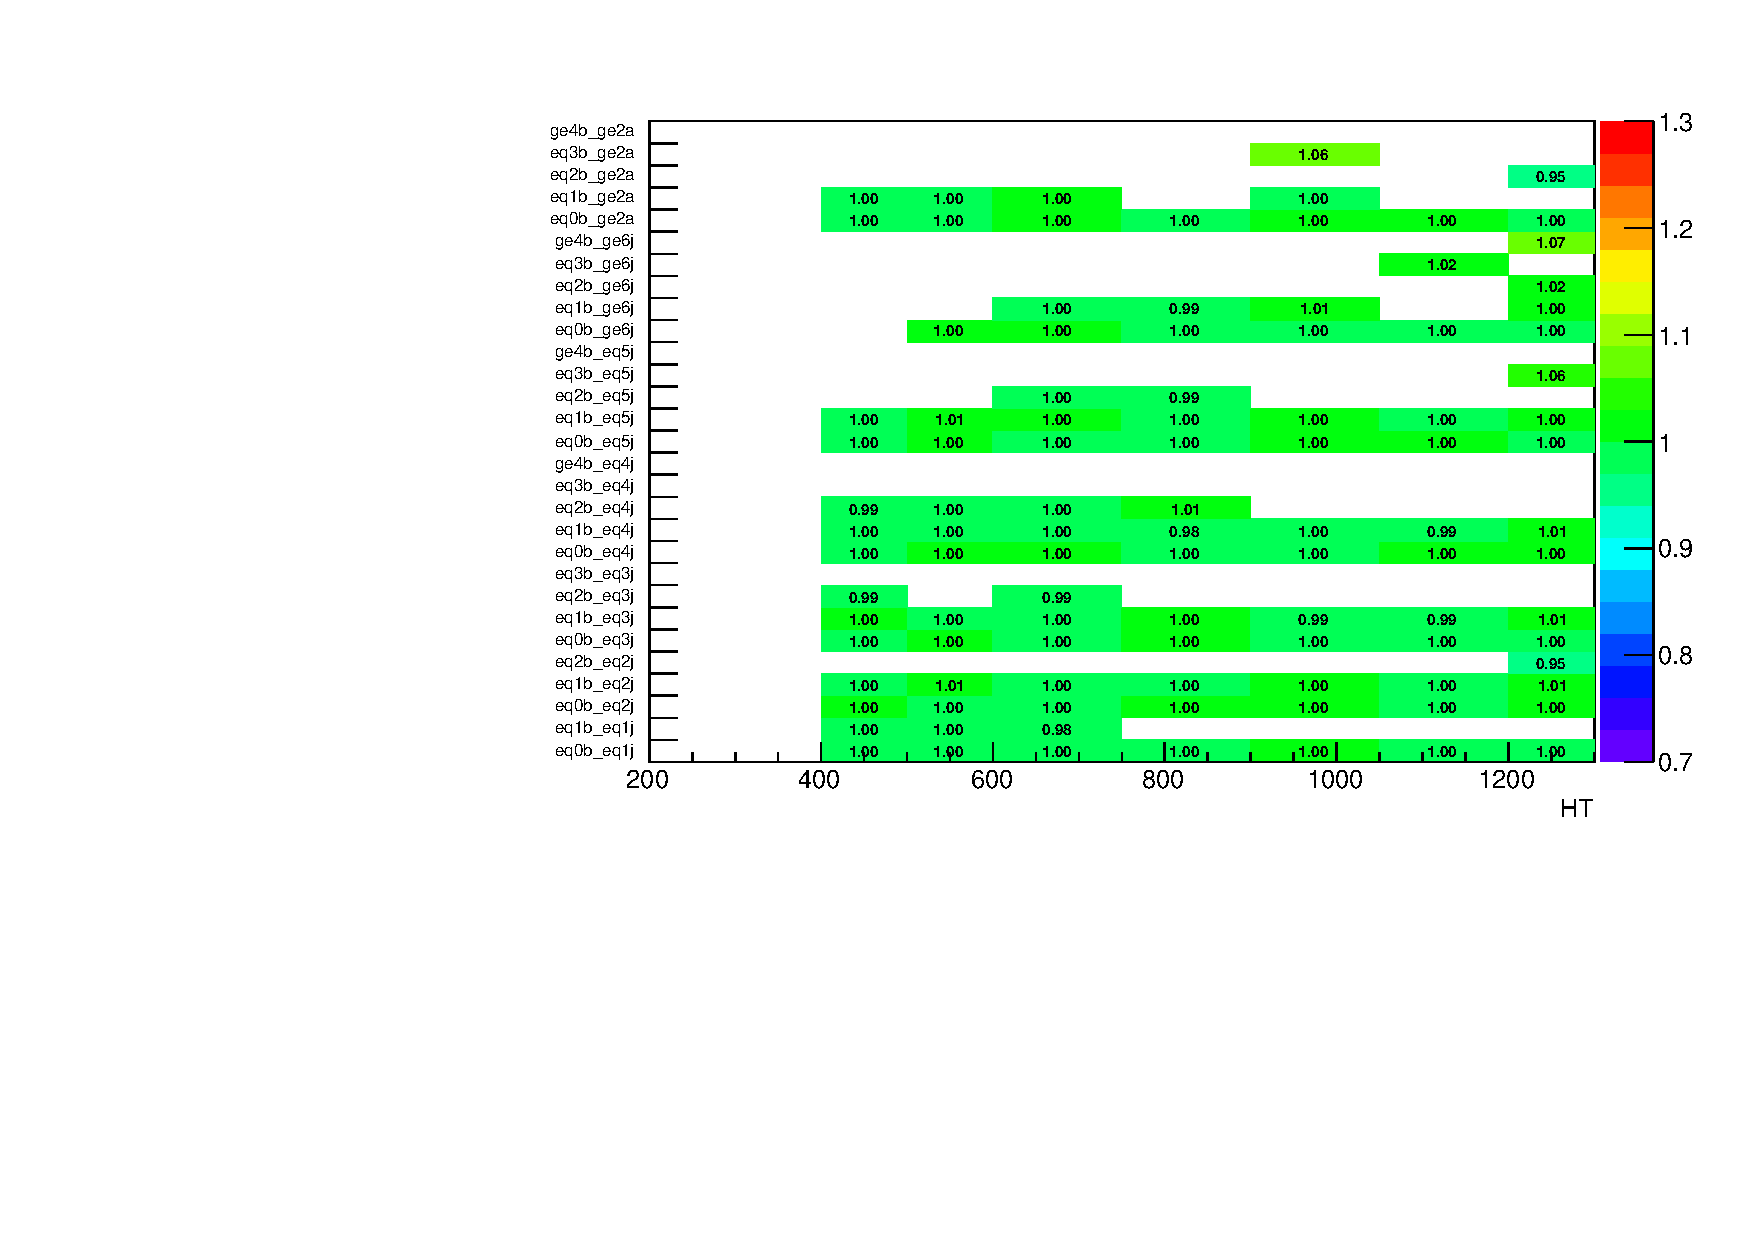
\includegraphics[width=0.5\textwidth]{figures/mcSystematics36p4fb/Zinv/gj/ratiotfh_ht_mht_allbsfWeight_Up.pdf}
  } ~~
  \subfigure[b-tag SF (heavy) down variation]{
    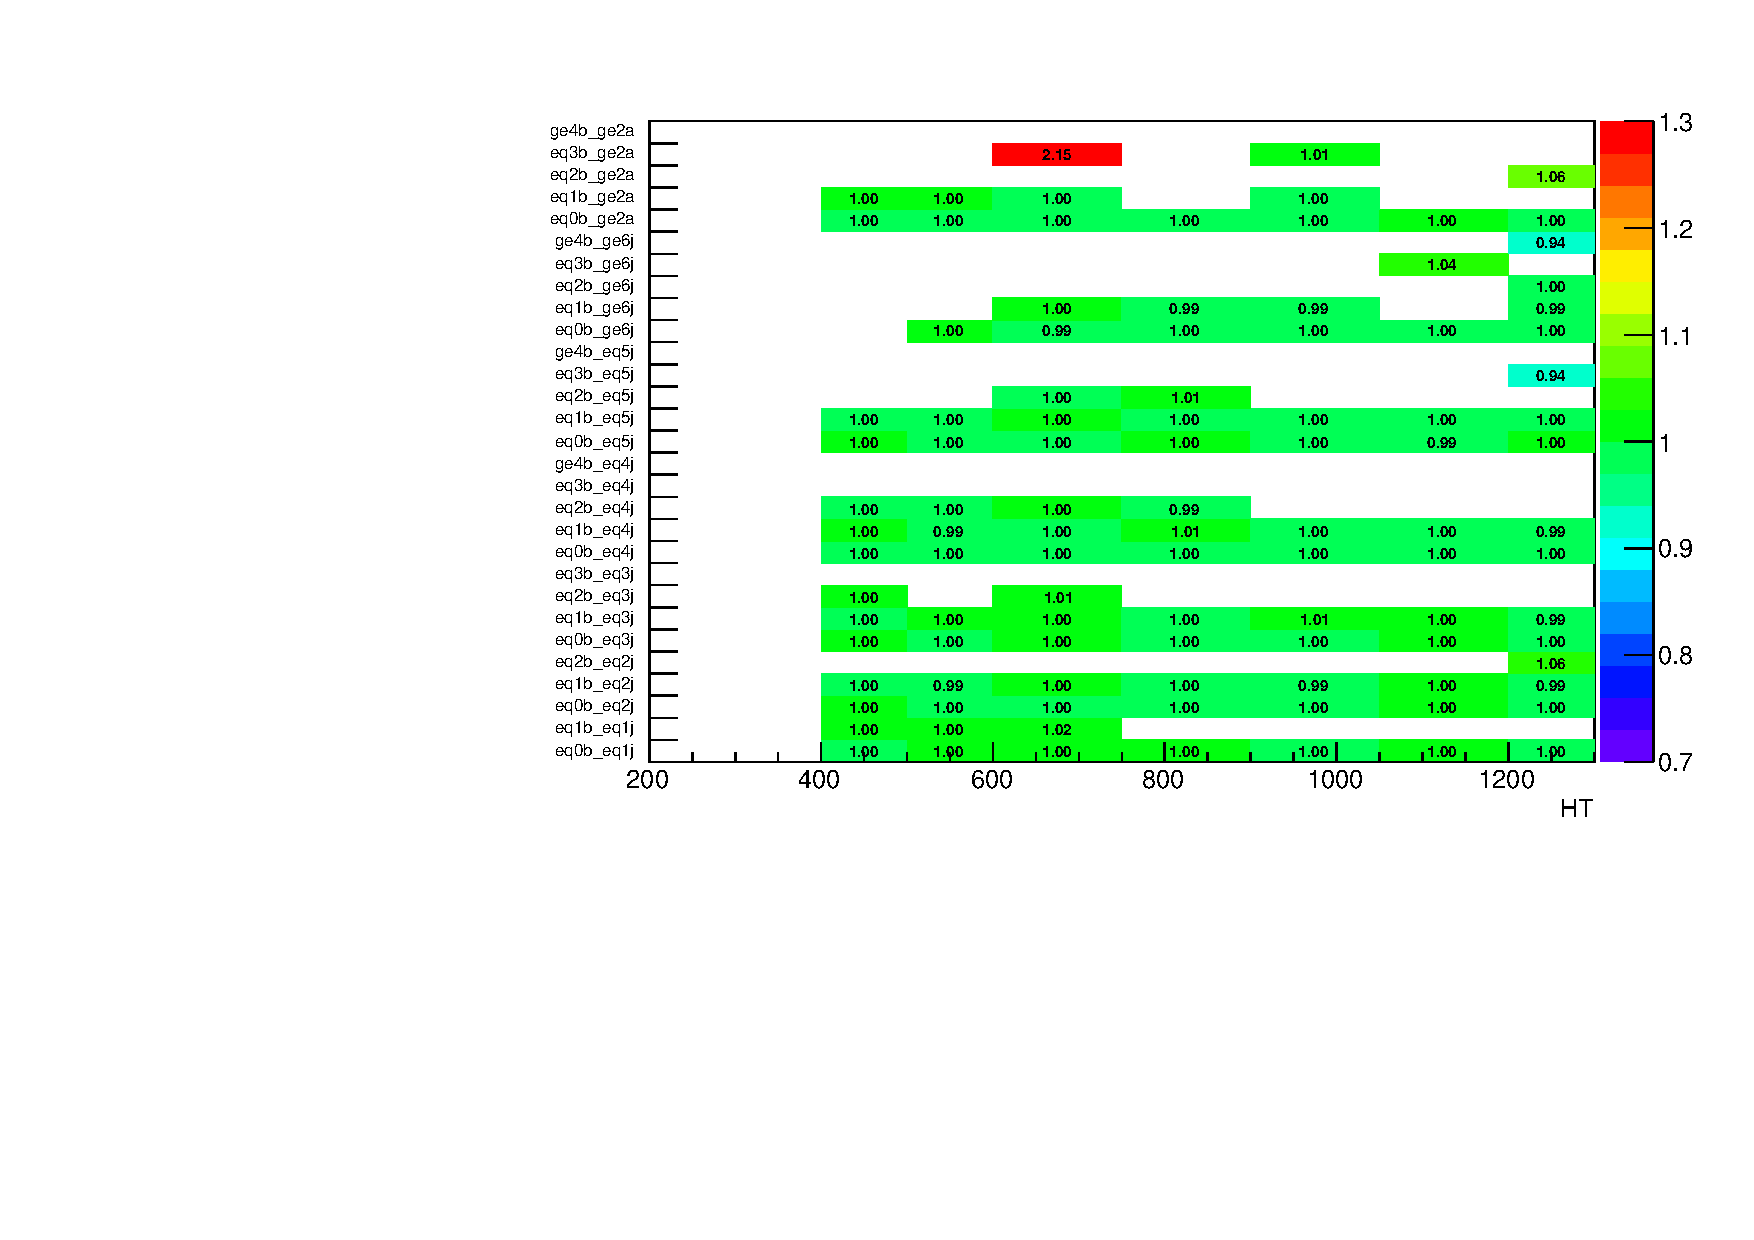
\includegraphics[width=0.5\textwidth]{figures/mcSystematics36p4fb/Zinv/gj/ratiotfh_ht_mht_allbsfWeight_Down.pdf}
  }\\

  \caption{\label{fig:tfSyst_bsf_gjToZinv} The relative change in the
  $\gj \rightarrow (\znunu)$ transfer
  factors when varying b-tag SF for heavy jets in MC within its uncertainties, as a function of \scalht and jet category. 
  Variations corresponding to $+1\sigma$ ($-1\sigma$) are shown in the left (right) figure. 
  }
\end{figure}

\begin{figure}[!h]
  \centering
  \subfigure[b-tag SF (heavy) up variation]{
    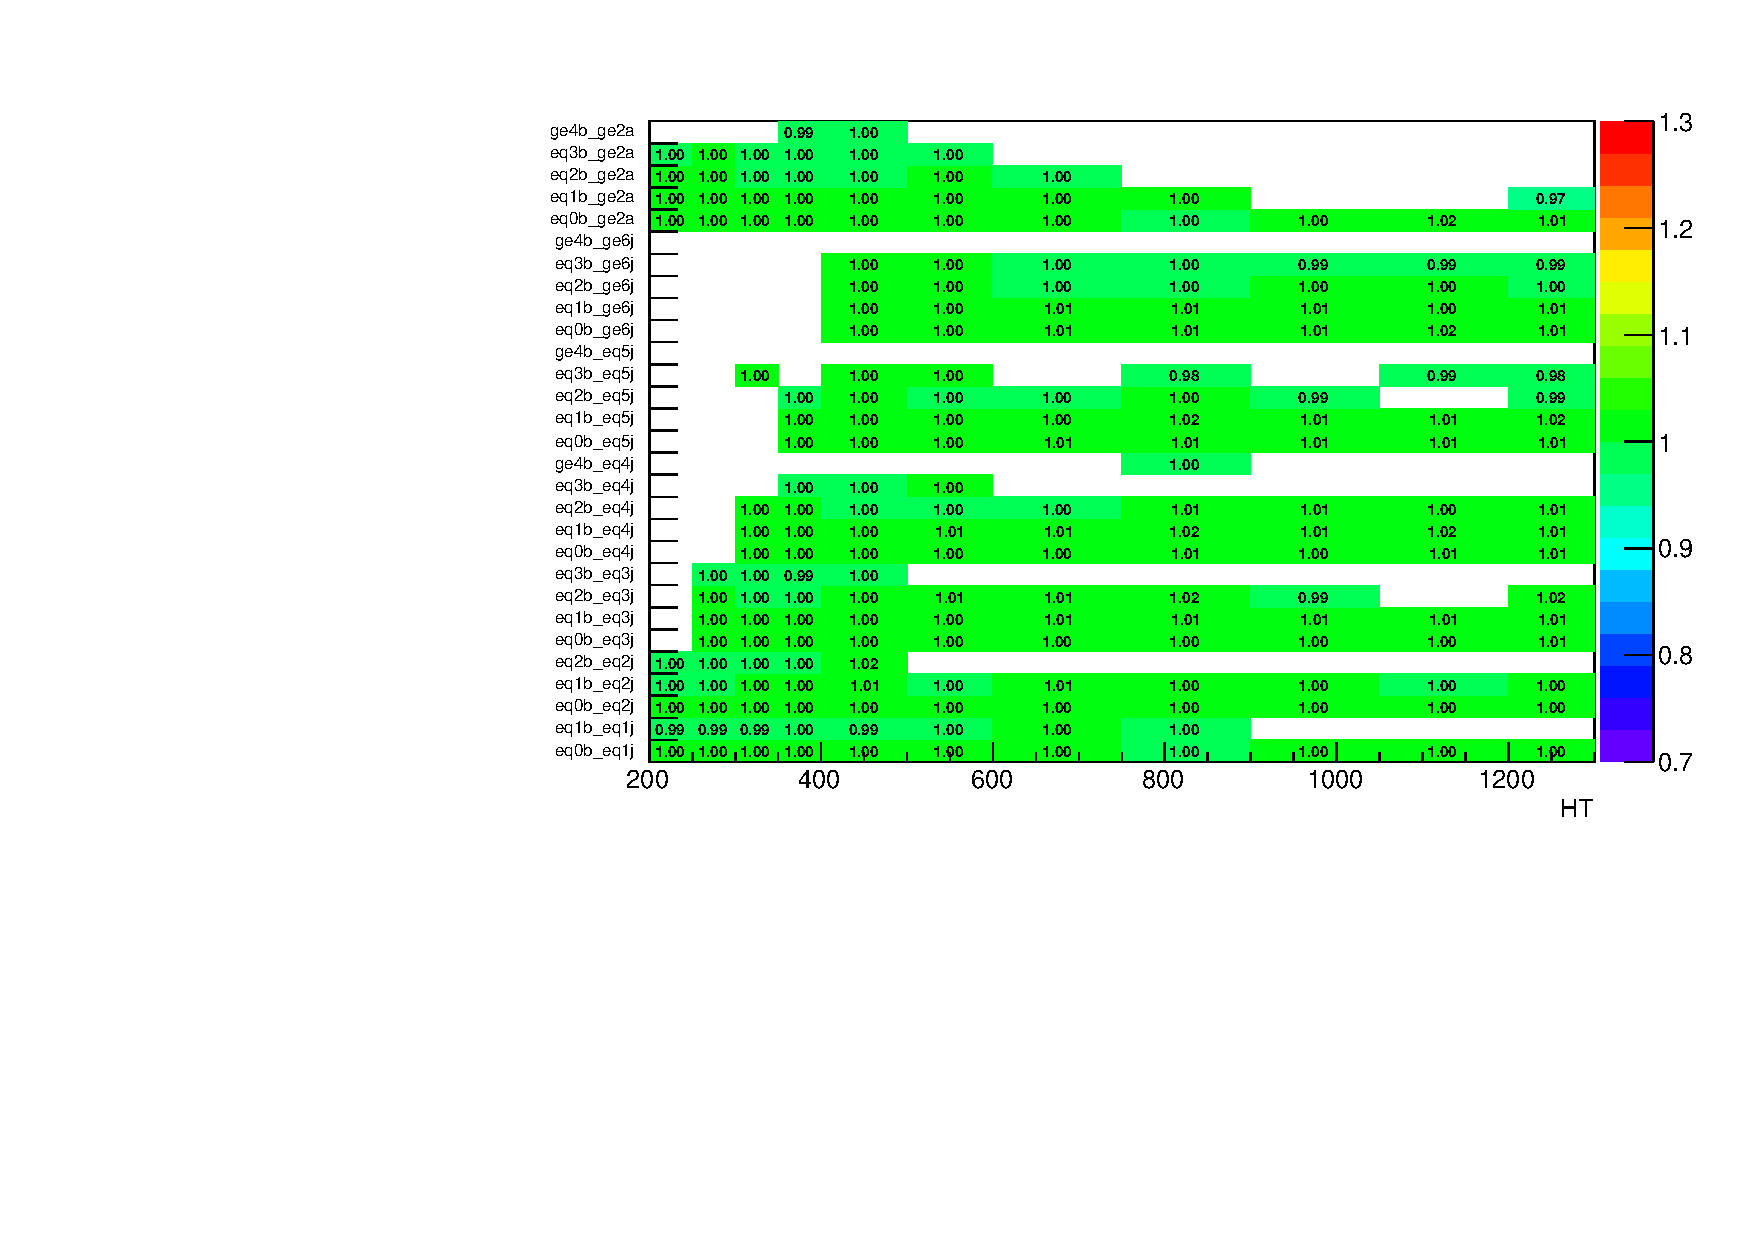
\includegraphics[width=0.5\textwidth]{figures/mcSystematics36p4fb/Ttw/mu/ratiotfh_ht_mht_allbsfWeight_Up.pdf}
  } ~~
  \subfigure[b-tag SF (heavy) down variation]{
    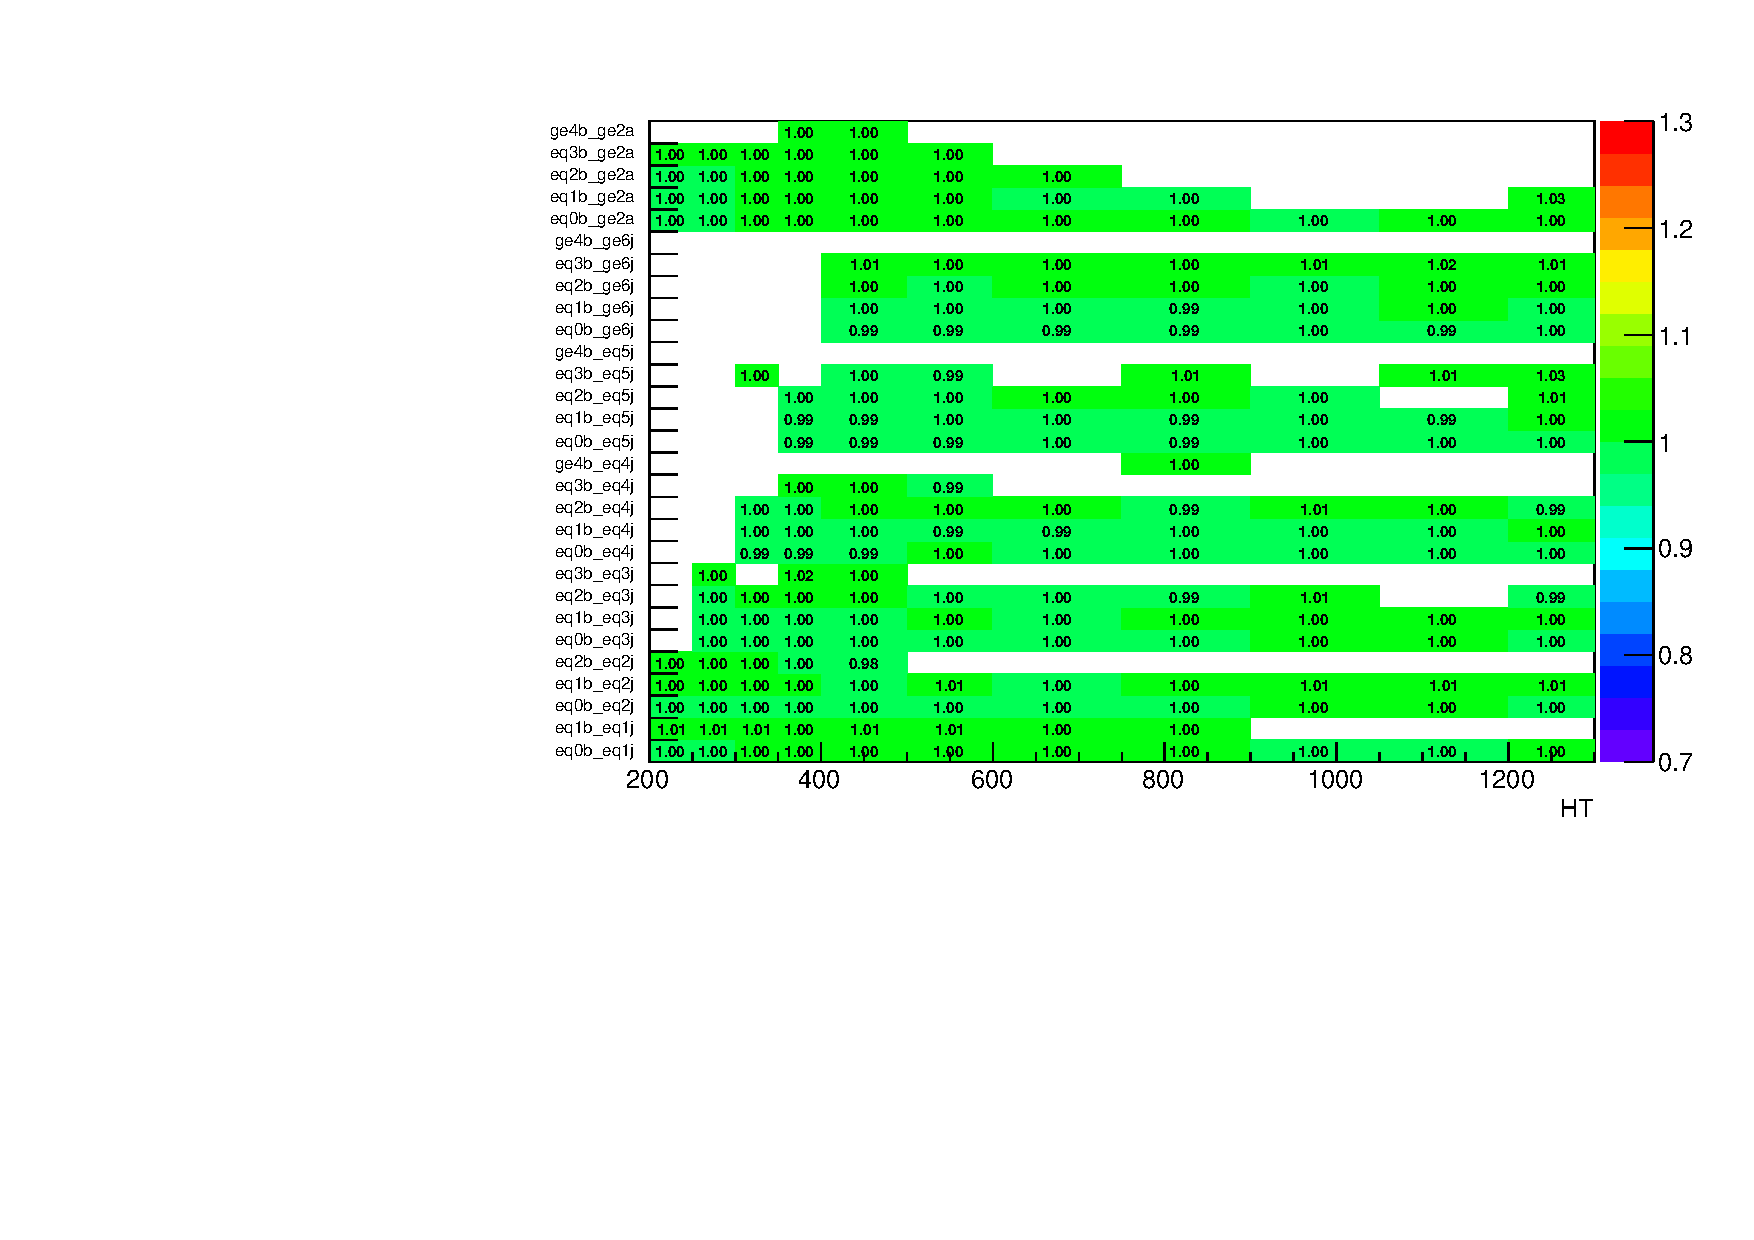
\includegraphics[width=0.5\textwidth]{figures/mcSystematics36p4fb/Ttw/mu/ratiotfh_ht_mht_allbsfWeight_Down.pdf}
  }\\

  \caption{\label{fig:tfSyst_bsf_muToTtw} The relative change in the $\mj \rightarrow \mathrm{tt+W}$ transfer
  factors when varying b-tag SF for heavy jets in MC within its uncertainties, as a function of \scalht and jet category. 
  Variations corresponding to $+1\sigma$ ($-1\sigma$) are shown in the left (right) figure. 
  }
\end{figure}

\begin{figure}[!h]
  \centering
  \subfigure[b-tag SF (light) up variation]{
    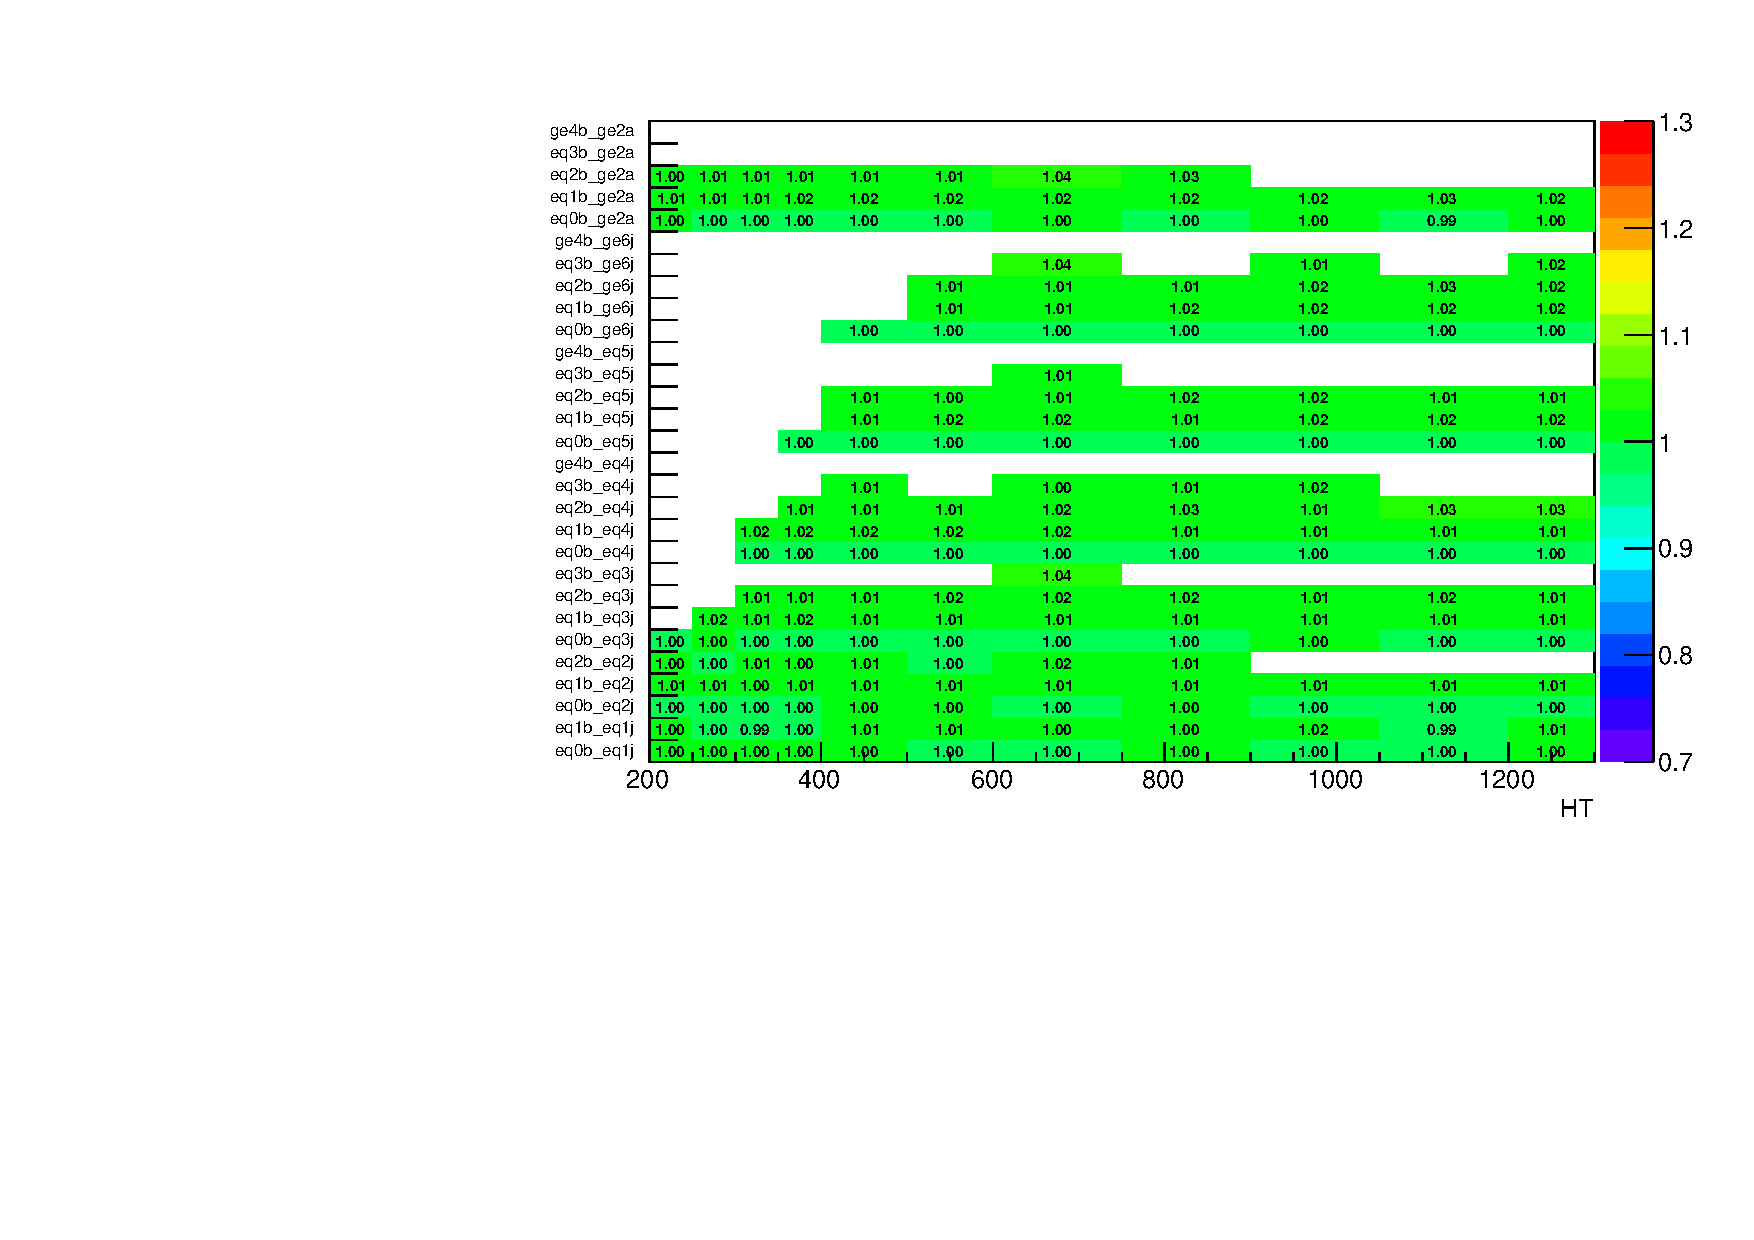
\includegraphics[width=0.5\textwidth]{figures/mcSystematics36p4fb/Zinv/mu/ratiotfh_ht_mht_allbsfLightWeight_Up.pdf}
  } ~~
  \subfigure[b-tag SF (light) down variation]{
    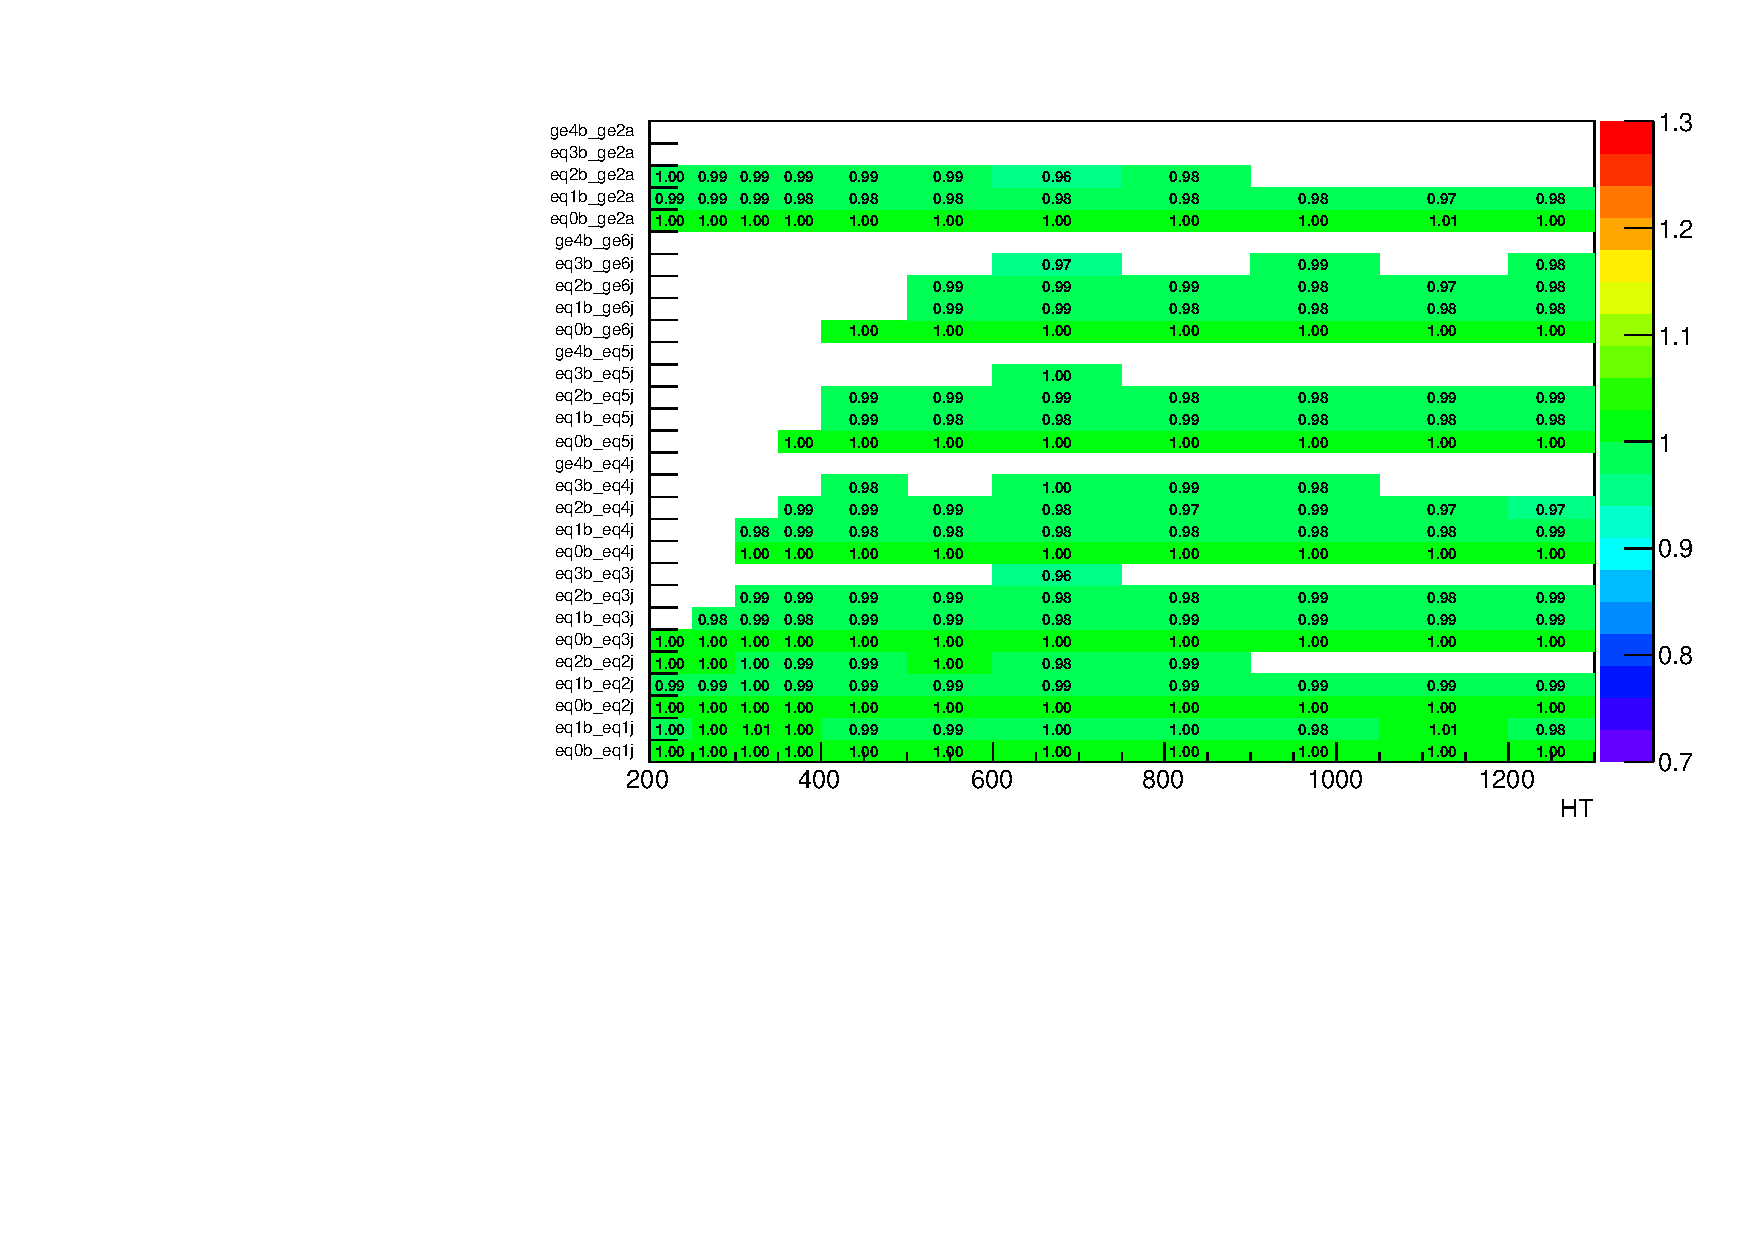
\includegraphics[width=0.5\textwidth]{figures/mcSystematics36p4fb/Zinv/mu/ratiotfh_ht_mht_allbsfLightWeight_Down.pdf}
  }\\

  \caption{\label{fig:tfSyst_bsfl_muToZinv} The relative change in the
  $\mj \rightarrow (\znunu)$ transfer
  factors when varying b-tag SF for light jets in MC within its uncertainties, as a function of \scalht and jet category. 
  Variations corresponding to $+1\sigma$ ($-1\sigma$) are shown in the left (right) figure. 
  }
\end{figure}

\begin{figure}[!h]
  \centering
  \subfigure[b-tag SF (light) up variation]{
    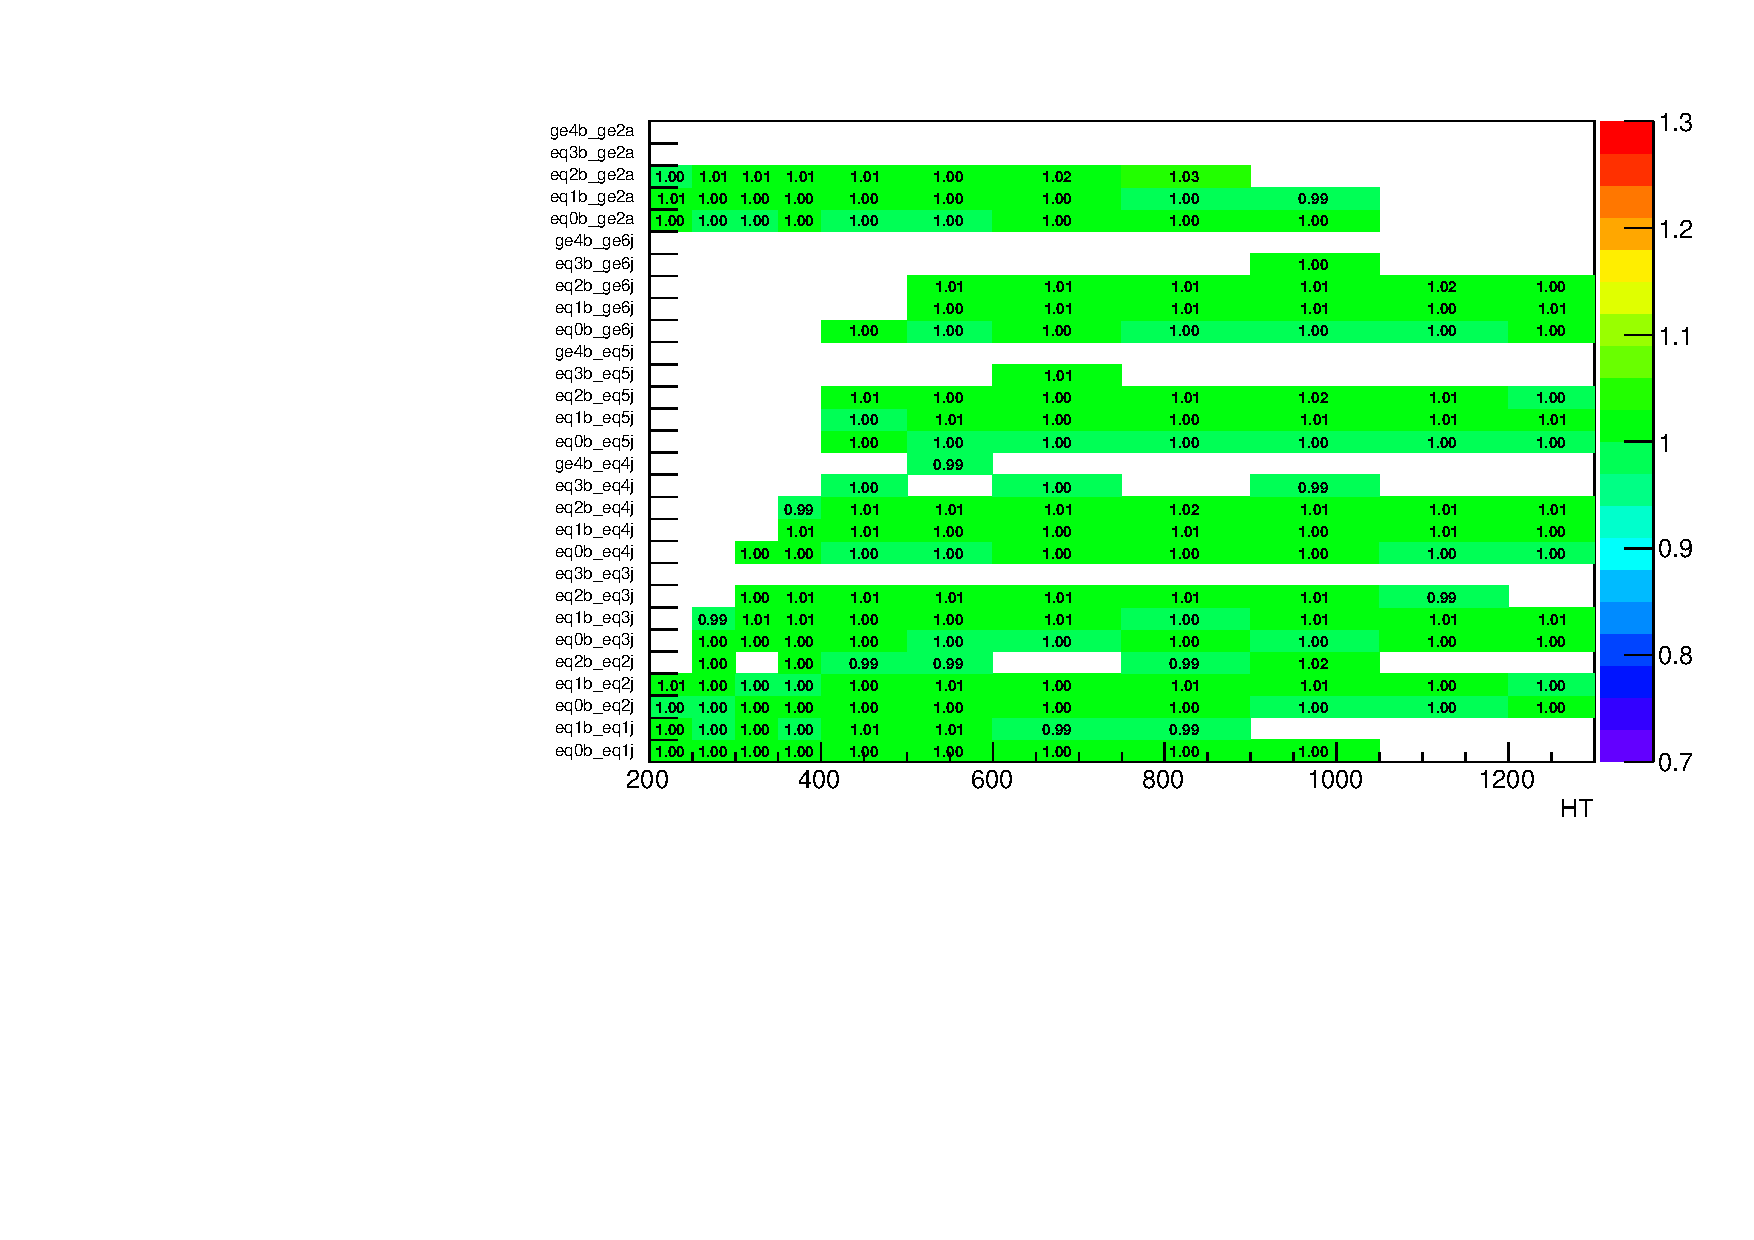
\includegraphics[width=0.5\textwidth]{figures/mcSystematics36p4fb/Zinv/mumu/ratiotfh_ht_mht_allbsfLightWeight_Up.pdf}
  } ~~
  \subfigure[b-tag SF (light) down variation]{
    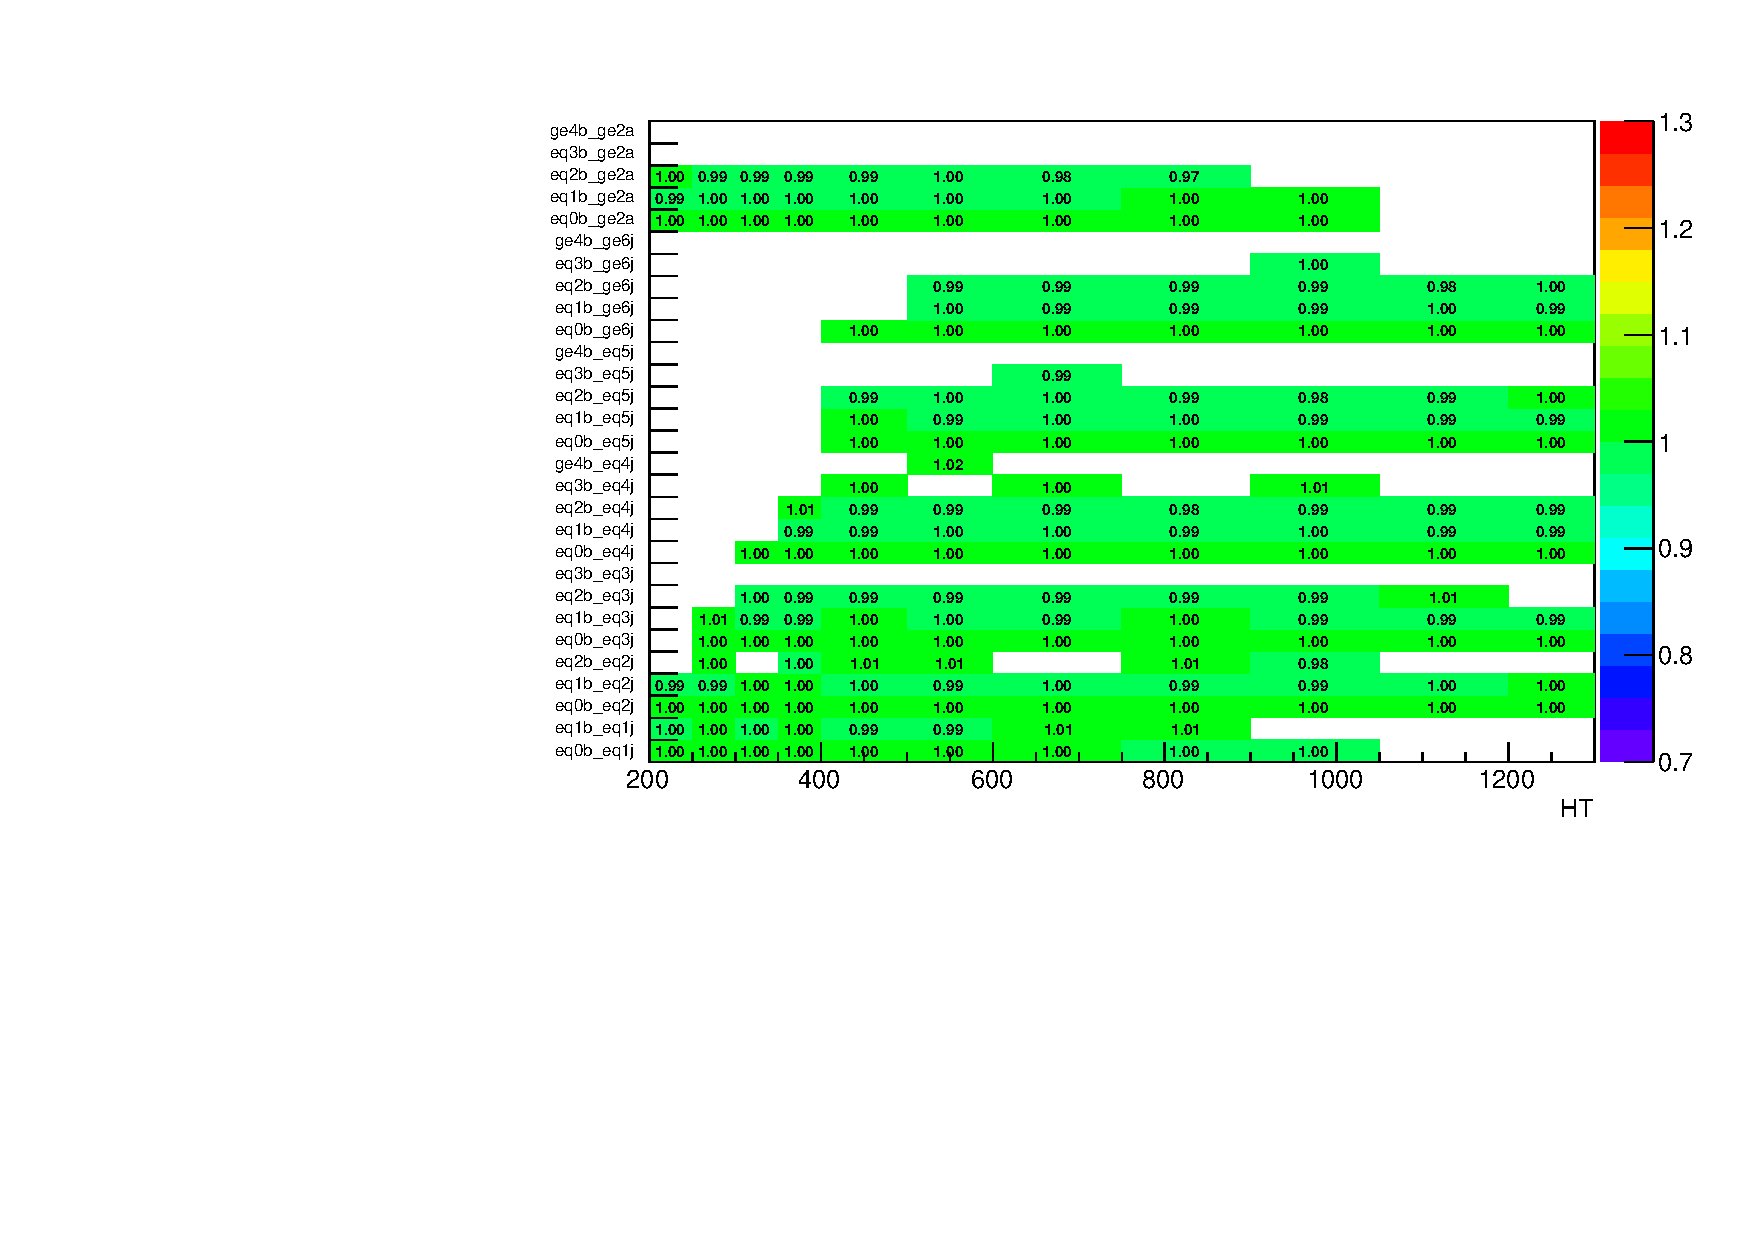
\includegraphics[width=0.5\textwidth]{figures/mcSystematics36p4fb/Zinv/mumu/ratiotfh_ht_mht_allbsfLightWeight_Down.pdf}
  }\\

  \caption{\label{fig:tfSyst_bsfl_mumuToZinv} The relative change in
  the $\mmj \rightarrow (\znunu)$ transfer
  factors when varying b-tag SF for light jets in MC within its uncertainties, as a function of \scalht and jet category. 
  Variations corresponding to $+1\sigma$ ($-1\sigma$) are shown in the left (right) figure. 
  }
\end{figure}

\begin{figure}[!h]
  \centering
  \subfigure[b-tag SF (light) up variation]{
    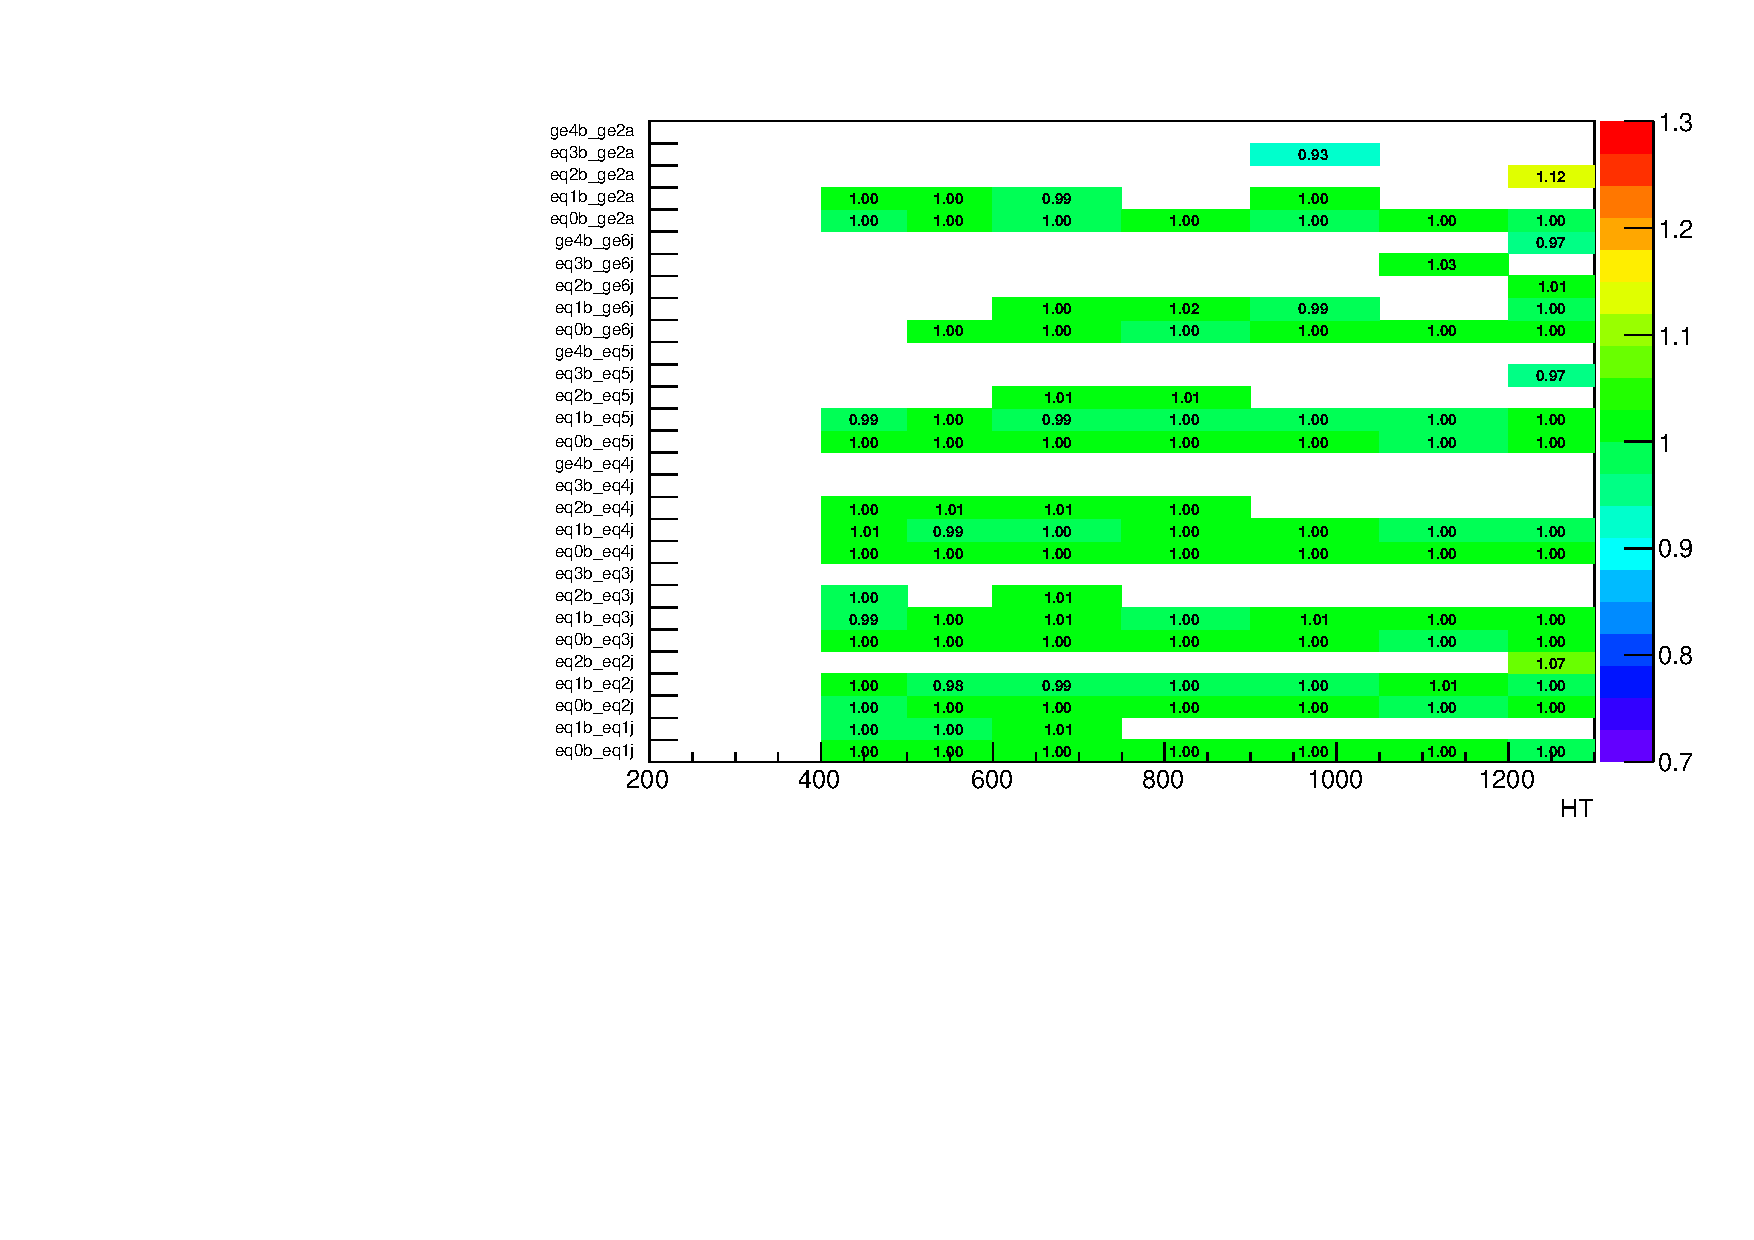
\includegraphics[width=0.5\textwidth]{figures/mcSystematics36p4fb/Zinv/gj/ratiotfh_ht_mht_allbsfLightWeight_Up.pdf}
  } ~~
  \subfigure[b-tag SF (light) down variation]{
    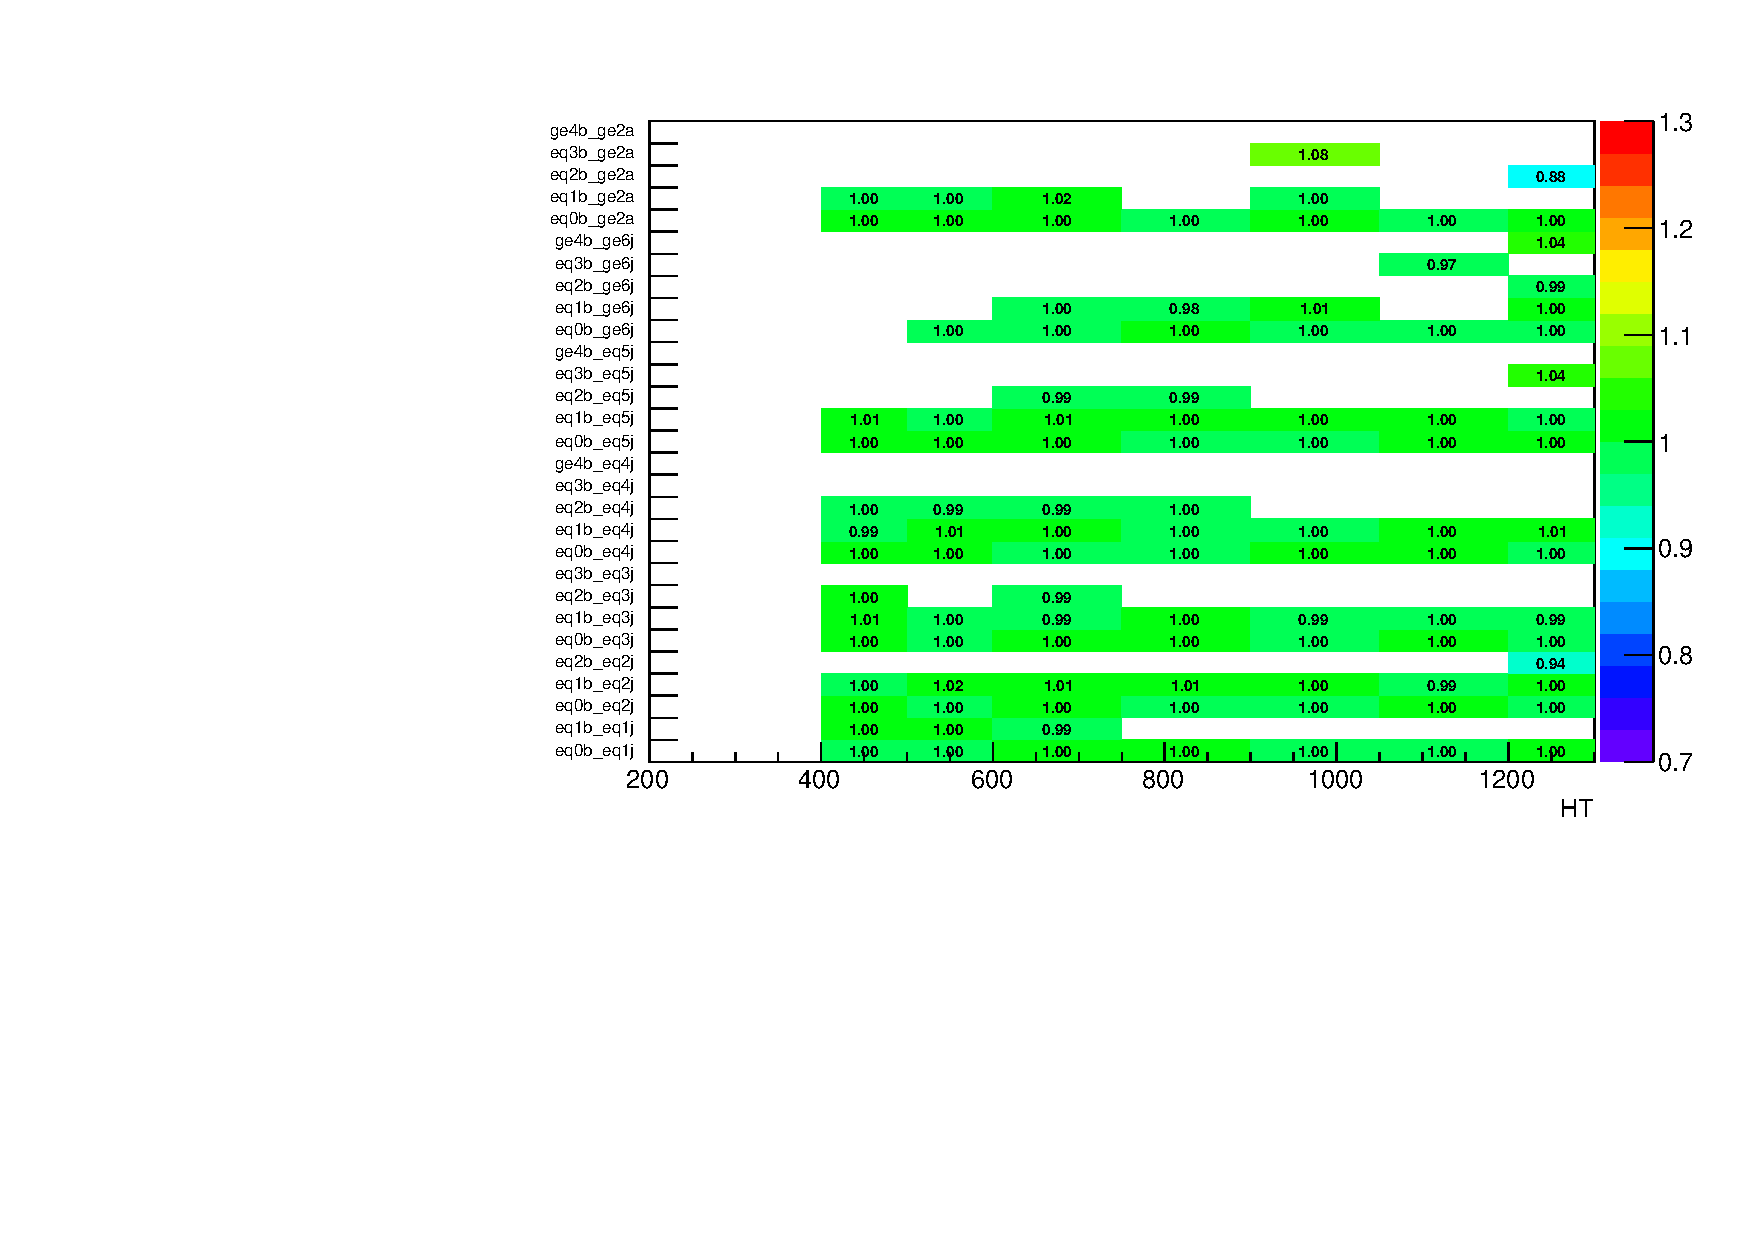
\includegraphics[width=0.5\textwidth]{figures/mcSystematics36p4fb/Zinv/gj/ratiotfh_ht_mht_allbsfLightWeight_Down.pdf}
  }\\

  \caption{\label{fig:tfSyst_bsfl_gjToZinv} The relative change in the
  $\gj \rightarrow (\znunu)$ transfer
  factors when varying b-tag SF for light jets in MC within its uncertainties, as a function of \scalht and jet category. 
  Variations corresponding to $+1\sigma$ ($-1\sigma$) are shown in the left (right) figure. 
  }
\end{figure}

\begin{figure}[!h]
  \centering
  \subfigure[b-tag SF (light) up variation]{
    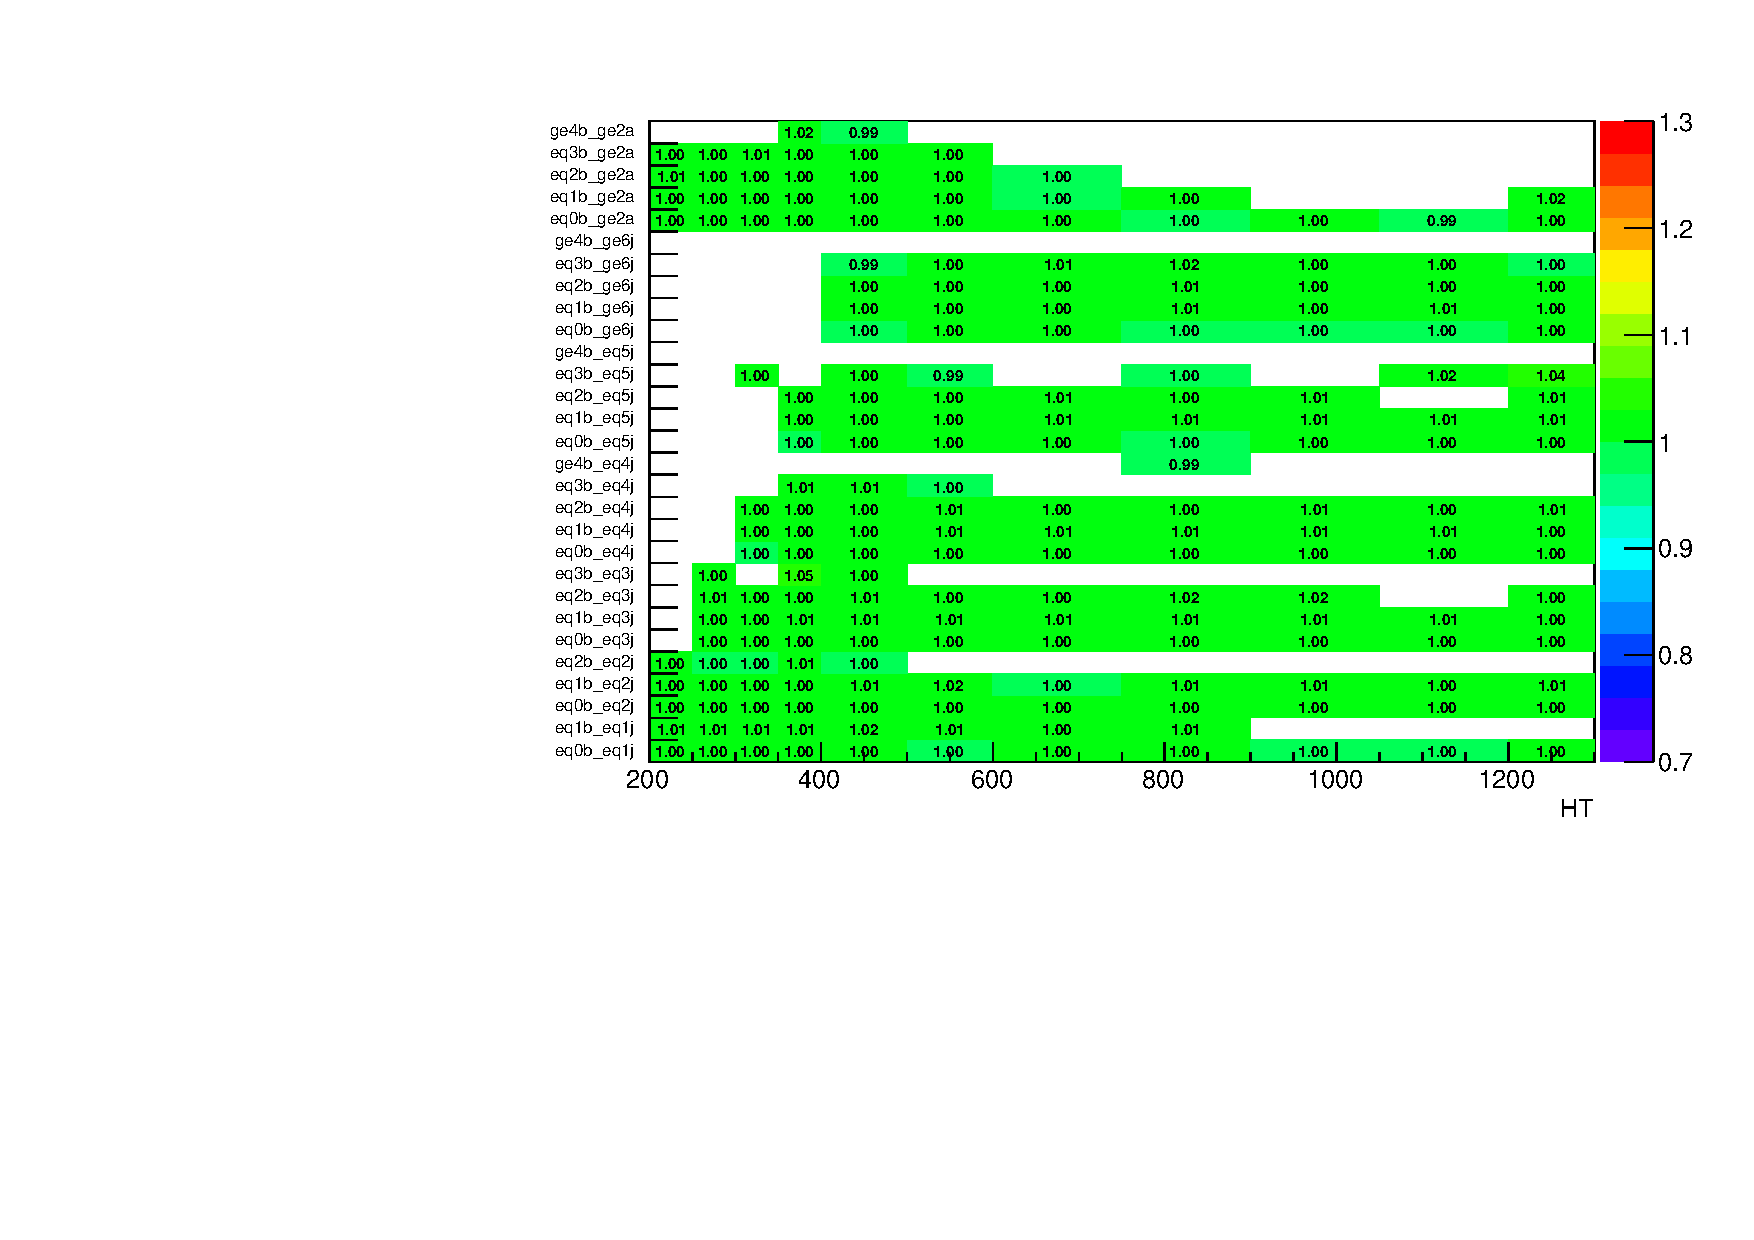
\includegraphics[width=0.5\textwidth]{figures/mcSystematics36p4fb/Ttw/mu/ratiotfh_ht_mht_allbsfLightWeight_Up.pdf}
  } ~~
  \subfigure[b-tag SF (light) down variation]{
    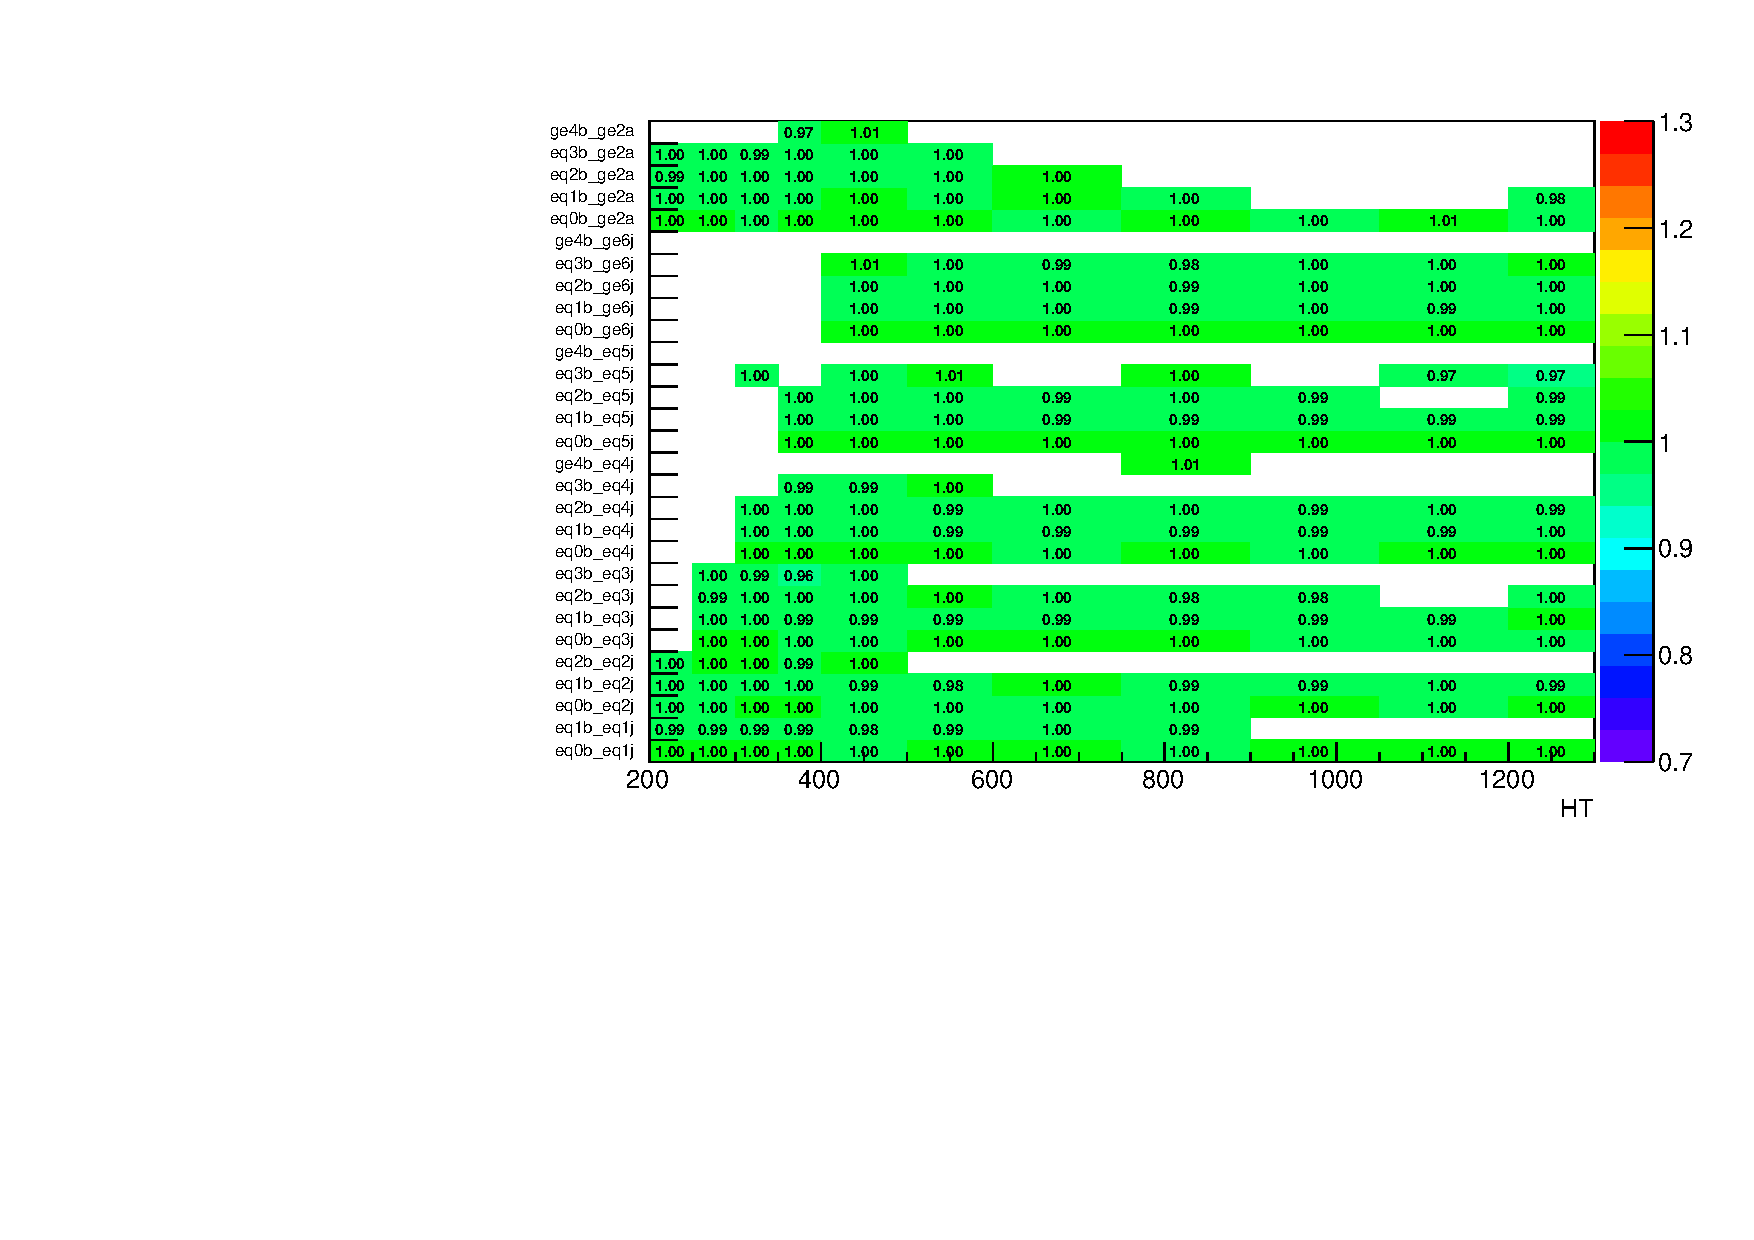
\includegraphics[width=0.5\textwidth]{figures/mcSystematics36p4fb/Ttw/mu/ratiotfh_ht_mht_allbsfLightWeight_Down.pdf}
  }\\

  \caption{\label{fig:tfSyst_bsfl_muToTtw} The relative change in the $\mj \rightarrow \mathrm{tt+W}$ transfer
  factors when varying b-tag SF for light jets in MC within its uncertainties, as a function of \scalht and jet category. 
  Variations corresponding to $+1\sigma$ ($-1\sigma$) are shown in the left (right) figure. 
  }
\end{figure}

\clearpage
\subsection{Lepton and photon trigger/identification/isolation efficiency}

\begin{figure}[!h]
  \centering
  \subfigure[muon scale factor up variation]{
    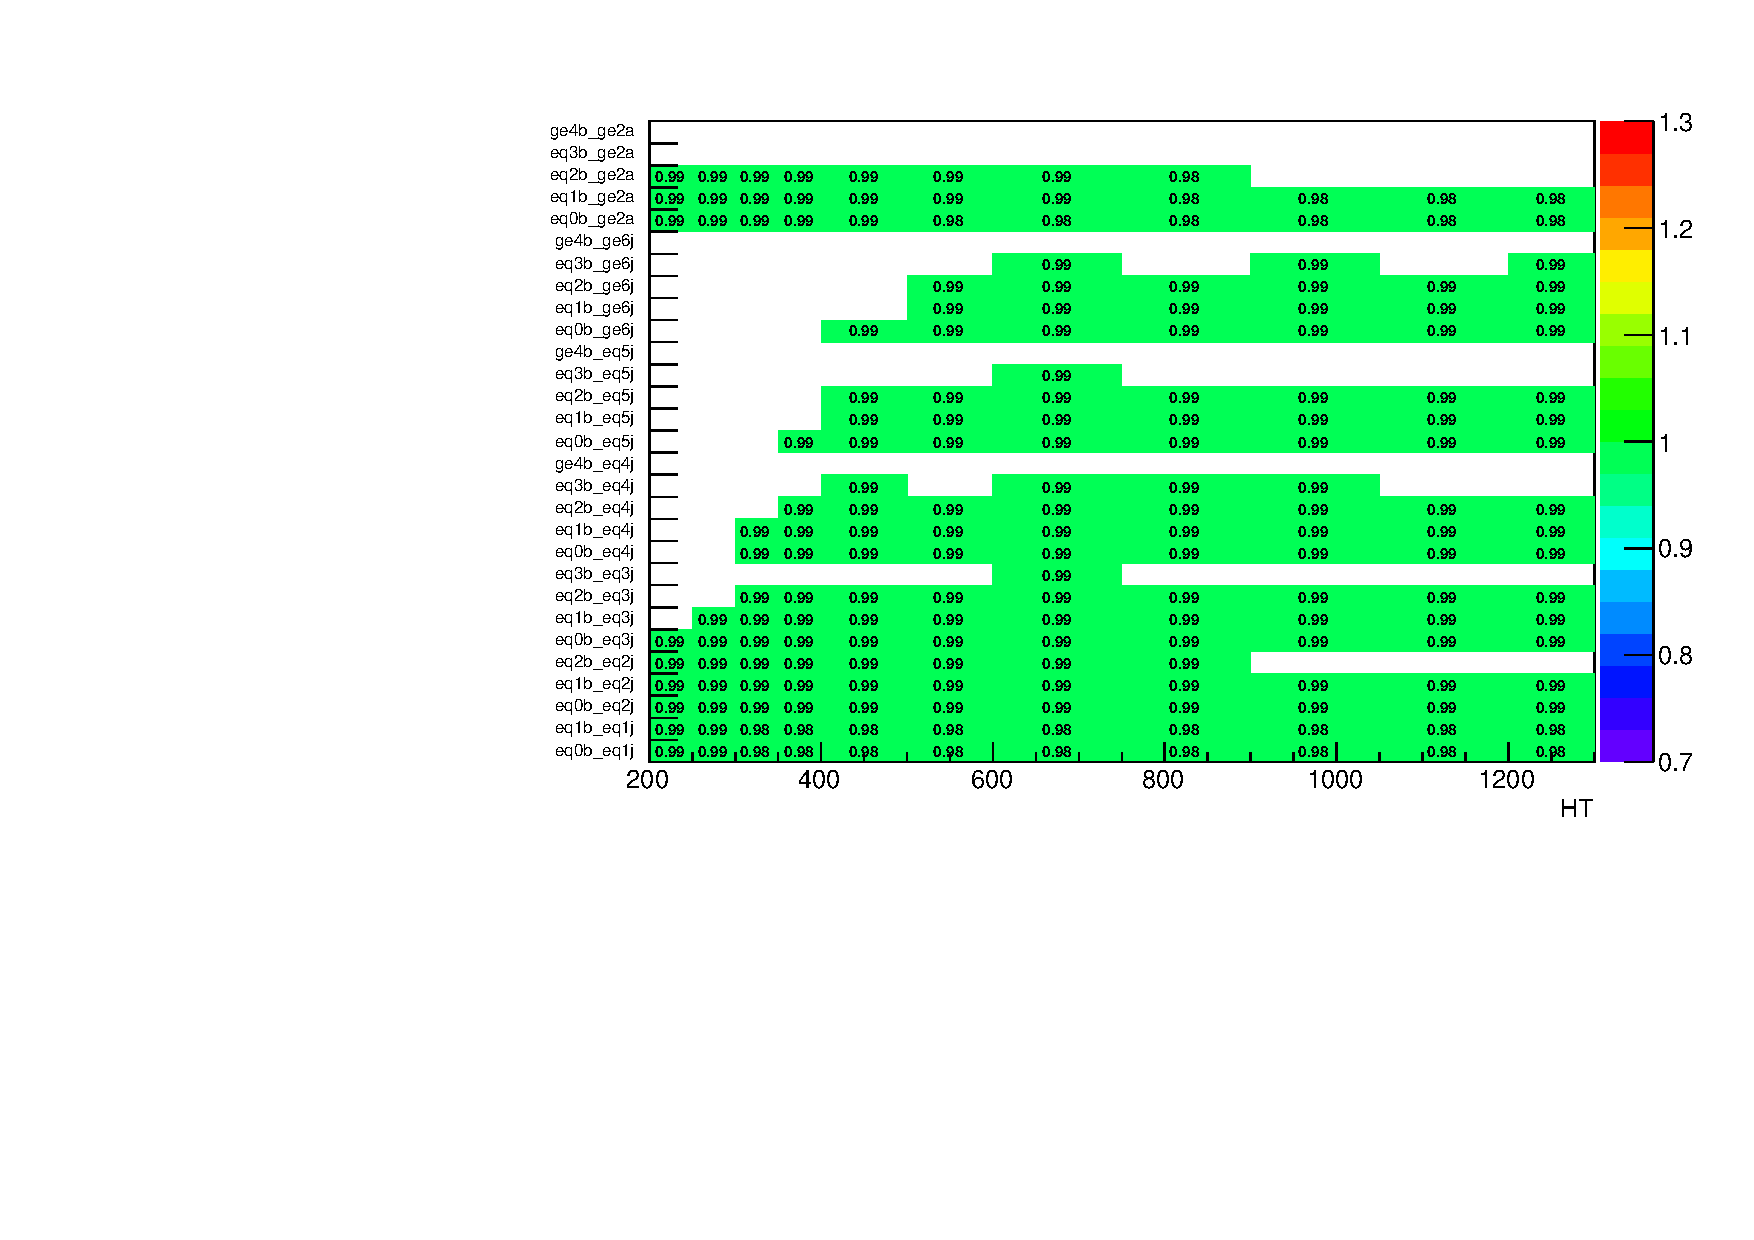
\includegraphics[width=0.5\textwidth]{figures/mcSystematics36p4fb/Zinv/mu/ratiotfh_ht_mht_allmuonSfWeight_Up.pdf}
  } ~~
  \subfigure[muon scale factor down variation]{
    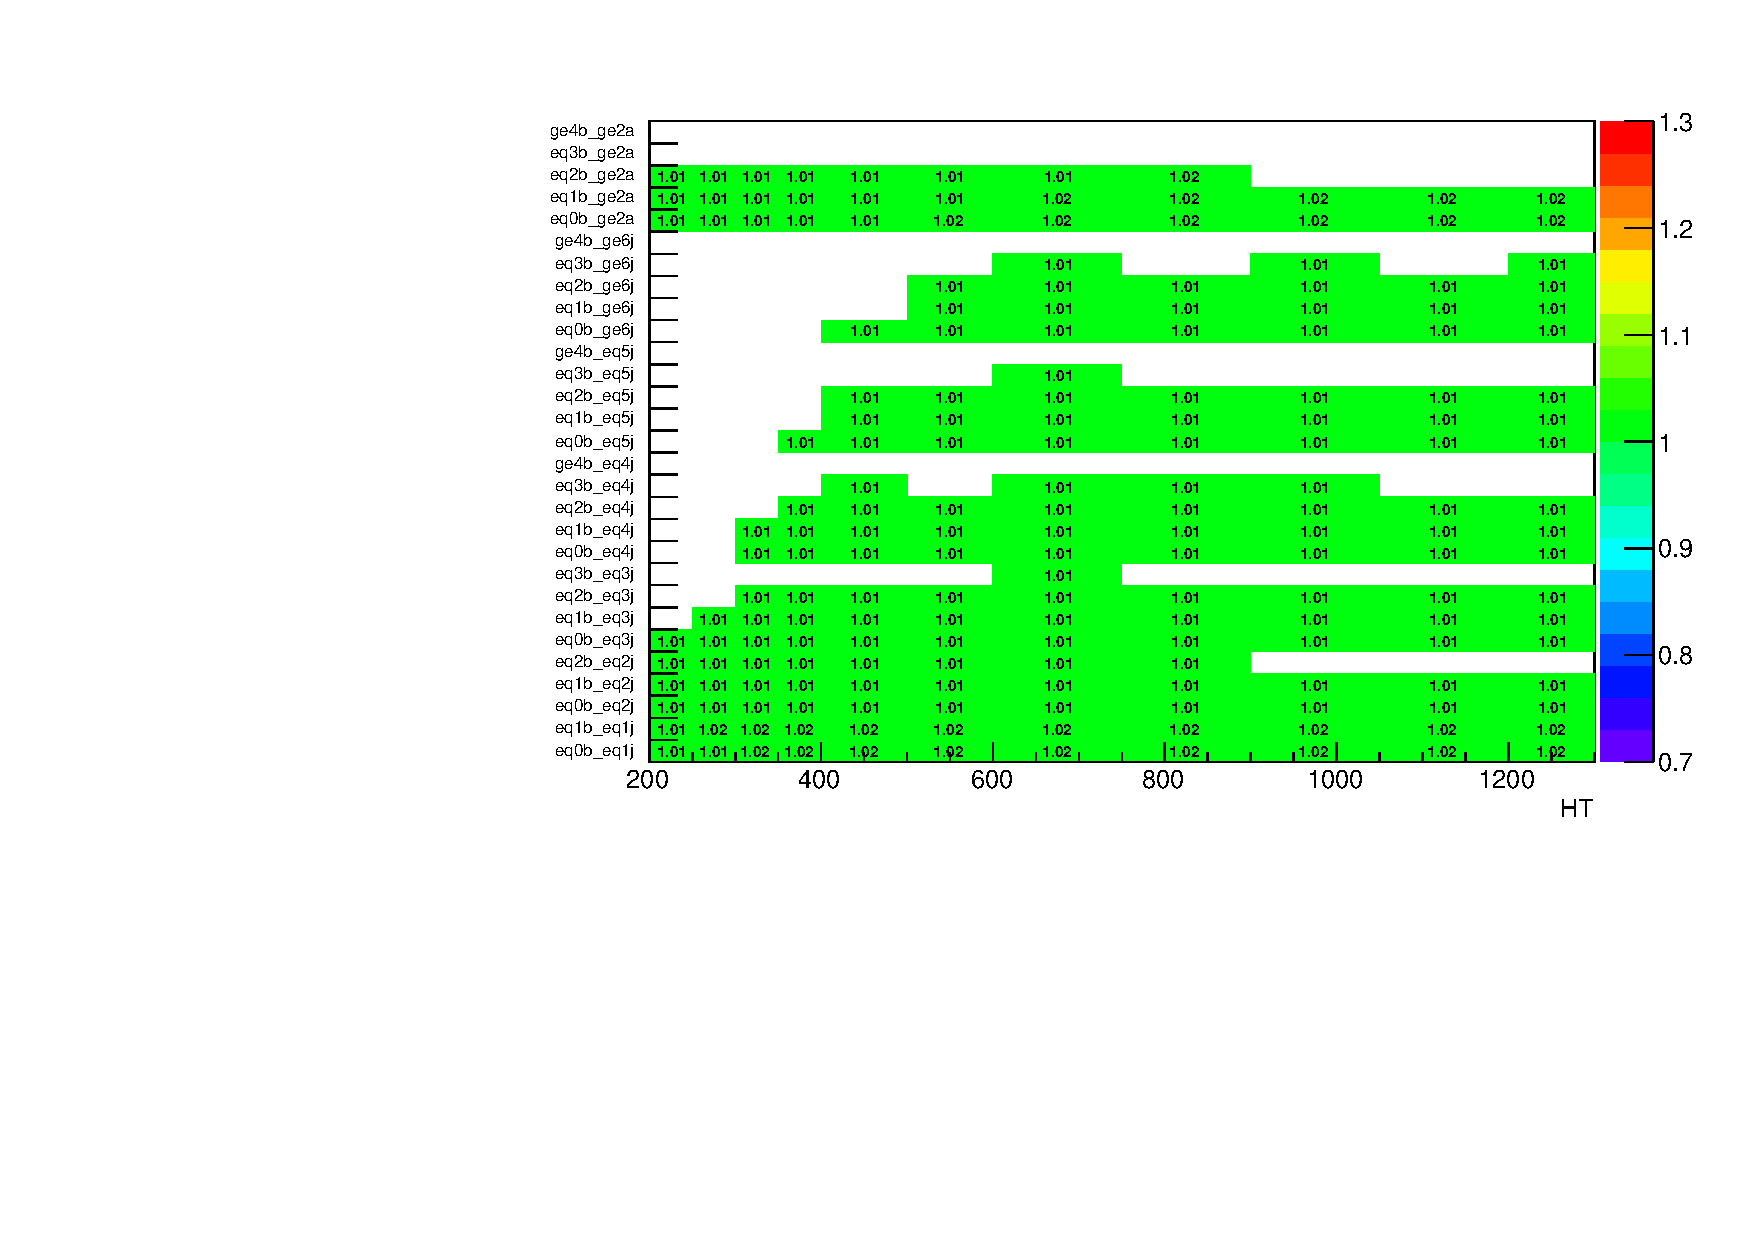
\includegraphics[width=0.5\textwidth]{figures/mcSystematics36p4fb/Zinv/mu/ratiotfh_ht_mht_allmuonSfWeight_Down.pdf}
  }\\

  \caption{\label{fig:tfSyst_muon scale factor_muToZinv} The relative change in
  the $\mj \rightarrow (\znunu)$ transfer
  factors when varying muon scale factor in MC within its uncertainties, as a function of \scalht and jet category. 
  Variations corresponding to $+1\sigma$ ($-1\sigma$) are shown in the left (right) figure. 
  }
\end{figure}

\begin{figure}[!h]
  \centering
  \subfigure[muon scale factor up variation]{
    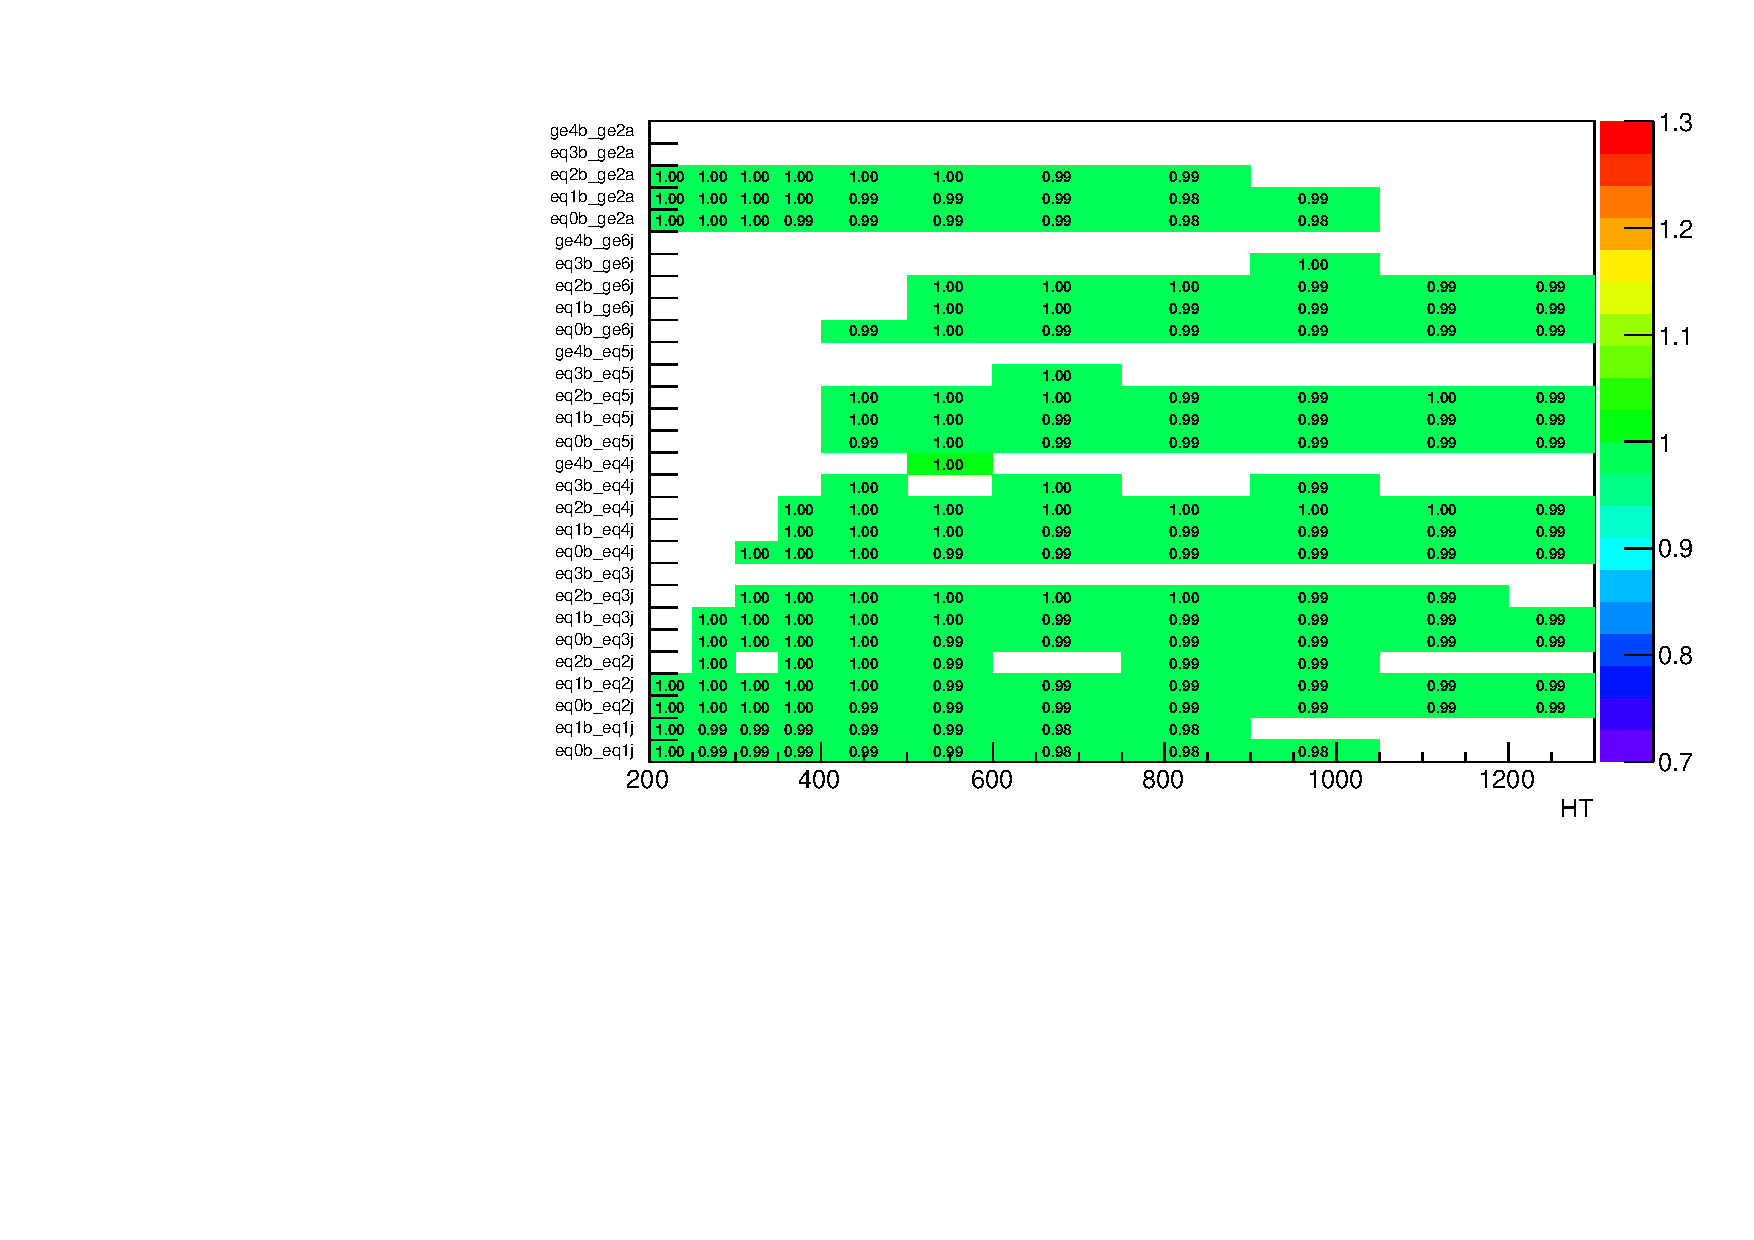
\includegraphics[width=0.5\textwidth]{figures/mcSystematics36p4fb/Zinv/mumu/ratiotfh_ht_mht_allmuonSfWeight_Up.pdf}
  } ~~
  \subfigure[muon scale factor down variation]{
    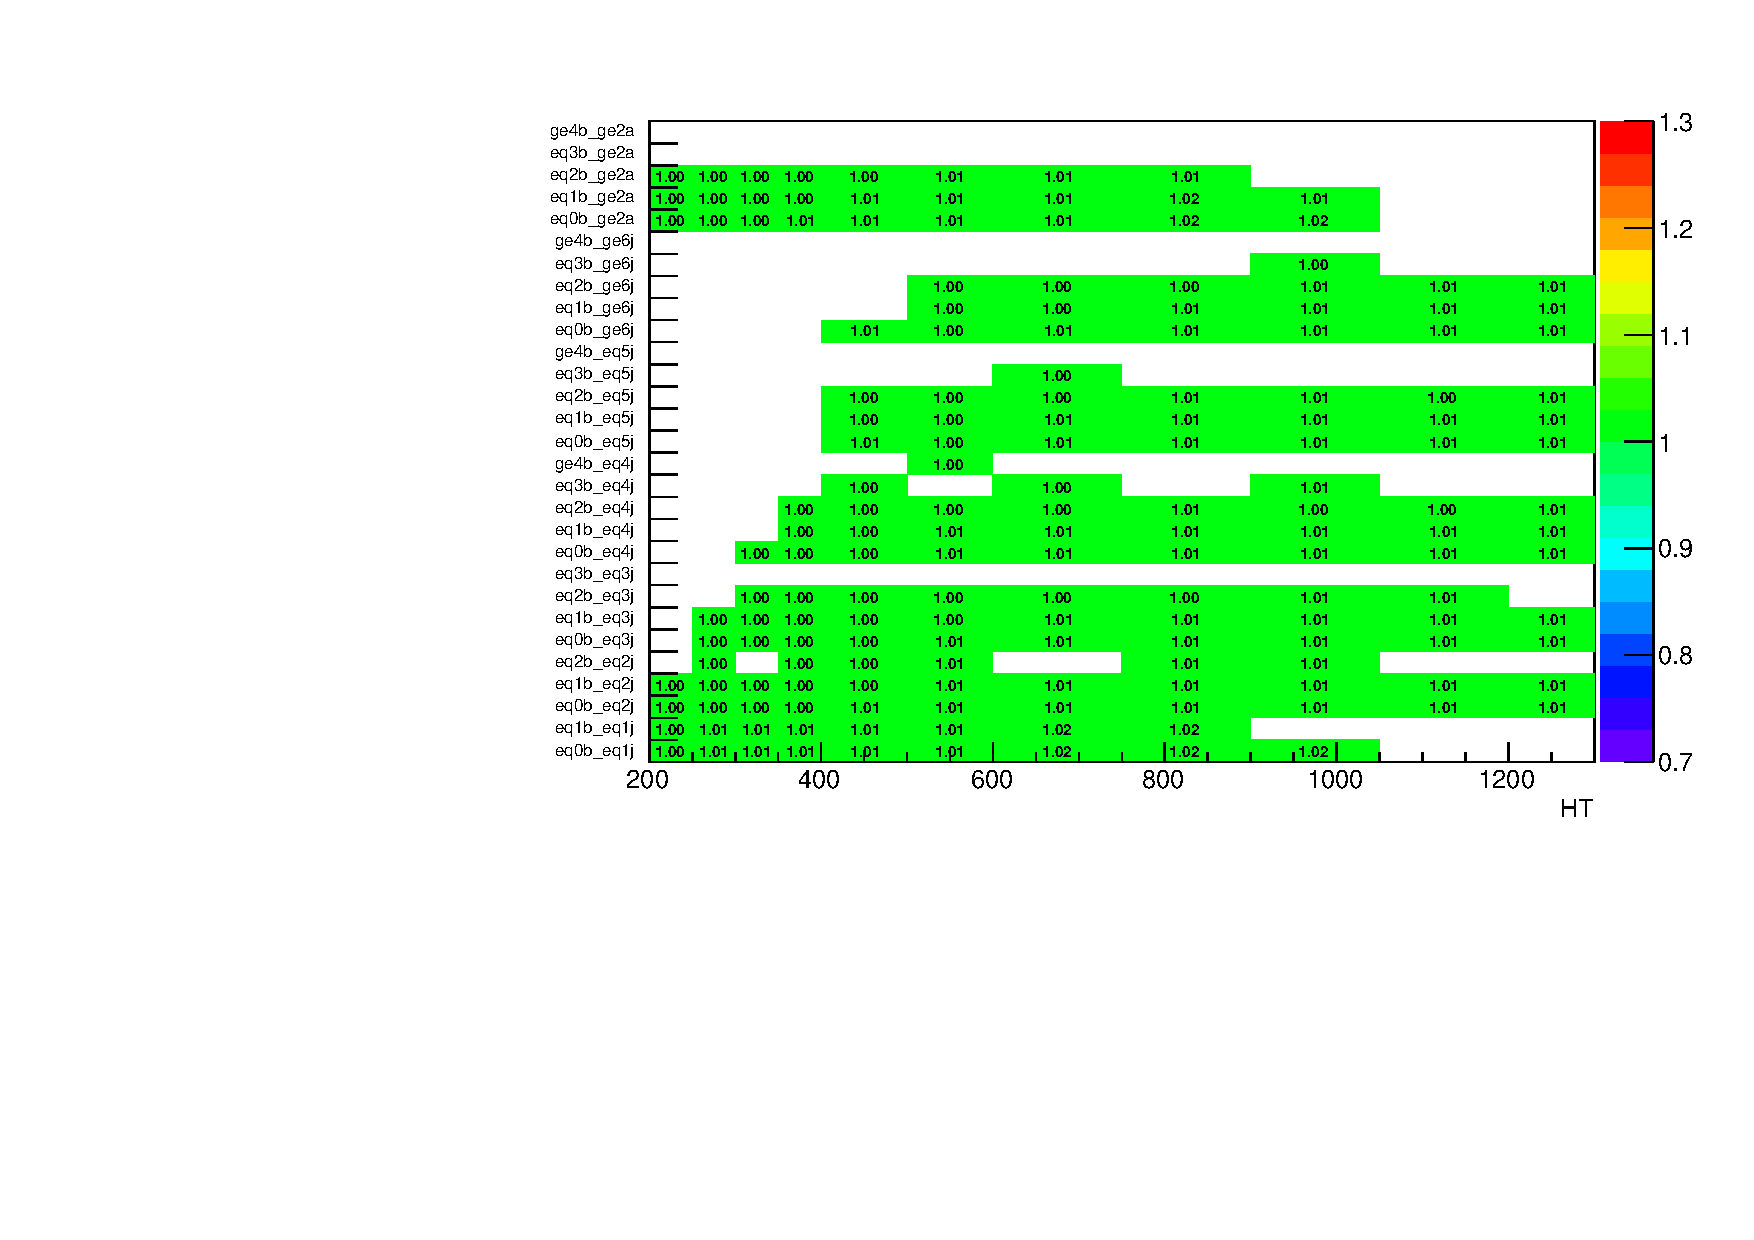
\includegraphics[width=0.5\textwidth]{figures/mcSystematics36p4fb/Zinv/mumu/ratiotfh_ht_mht_allmuonSfWeight_Down.pdf}
  }\\

  \caption{\label{fig:tfSyst_muon scale factor_mumuToZinv} The relative change in
  the $\mmj \rightarrow (\znunu)$ transfer
  factors when varying muon scale factor in MC within its uncertainties, as a function of \scalht and jet category. 
  Variations corresponding to $+1\sigma$ ($-1\sigma$) are shown in the left (right) figure. 
  }
\end{figure}

\begin{figure}[!h]
  \centering
  \subfigure[muon scale factor up variation]{
    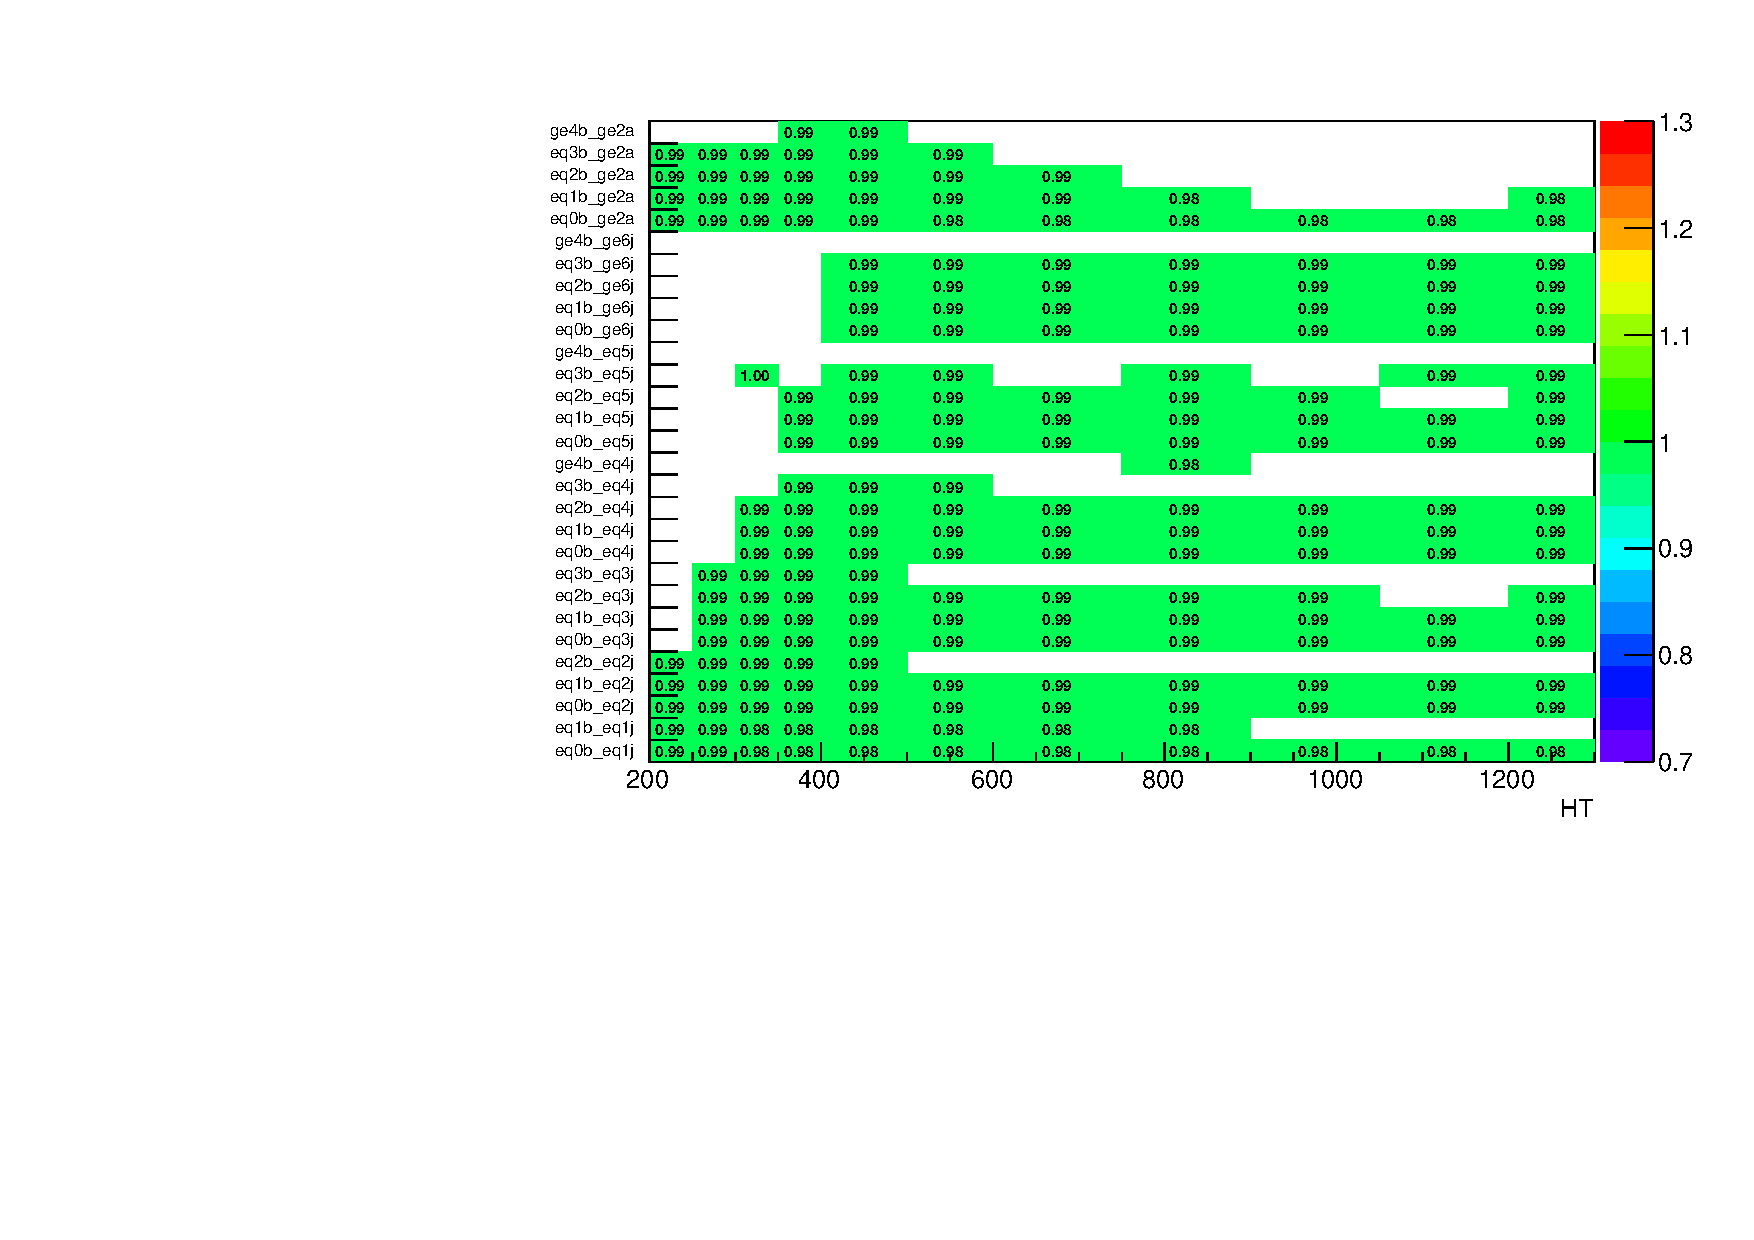
\includegraphics[width=0.5\textwidth]{figures/mcSystematics36p4fb/Ttw/mu/ratiotfh_ht_mht_allmuonSfWeight_Up.pdf}
  } ~~
  \subfigure[muon scale factor down variation]{
    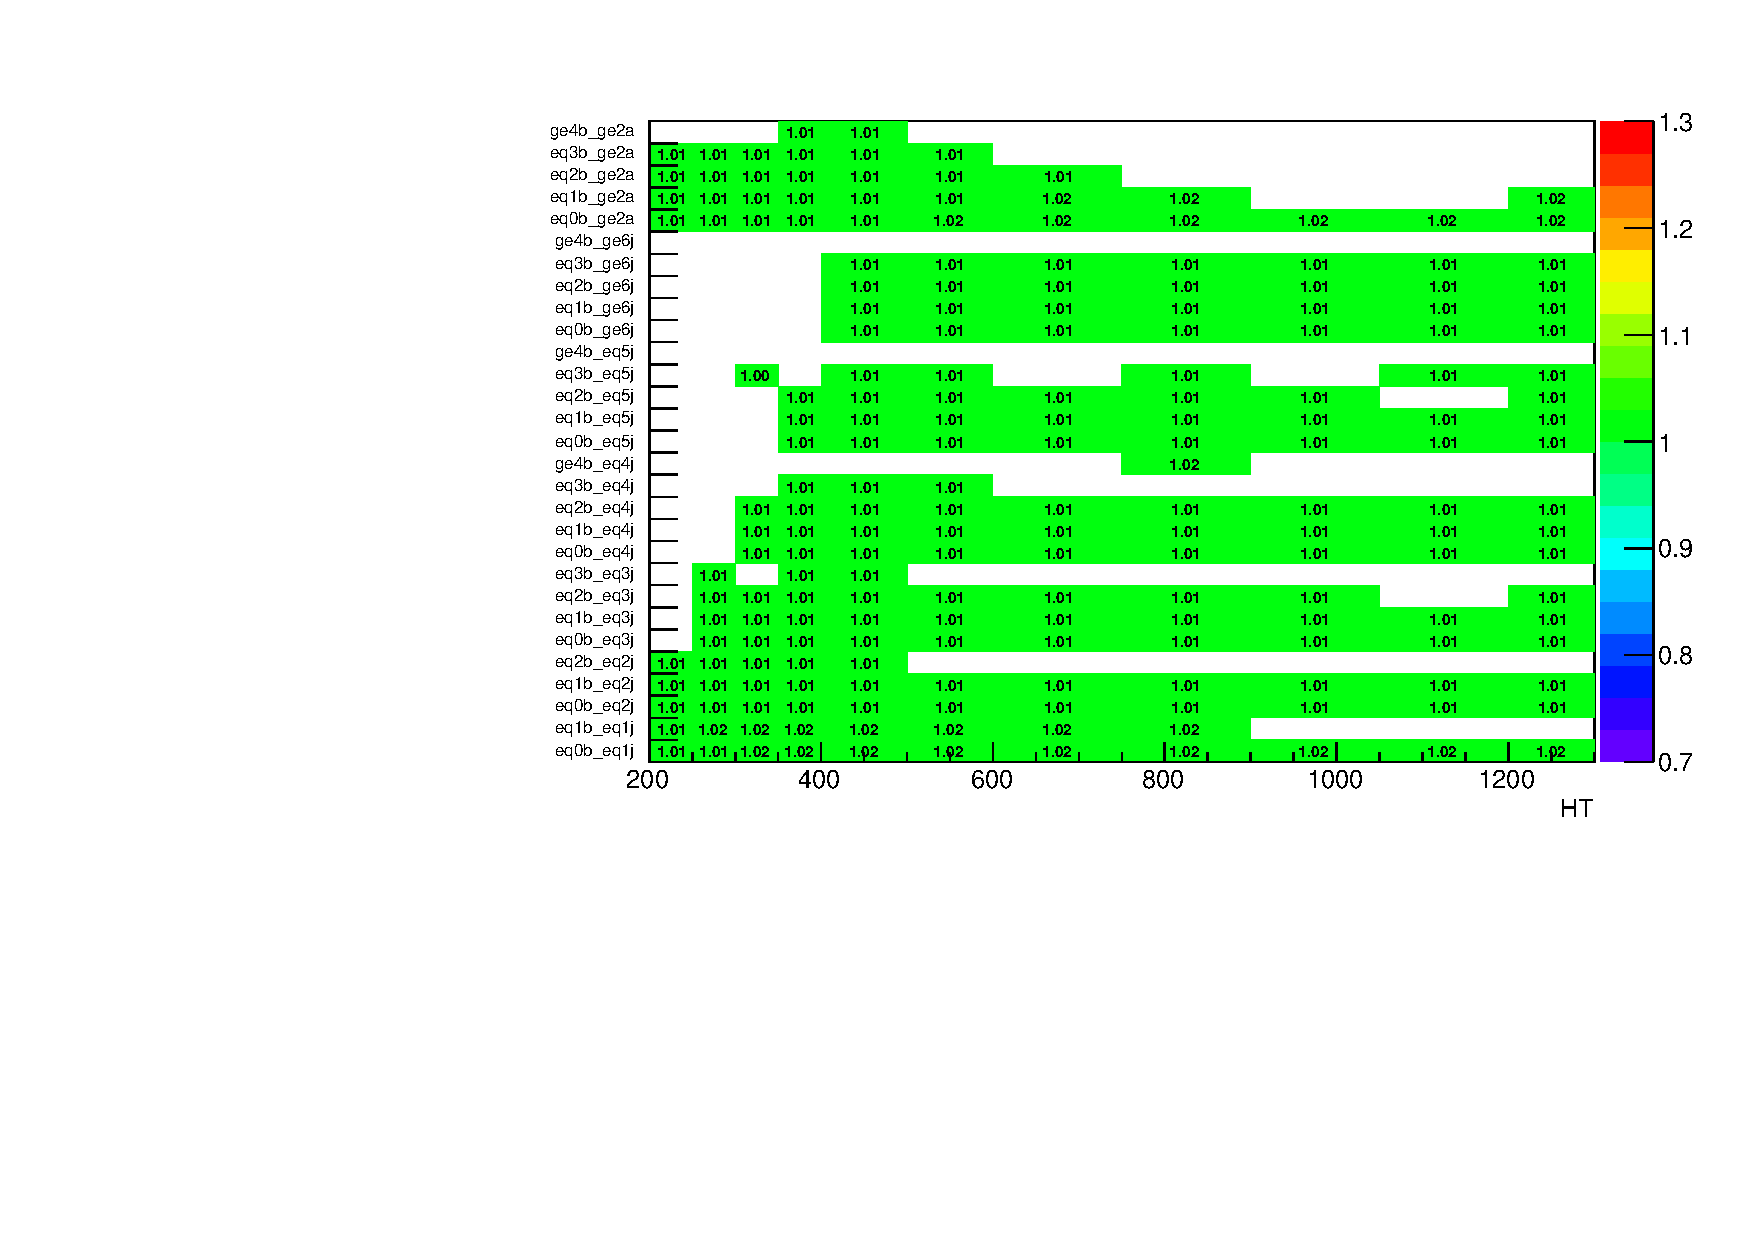
\includegraphics[width=0.5\textwidth]{figures/mcSystematics36p4fb/Ttw/mu/ratiotfh_ht_mht_allmuonSfWeight_Down.pdf}
  }\\

  \caption{\label{fig:tfSyst_muon scale factor_muToTtw} The relative change in the $\mj \rightarrow \mathrm{tt+W}$ transfer
  factors when varying muon scale factor in MC within its uncertainties, as a function of \scalht and jet category. 
  Variations corresponding to $+1\sigma$ ($-1\sigma$) are shown in the left (right) figure. 
  }
\end{figure}

%\clearpage
%\subsection{Photon trigger uncertainty}
%
%\begin{figure}[!h]
%  \centering
%  \subfigure[Photon trigger weight up variation]{
%    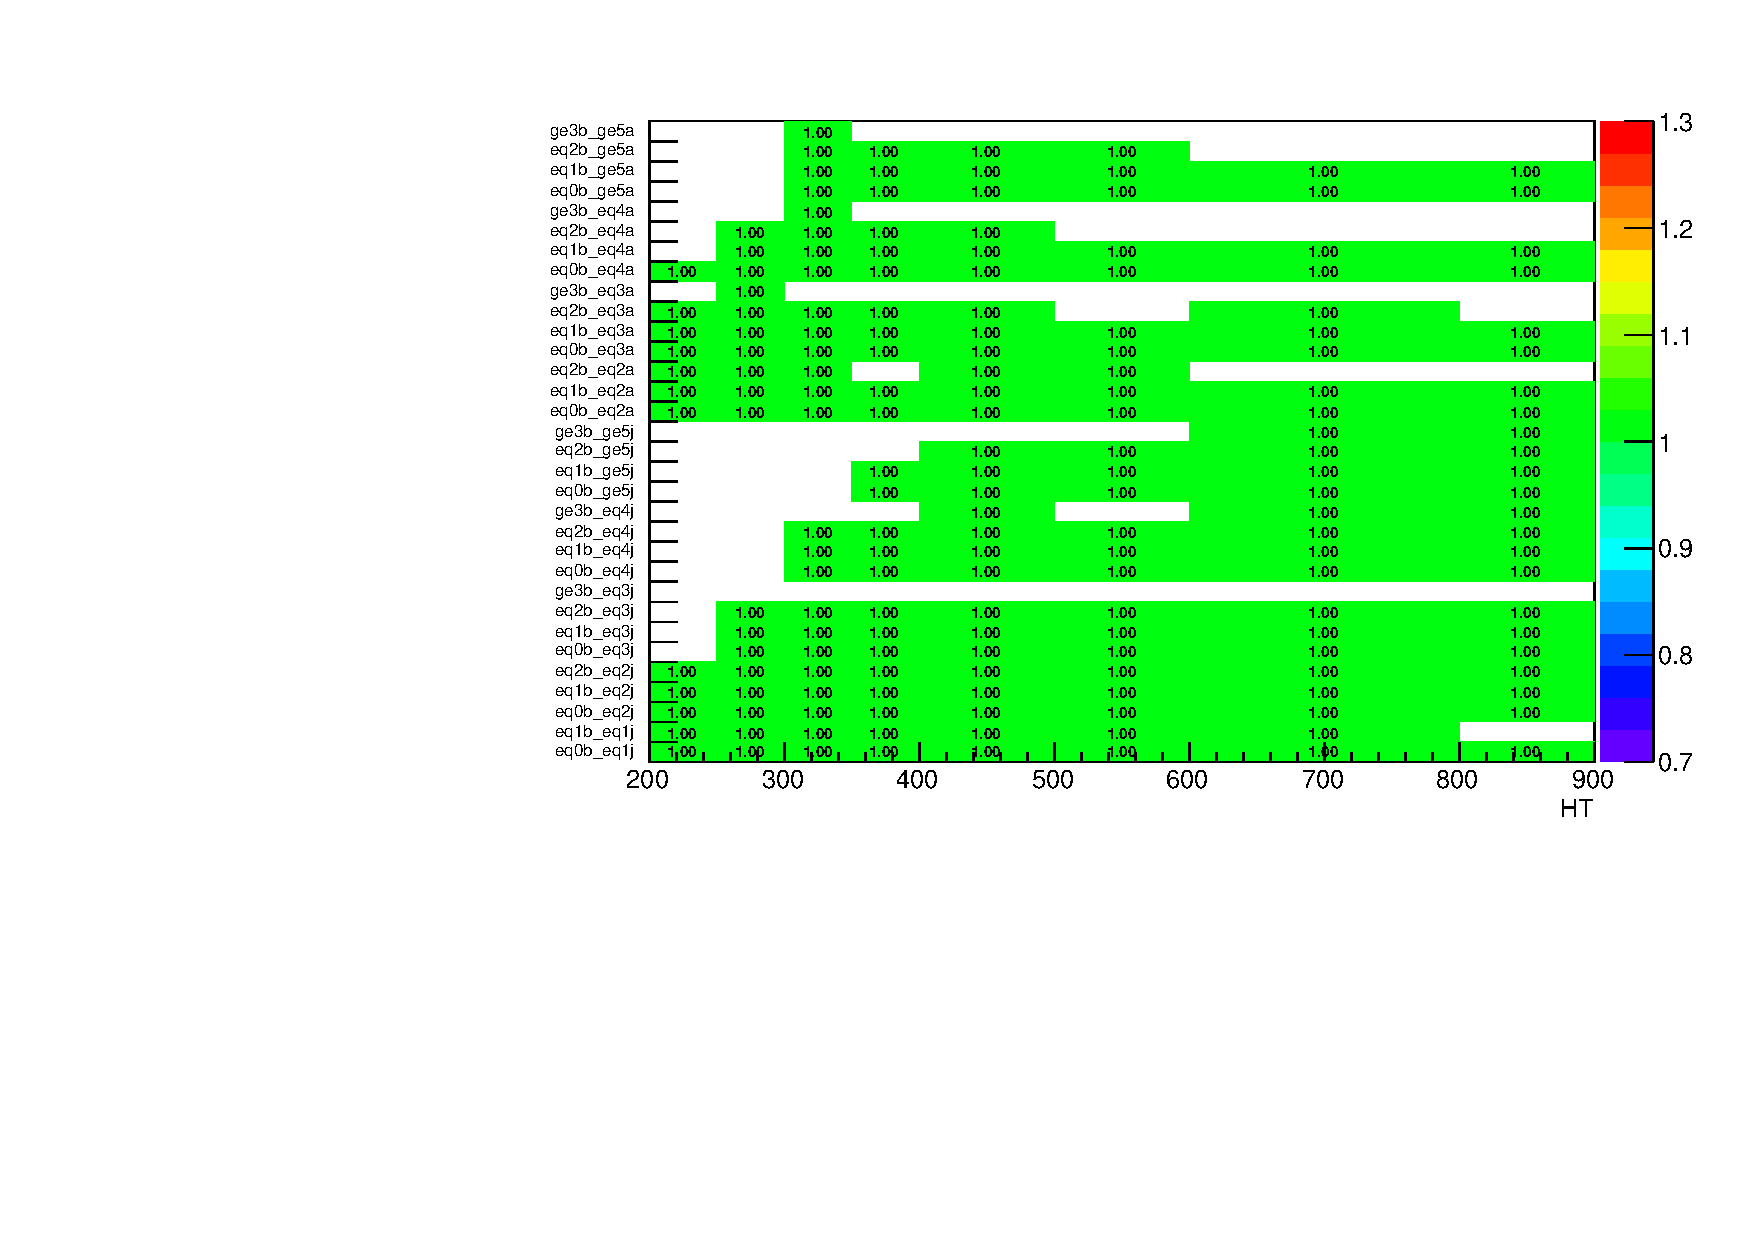
\includegraphics[width=0.5\textwidth]{figures/mcSystematics36p4fb/Zinv/gj/ratiotfh_ht_mht_allphotonTriggerWeight_Up.pdf}
%  } ~~
%  \subfigure[Photon trigger weight down variation]{
%    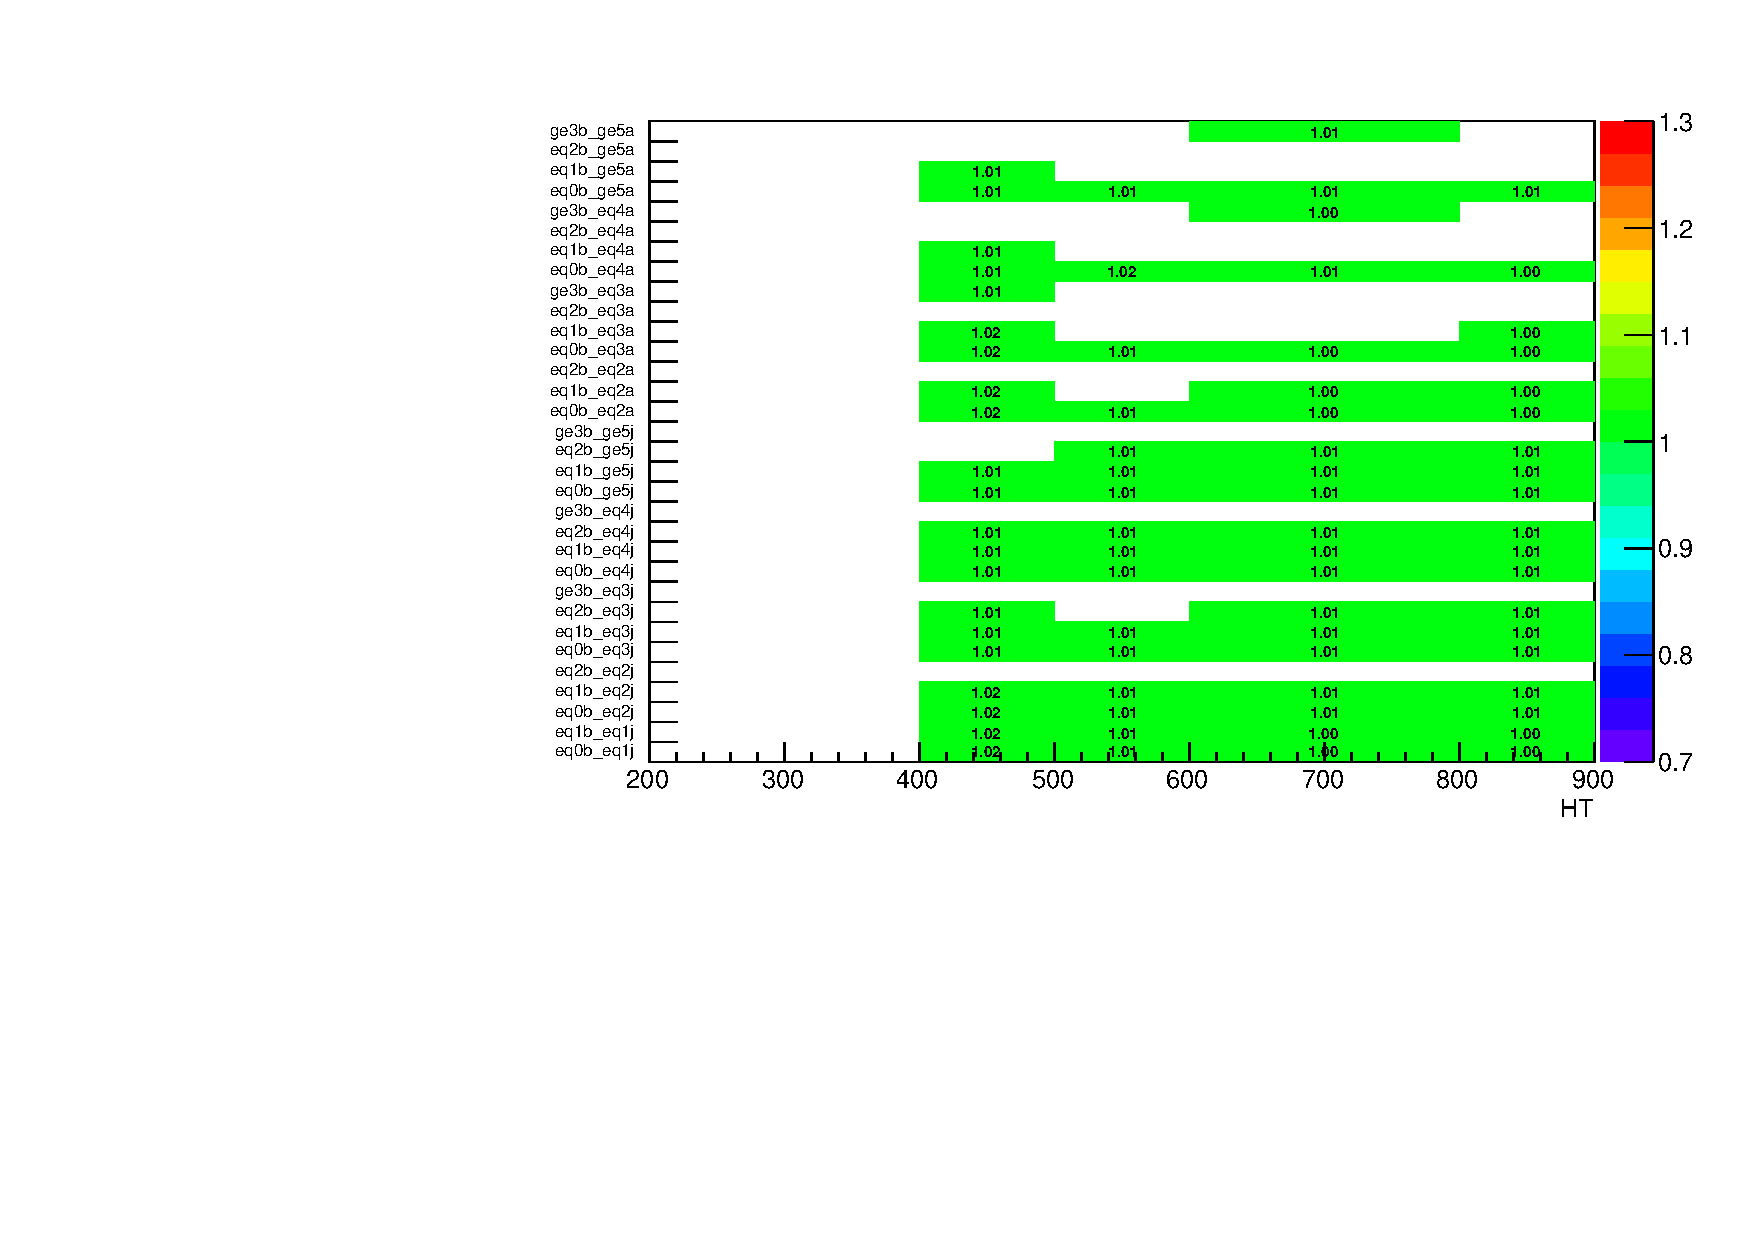
\includegraphics[width=0.5\textwidth]{figures/mcSystematics36p4fb/Zinv/gj/ratiotfh_ht_mht_allphotonTriggerWeight_Down.pdf}
%  }\\
%
%  \caption{\label{fig:tfSyst_photonTrigger_gjToZinv} The relative change in
%  the $\gj \rightarrow (\znunu)$ transfer
%  factors when varying photon trigger weight in MC within its uncertainties, as a function of \scalht and jet category. 
%  Variations corresponding to $+1\sigma$ ($-1\sigma$) are shown in the left (right) figure. 
%  }
%\end{figure}

\clearpage
\subsection{Signal trigger uncertainty}

\begin{figure}[!h]
  \centering
  \subfigure[trigger weight up variation]{
    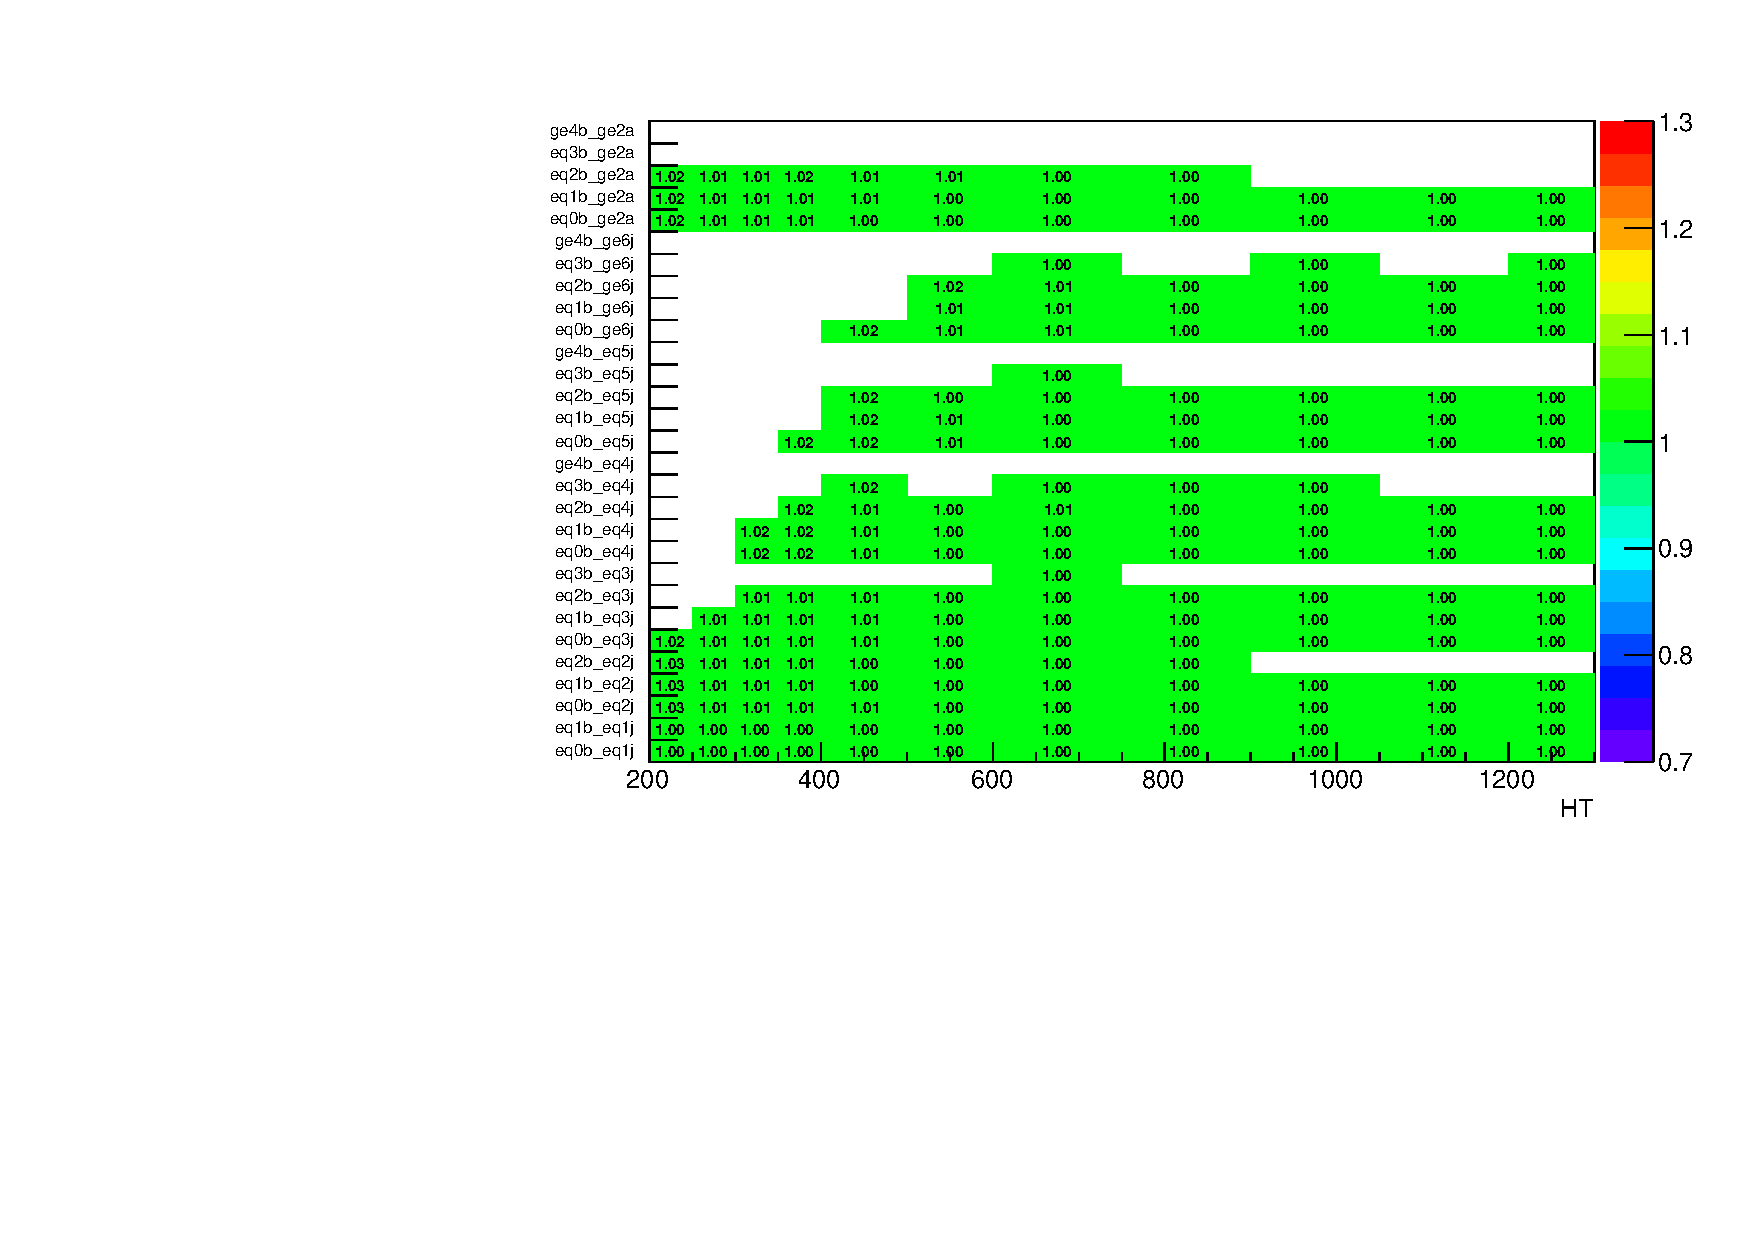
\includegraphics[width=0.5\textwidth]{figures/mcSystematics36p4fb/Zinv/mu/ratiotfh_ht_mht_alltriggerWeight_Up.pdf}
  } ~~
  \subfigure[trigger weight down variation]{
    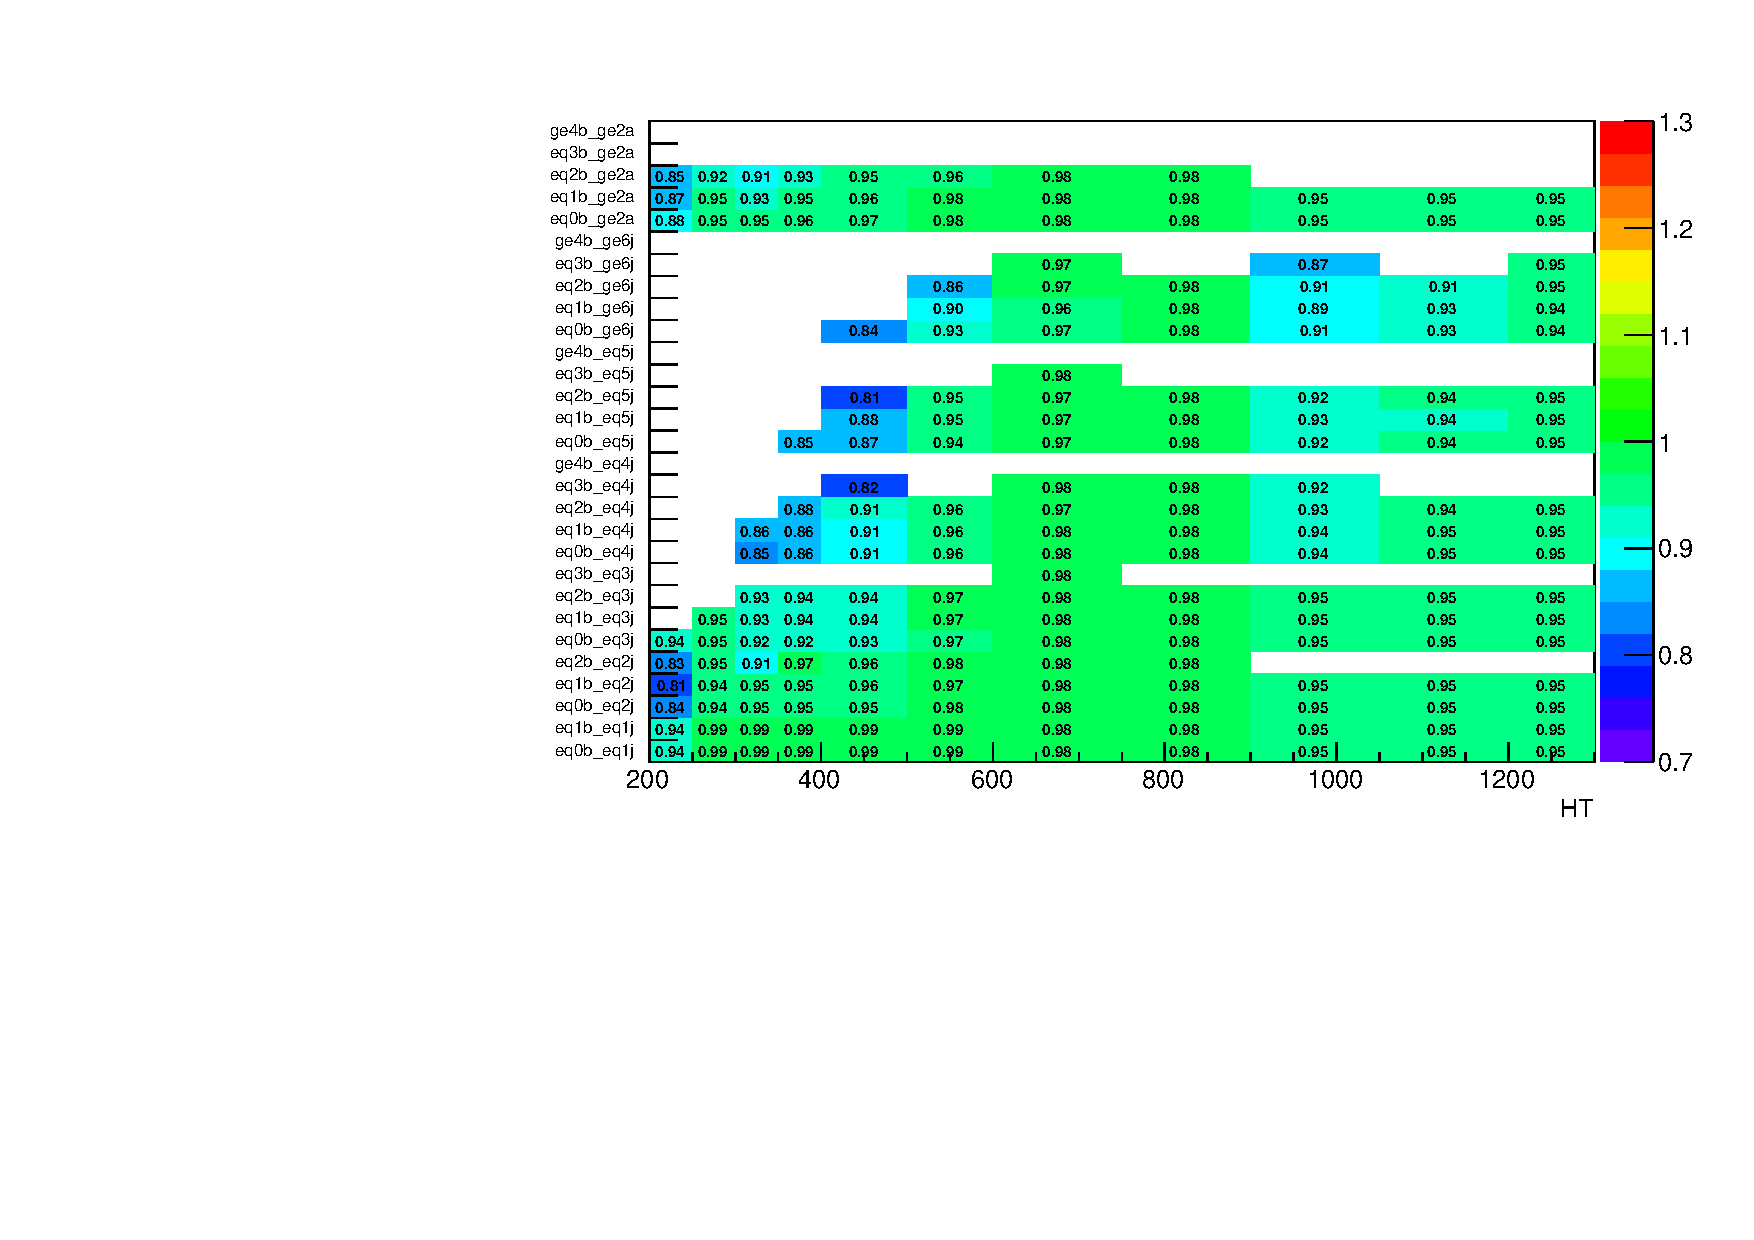
\includegraphics[width=0.5\textwidth]{figures/mcSystematics36p4fb/Zinv/mu/ratiotfh_ht_mht_alltriggerWeight_Down.pdf}
  }\\

  \caption{\label{fig:tfSyst_trigger_muToZinv} The relative change in
  the $\mj \rightarrow (\znunu)$ transfer
  factors when varying trigger weight in MC within its uncertainties, as a function of \scalht and jet category. 
  Variations corresponding to $+1\sigma$ ($-1\sigma$) are shown in the left (right) figure. 
  }
\end{figure}
\begin{figure}[!h]
  \centering
  \subfigure[trigger weight up variation]{
    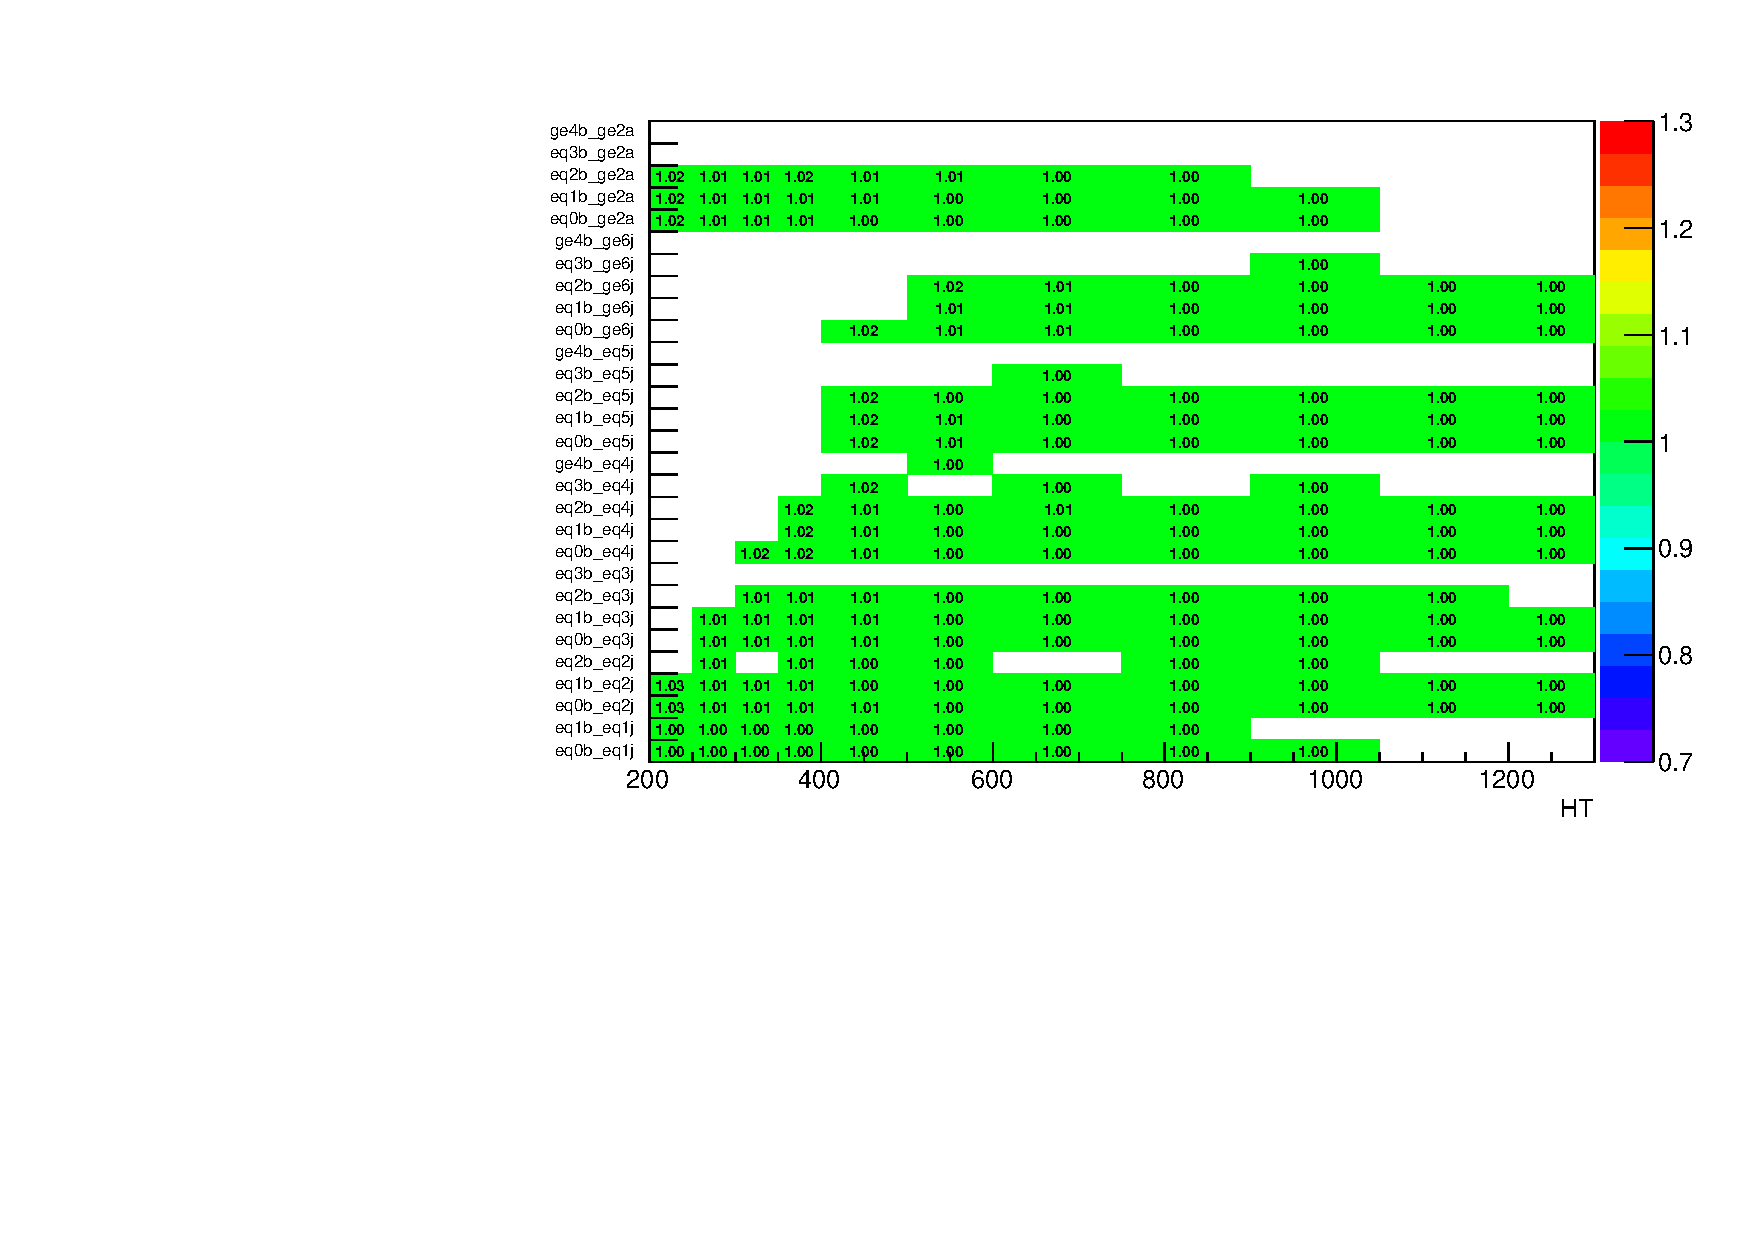
\includegraphics[width=0.5\textwidth]{figures/mcSystematics36p4fb/Zinv/mumu/ratiotfh_ht_mht_alltriggerWeight_Up.pdf}
  } ~~
  \subfigure[trigger weight down variation]{
    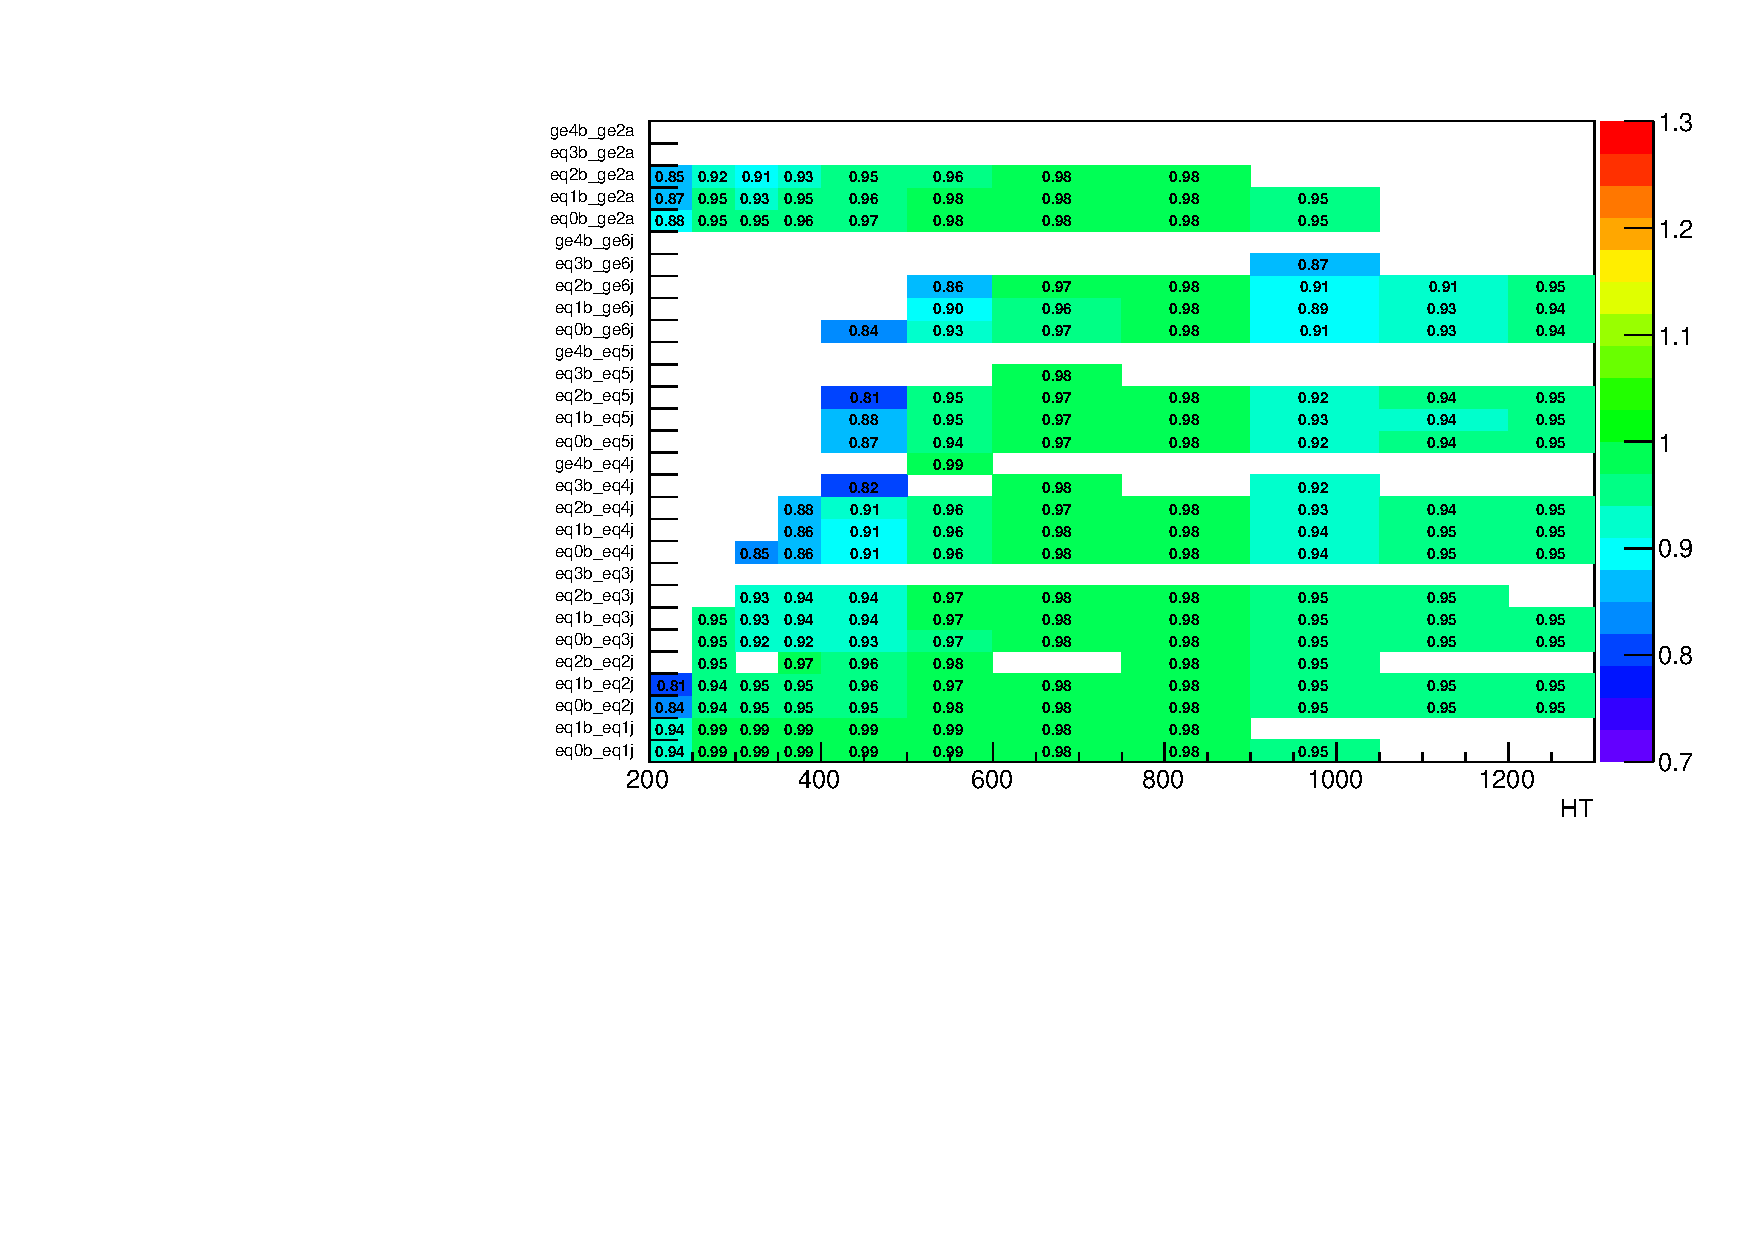
\includegraphics[width=0.5\textwidth]{figures/mcSystematics36p4fb/Zinv/mumu/ratiotfh_ht_mht_alltriggerWeight_Down.pdf}
  }\\

  \caption{\label{fig:tfSyst_trigger_mumuToZinv} The relative change in
  the $\mmj \rightarrow (\znunu)$ transfer
  factors when varying trigger weight in MC within its uncertainties, as a function of \scalht and jet category. 
  Variations corresponding to $+1\sigma$ ($-1\sigma$) are shown in the left (right) figure. 
  }
\end{figure}

\begin{figure}[!h]
  \centering
  \subfigure[trigger weight up variation]{
    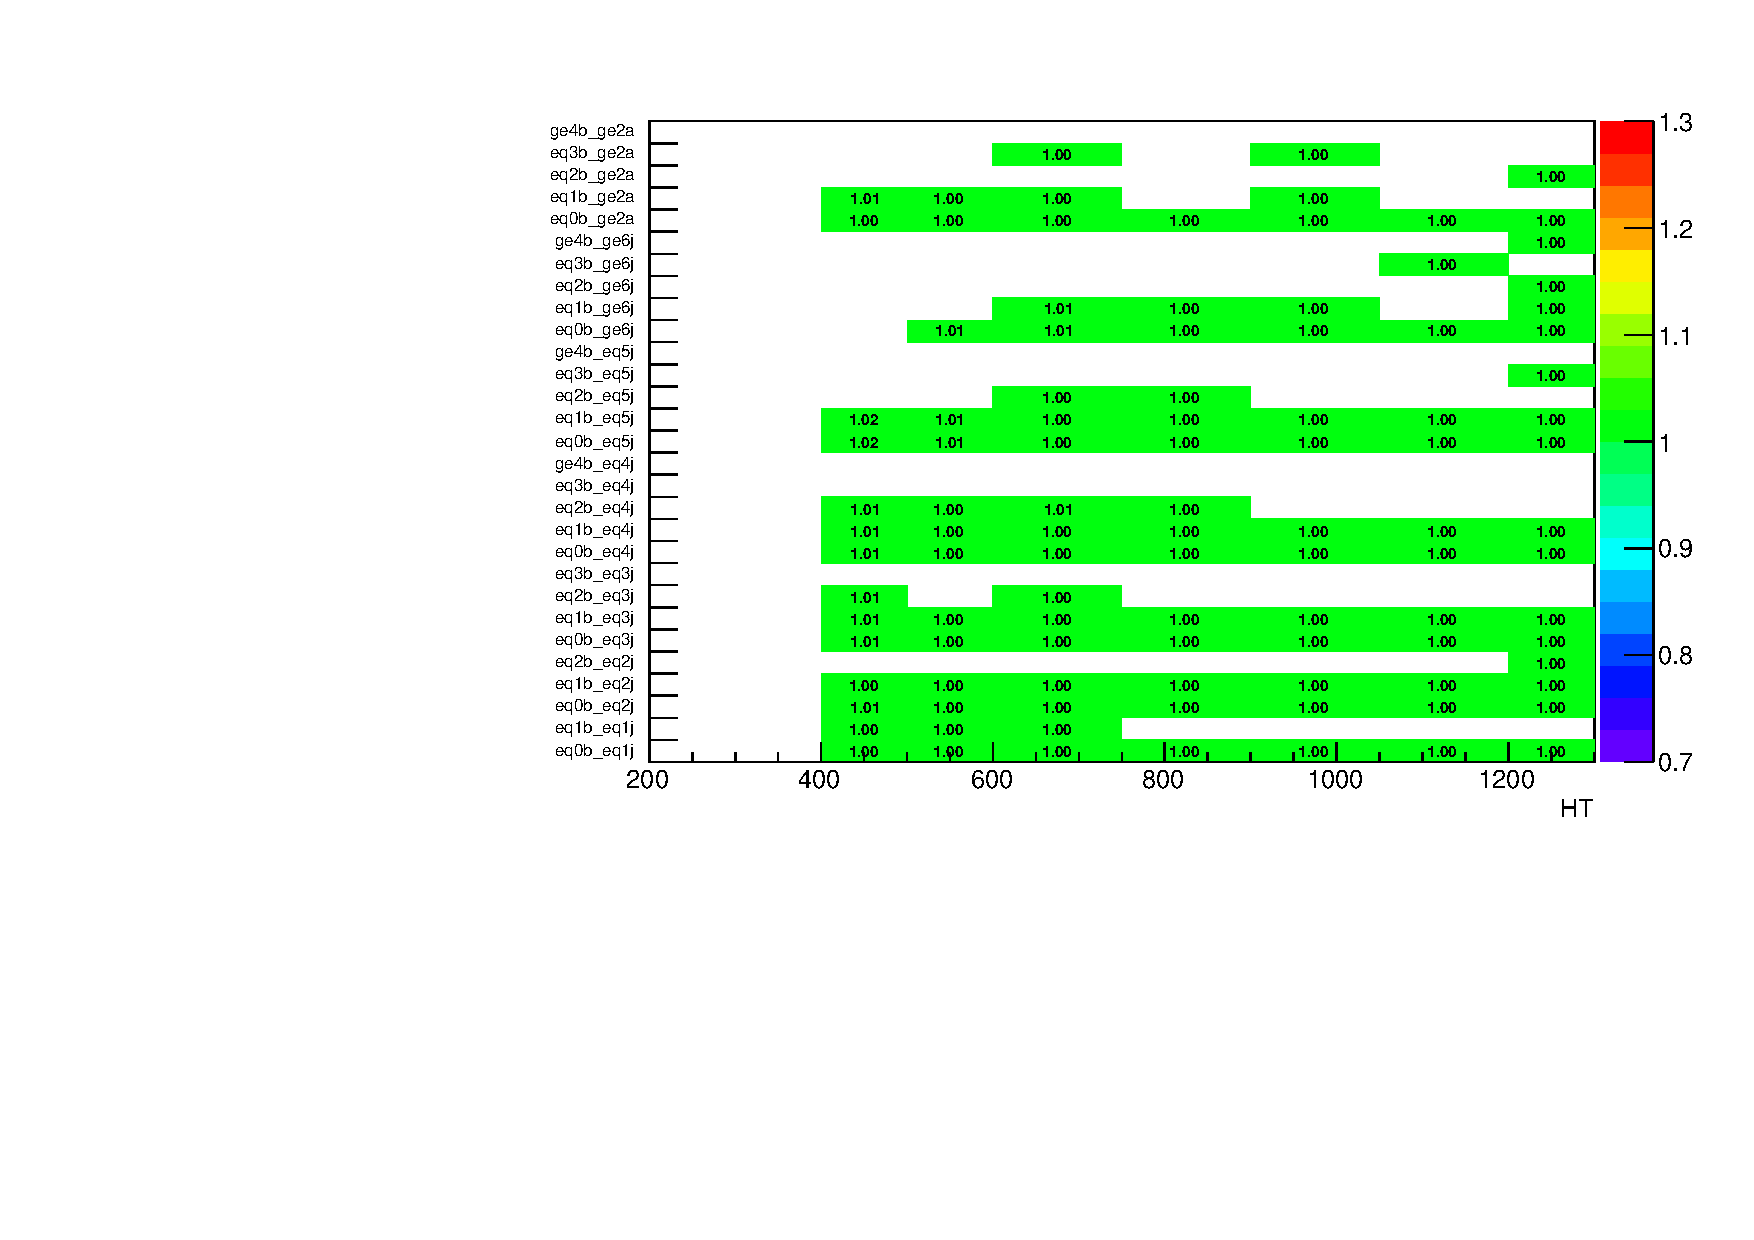
\includegraphics[width=0.5\textwidth]{figures/mcSystematics36p4fb/Zinv/gj/ratiotfh_ht_mht_alltriggerWeight_Up.pdf}
  } ~~
  \subfigure[trigger weight down variation]{
    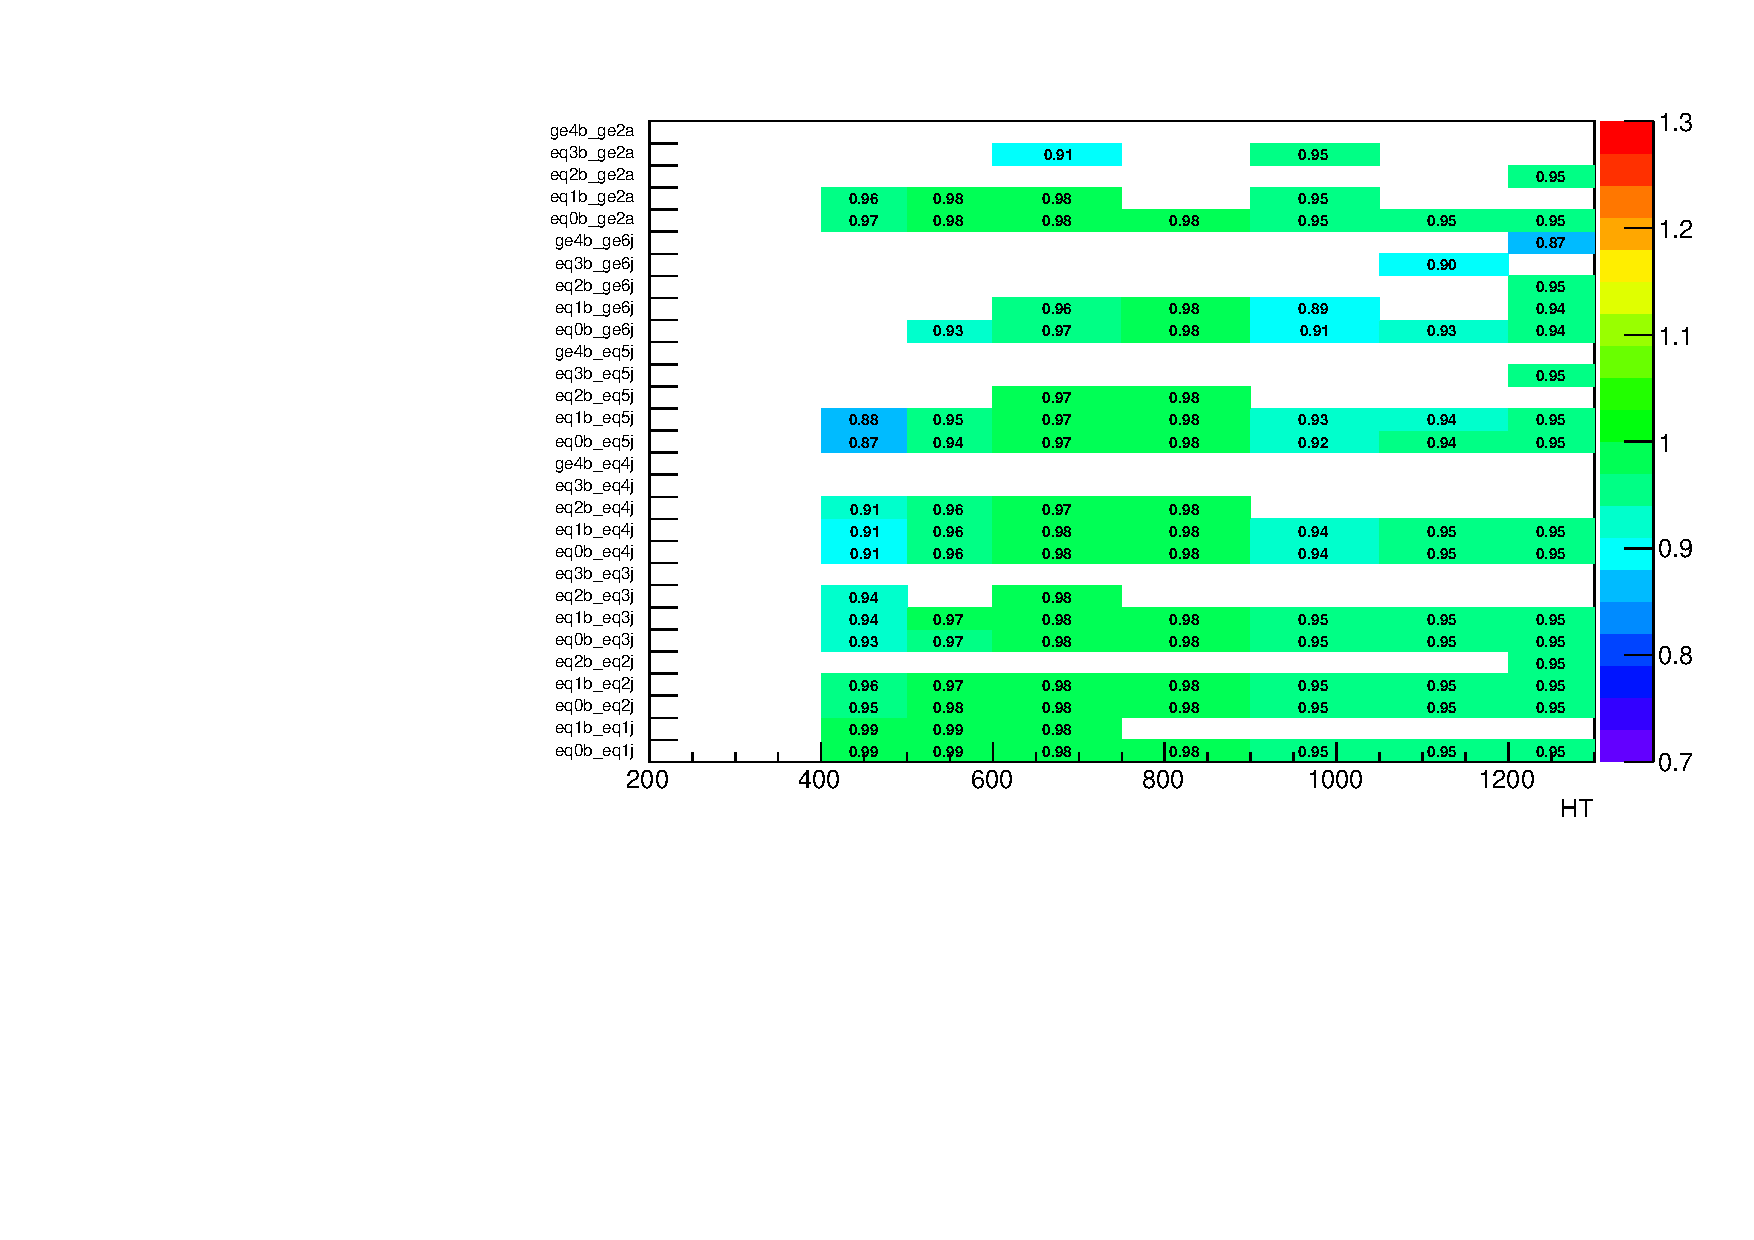
\includegraphics[width=0.5\textwidth]{figures/mcSystematics36p4fb/Zinv/gj/ratiotfh_ht_mht_alltriggerWeight_Down.pdf}
  }\\

  \caption{\label{fig:tfSyst_trigger_gjToZinv} The relative change in
  the $\gj \rightarrow (\znunu)$ transfer
  factors when varying trigger weight in MC within its uncertainties, as a function of \scalht and jet category. 
  Variations corresponding to $+1\sigma$ ($-1\sigma$) are shown in the left (right) figure. 
  }
\end{figure}

\begin{figure}[!h]
  \centering
  \subfigure[trigger weight up variation]{
    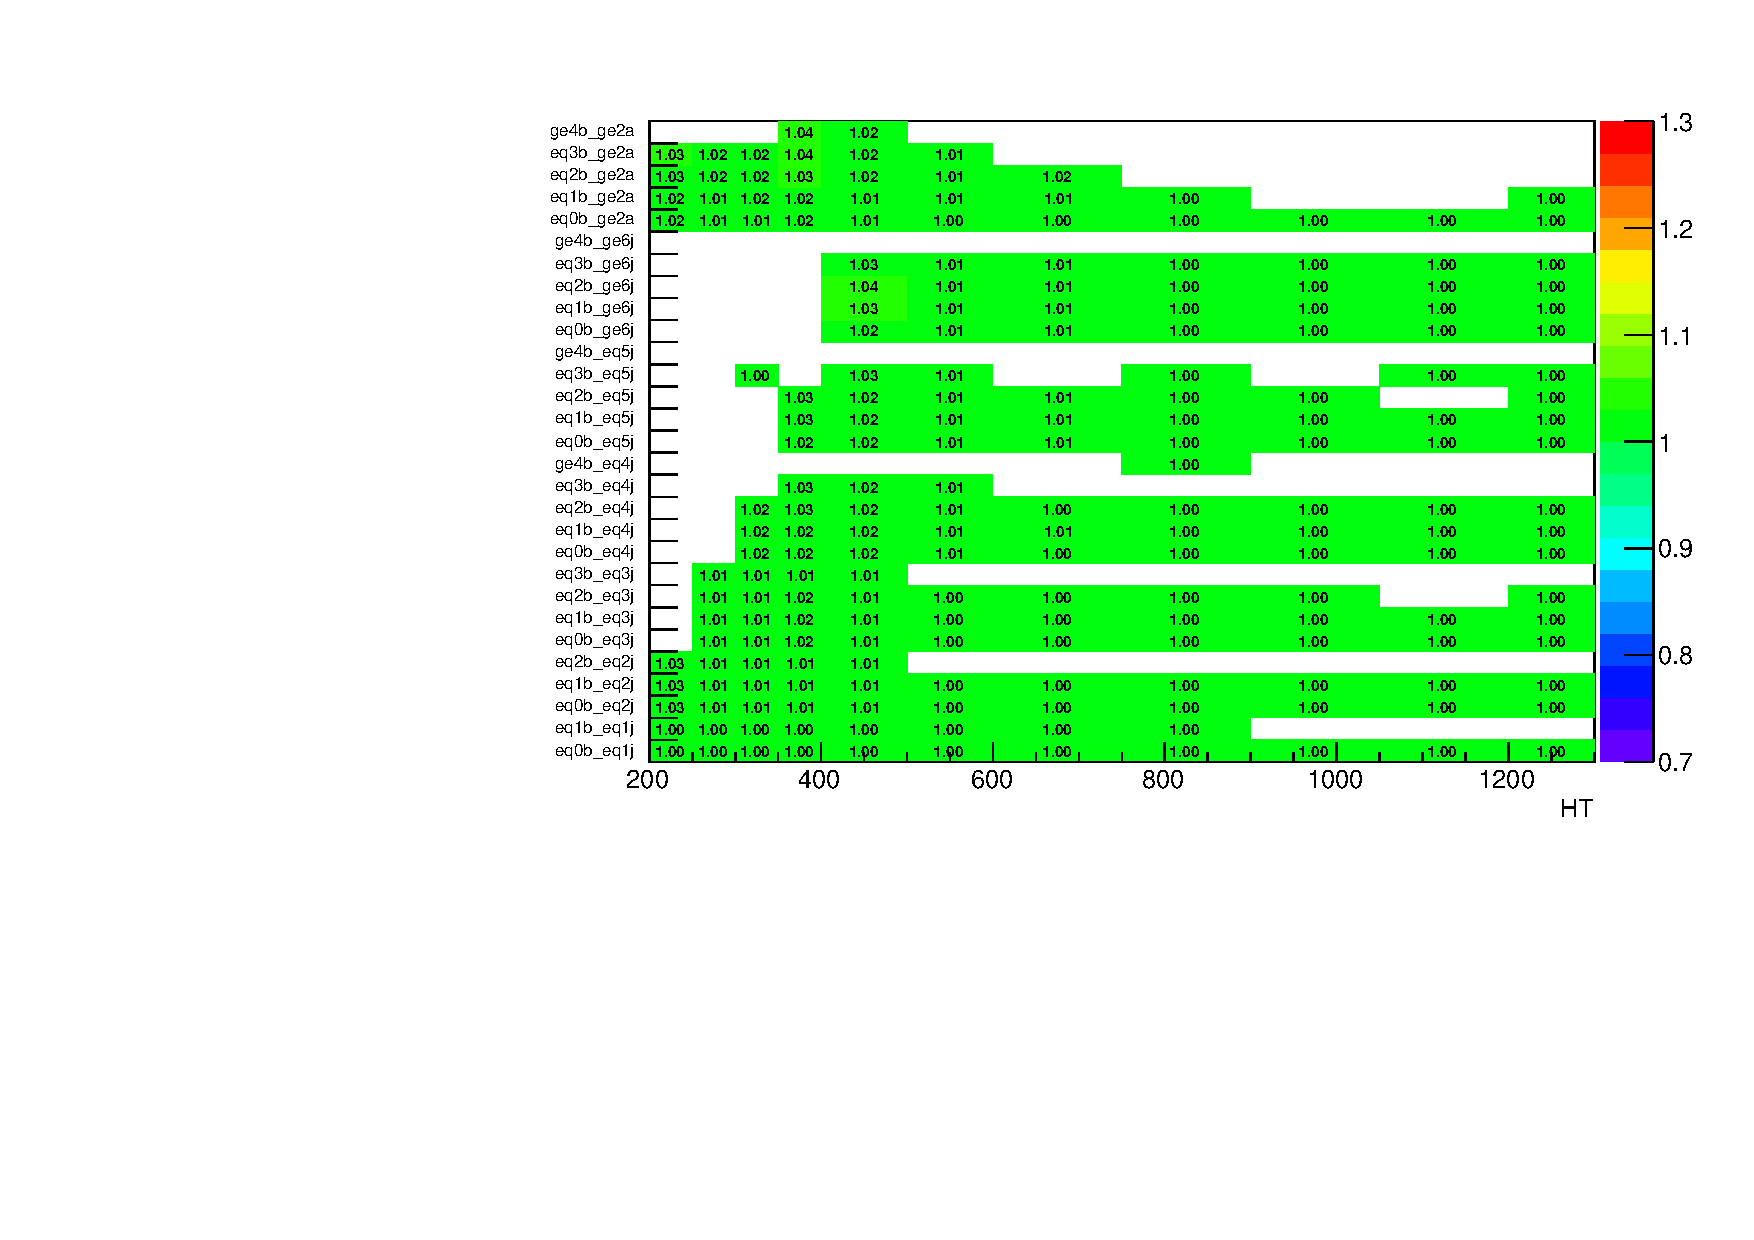
\includegraphics[width=0.5\textwidth]{figures/mcSystematics36p4fb/Ttw/mu/ratiotfh_ht_mht_alltriggerWeight_Up.pdf}
  } ~~
  \subfigure[trigger weight down variation]{
    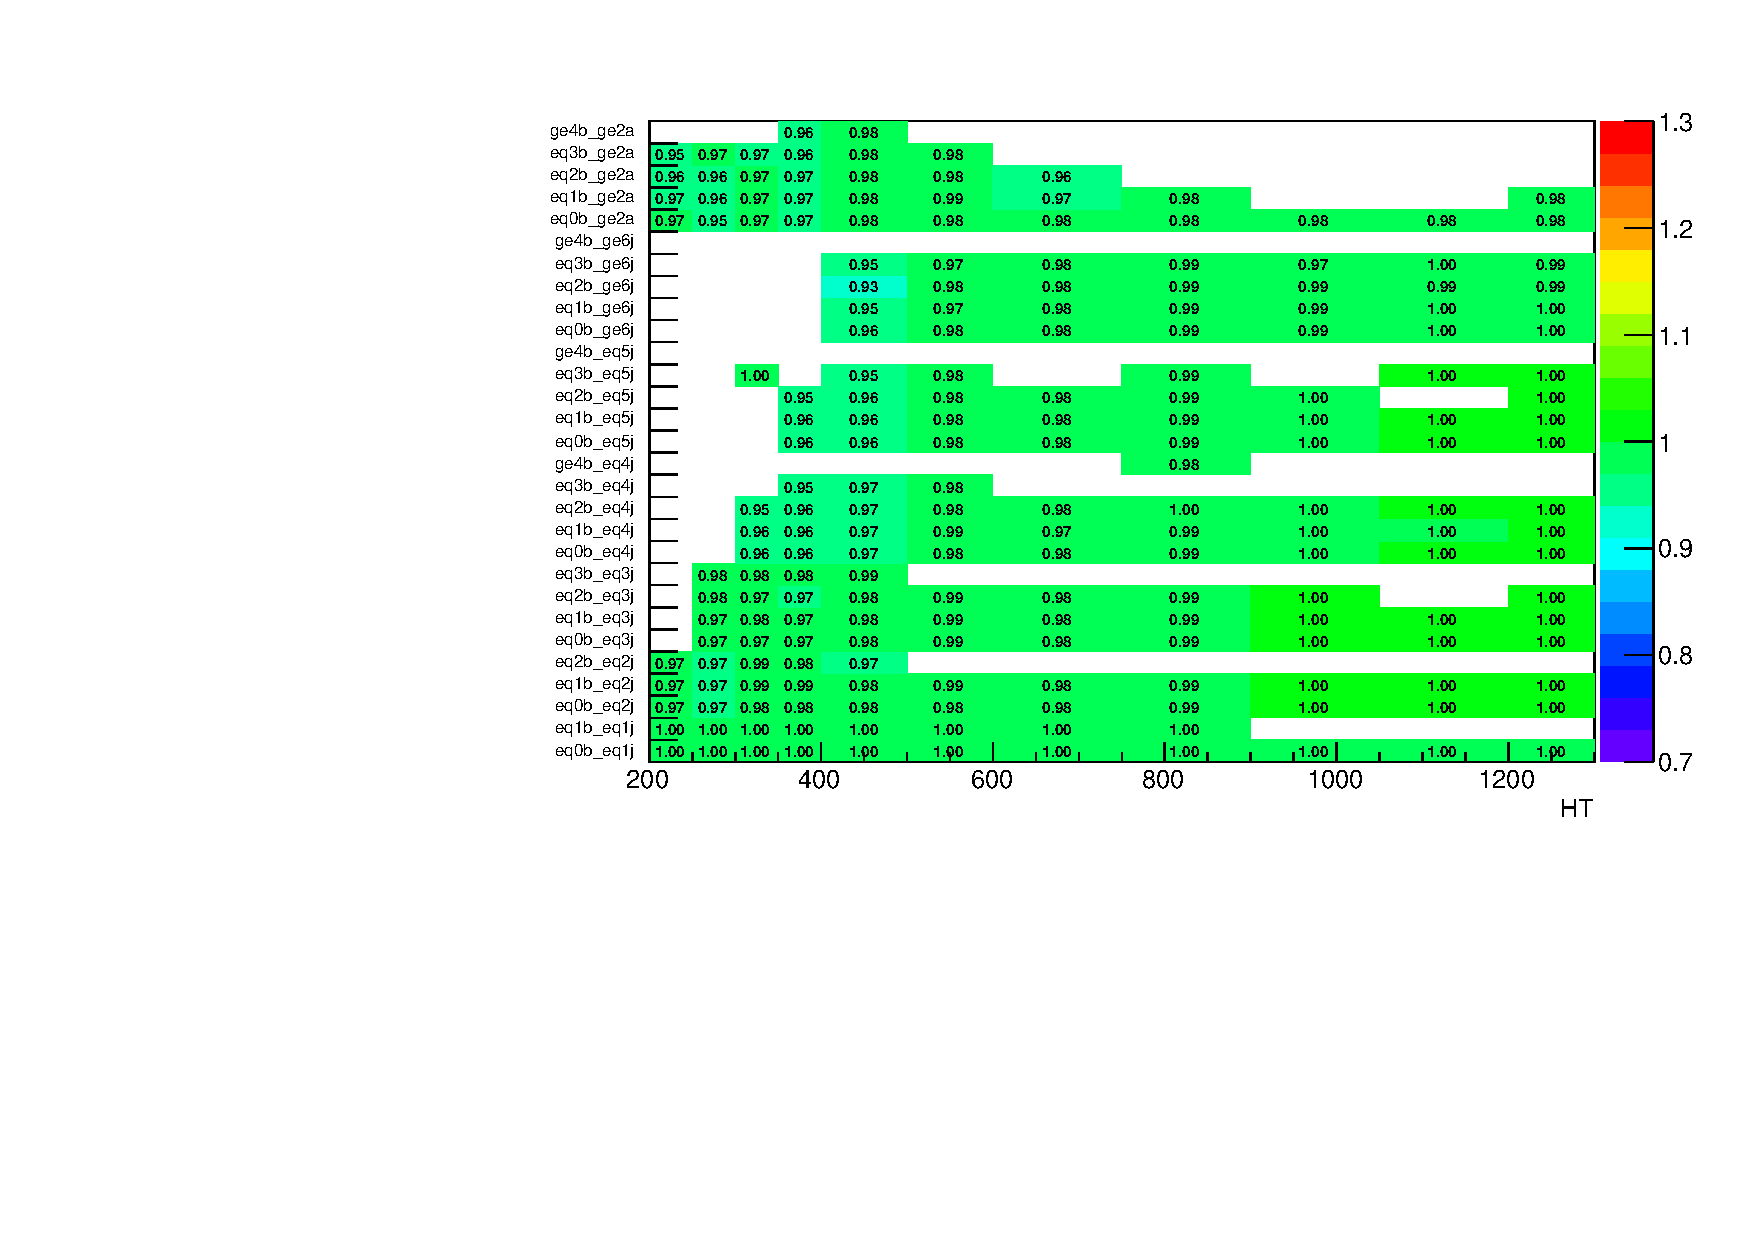
\includegraphics[width=0.5\textwidth]{figures/mcSystematics36p4fb/Ttw/mu/ratiotfh_ht_mht_alltriggerWeight_Down.pdf}
  }\\

  \caption{\label{fig:tfSyst_trigger_muToTtw} The relative change in the $\mj \rightarrow \mathrm{tt+W}$ transfer
  factors when varying trigger weight in MC within its uncertainties, as a function of \scalht and jet category. 
  Variations corresponding to $+1\sigma$ ($-1\sigma$) are shown in the left (right) figure. 
  }
\end{figure}

%\subsection{Top $p_T$ reweighting}
%
%\begin{figure}[!h]
%  \centering
%  \subfigure[top $p_{T}$ weight up variation]{
%    \includegraphics[width=0.5\textwidth]{figures/mcSystematics36p4fb/Zinv/mu/ratiotfh_ht_mht_alltopPtWeight_Up.pdf}
%  } ~~
%  \subfigure[top $p_{T}$ weight down variation]{
%    \includegraphics[width=0.5\textwidth]{figures/mcSystematics36p4fb/Zinv/mu/ratiotfh_ht_mht_alltopPtWeight_Down.pdf}
%  }\\
%
%  \caption{\label{fig:tfSyst_topPt_muToZinv} The relative change in
%  the $\mj \rightarrow (\znunu)$ transfer
%  factors when varying top $p_{T}$ weight in MC within its uncertainties, as a function of \scalht and jet category. 
%  Variations corresponding to $+1\sigma$ ($-1\sigma$) are shown in the left (right) figure. 
%  }
%\end{figure}
%
%\begin{figure}[!h]
%  \centering
%  \subfigure[top $p_{T}$ weight up variation]{
%    \includegraphics[width=0.5\textwidth]{figures/mcSystematics36p4fb/Zinv/mumu/ratiotfh_ht_mht_alltopPtWeight_Up.pdf}
%  } ~~
%  \subfigure[top $p_{T}$ weight down variation]{
%    \includegraphics[width=0.5\textwidth]{figures/mcSystematics36p4fb/Zinv/mumu/ratiotfh_ht_mht_alltopPtWeight_Down.pdf}
%  }\\
%
%  \caption{\label{fig:tfSyst_topPt_mumuToZinv} The relative change in
%  the $\mmj \rightarrow (\znunu)$ transfer
%  factors when varying top $p_{T}$ weight in MC within its uncertainties, as a function of \scalht and jet category. 
%  Variations corresponding to $+1\sigma$ ($-1\sigma$) are shown in the left (right) figure. 
%  }
%\end{figure}
%
%\begin{figure}[!h]
%  \centering
%  \subfigure[top $p_{T}$ weight up variation]{
%    \includegraphics[width=0.5\textwidth]{figures/mcSystematics36p4fb/Ttw/mu/ratiotfh_ht_mht_alltopPtWeight_Up.pdf}
%  } ~~
%  \subfigure[top $p_{T}$ weight down variation]{
%    \includegraphics[width=0.5\textwidth]{figures/mcSystematics36p4fb/Ttw/mu/ratiotfh_ht_mht_alltopPtWeight_Down.pdf}
%  }\\
%
%  \caption{\label{fig:tfSyst_topPt_muToTtw} The relative change in the $\mj \rightarrow \mathrm{tt+W}$ transfer
%  factors when varying top $p_{T}$ weight in MC within its uncertainties, as a function of \scalht and jet category. 
%  Variations corresponding to $+1\sigma$ ($-1\sigma$) are shown in the left (right) figure. 
%  }
%\end{figure}

\clearpage
\subsection{PU reweighting}

\begin{figure}[!h]
  \centering
  \subfigure[PU weight up variation]{
    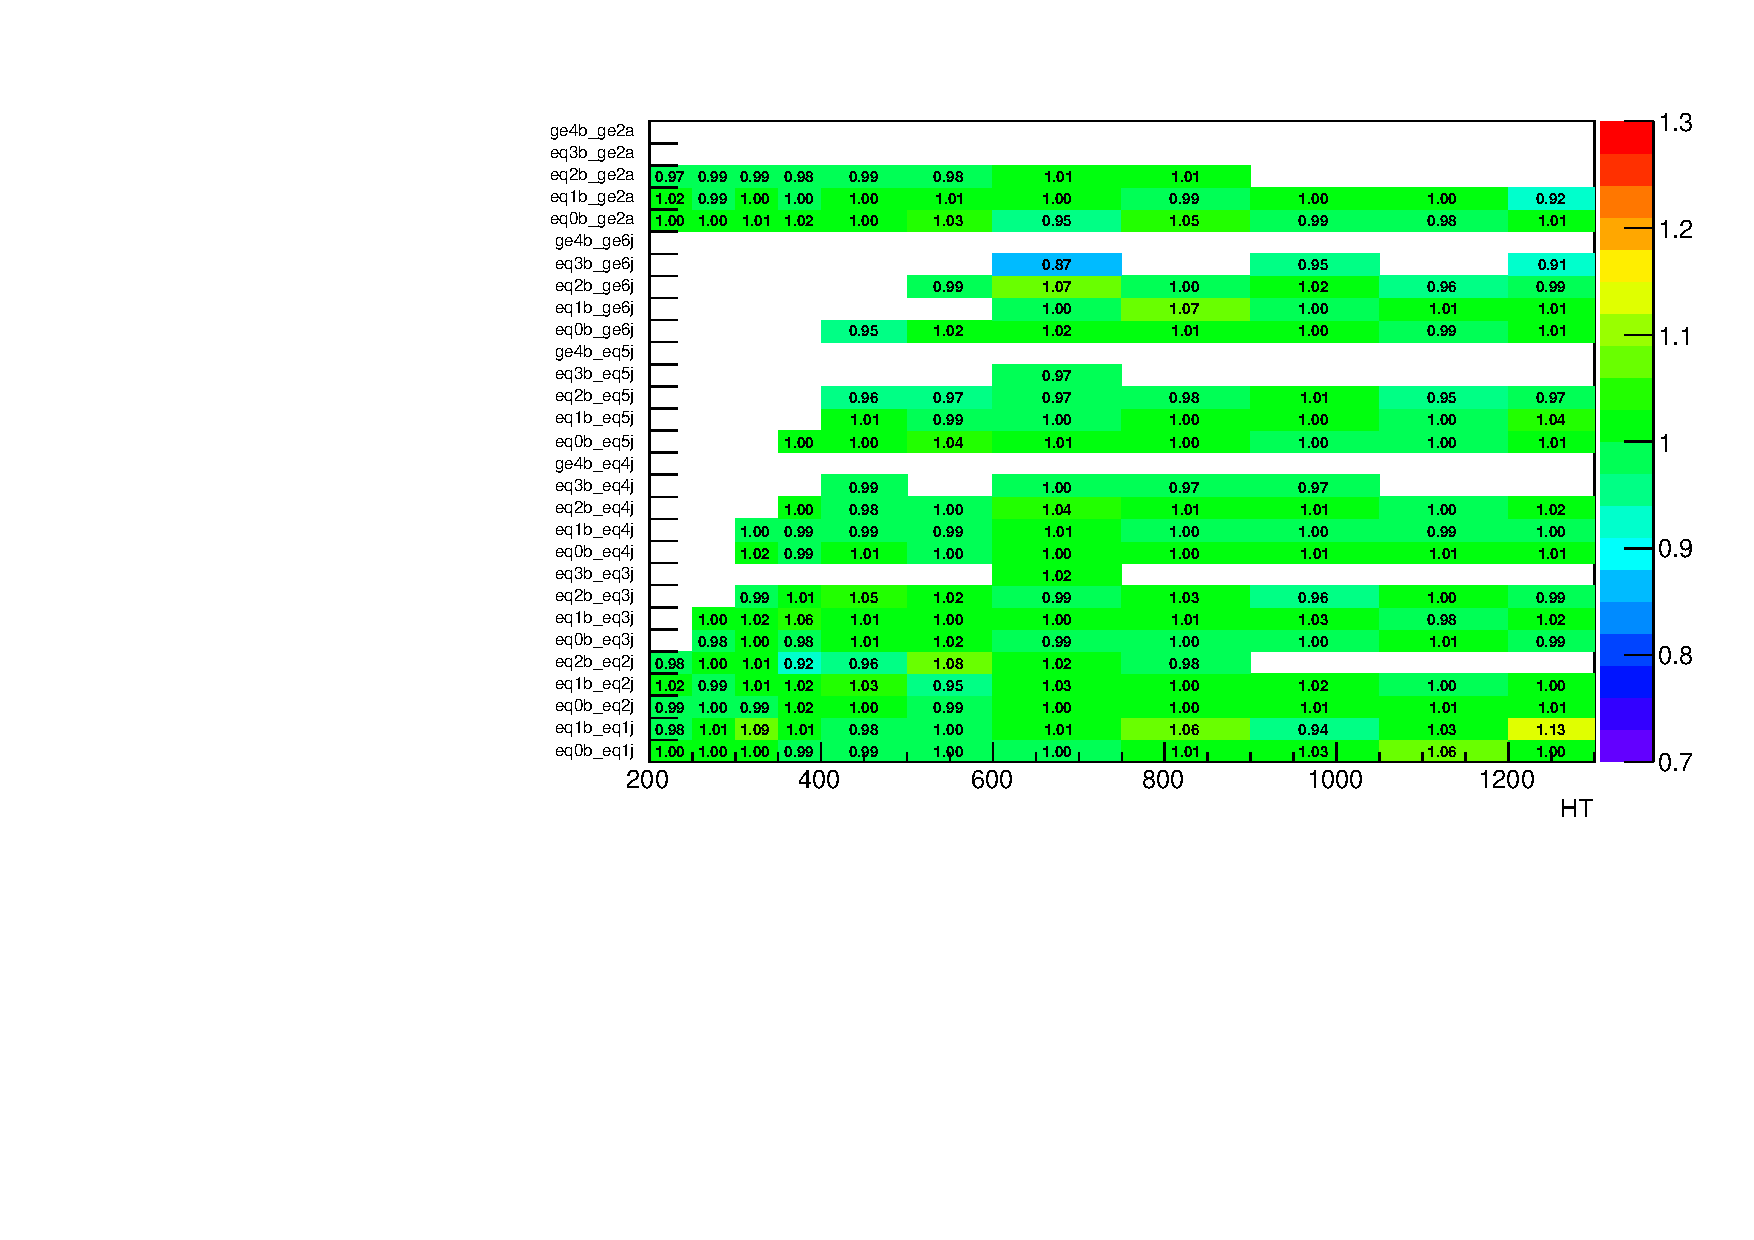
\includegraphics[width=0.5\textwidth]{figures/mcSystematics36p4fb/Zinv/mu/ratiotfh_ht_mht_allpuWeight_Up.pdf}
  } ~~
  \subfigure[PU weight down variation]{
    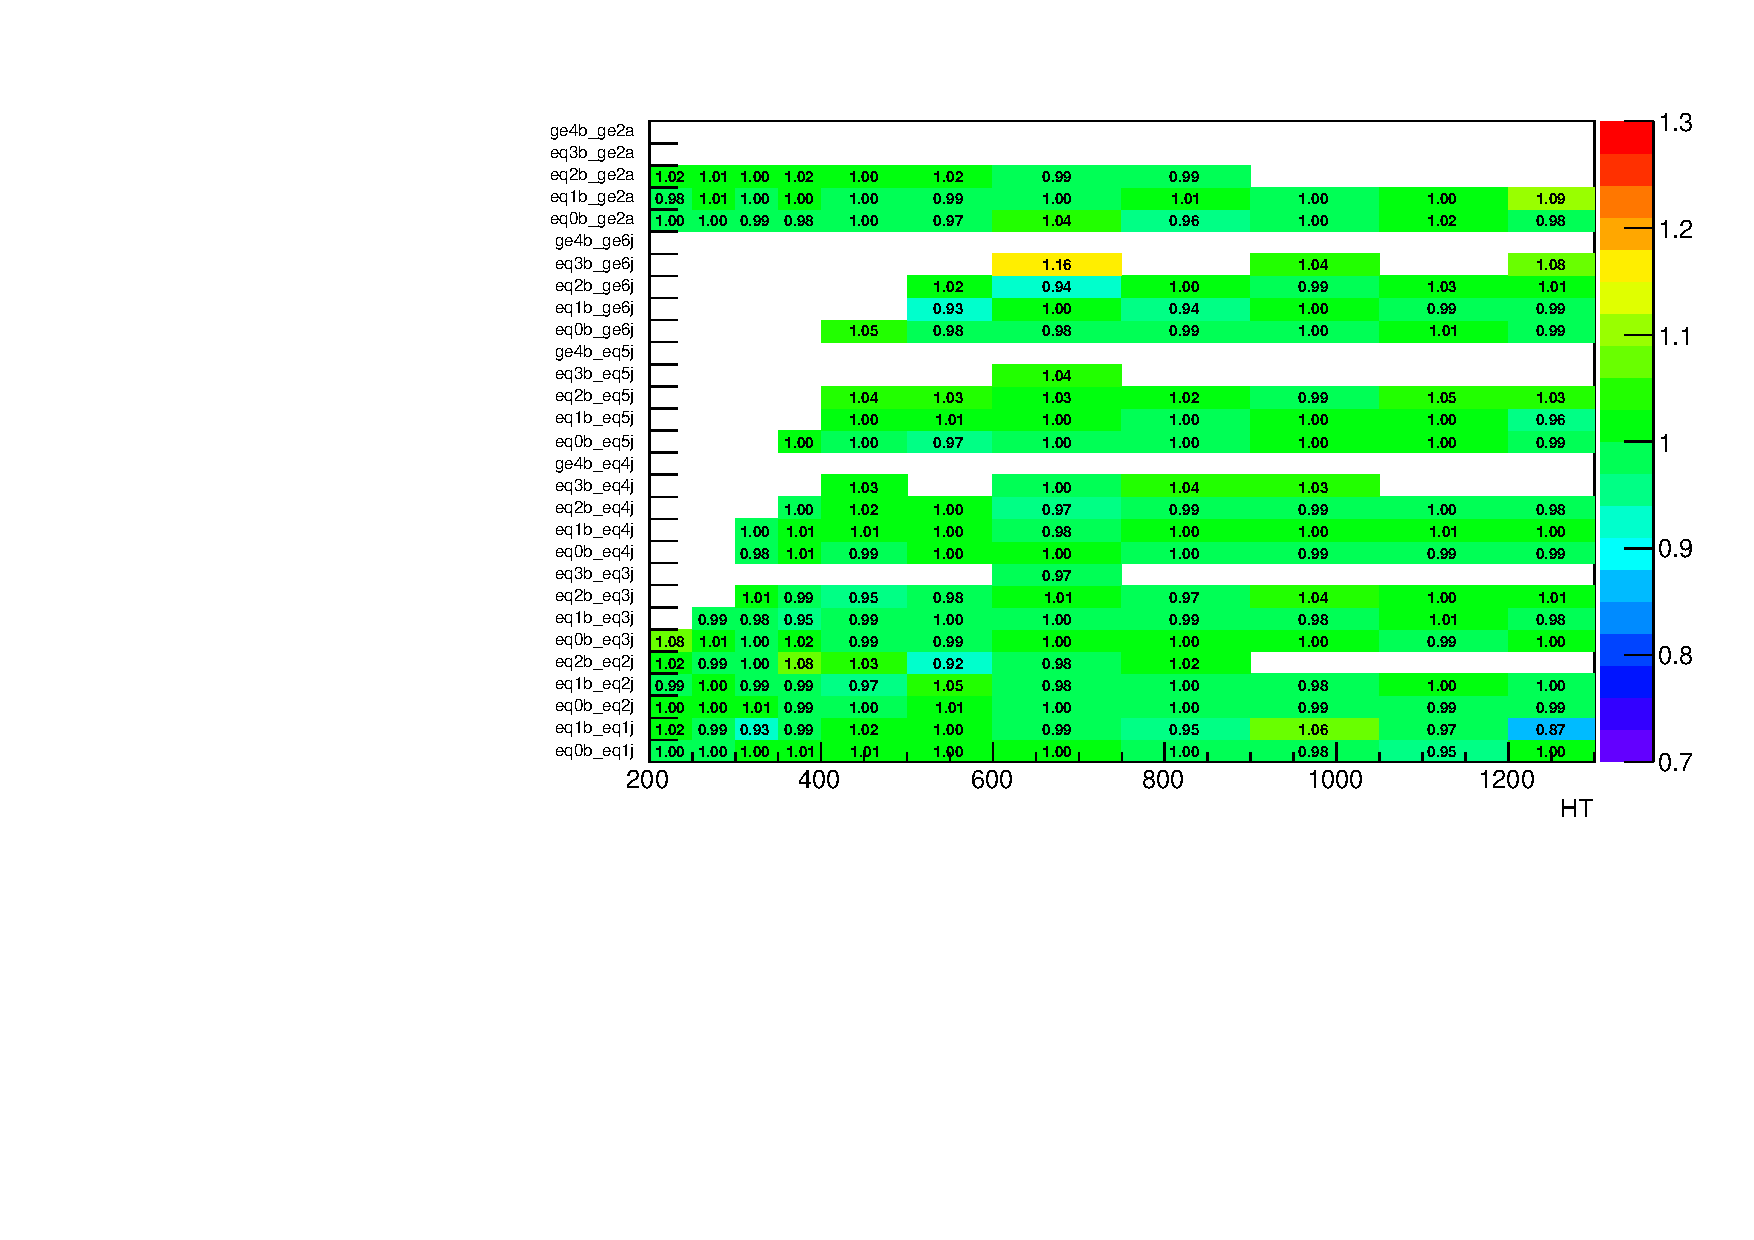
\includegraphics[width=0.5\textwidth]{figures/mcSystematics36p4fb/Zinv/mu/ratiotfh_ht_mht_allpuWeight_Down.pdf}
  }\\

  \caption{\label{fig:tfSyst_pu_muToZinv} The relative change in the
  $\mj \rightarrow (\znunu)$ transfer
  factors when varying PU weight in MC within its uncertainties, as a function of \scalht and jet category. 
  Variations corresponding to $+1\sigma$ ($-1\sigma$) are shown in the left (right) figure. 
  }
\end{figure}

\begin{figure}[!h]
  \centering
  \subfigure[PU weight up variation]{
    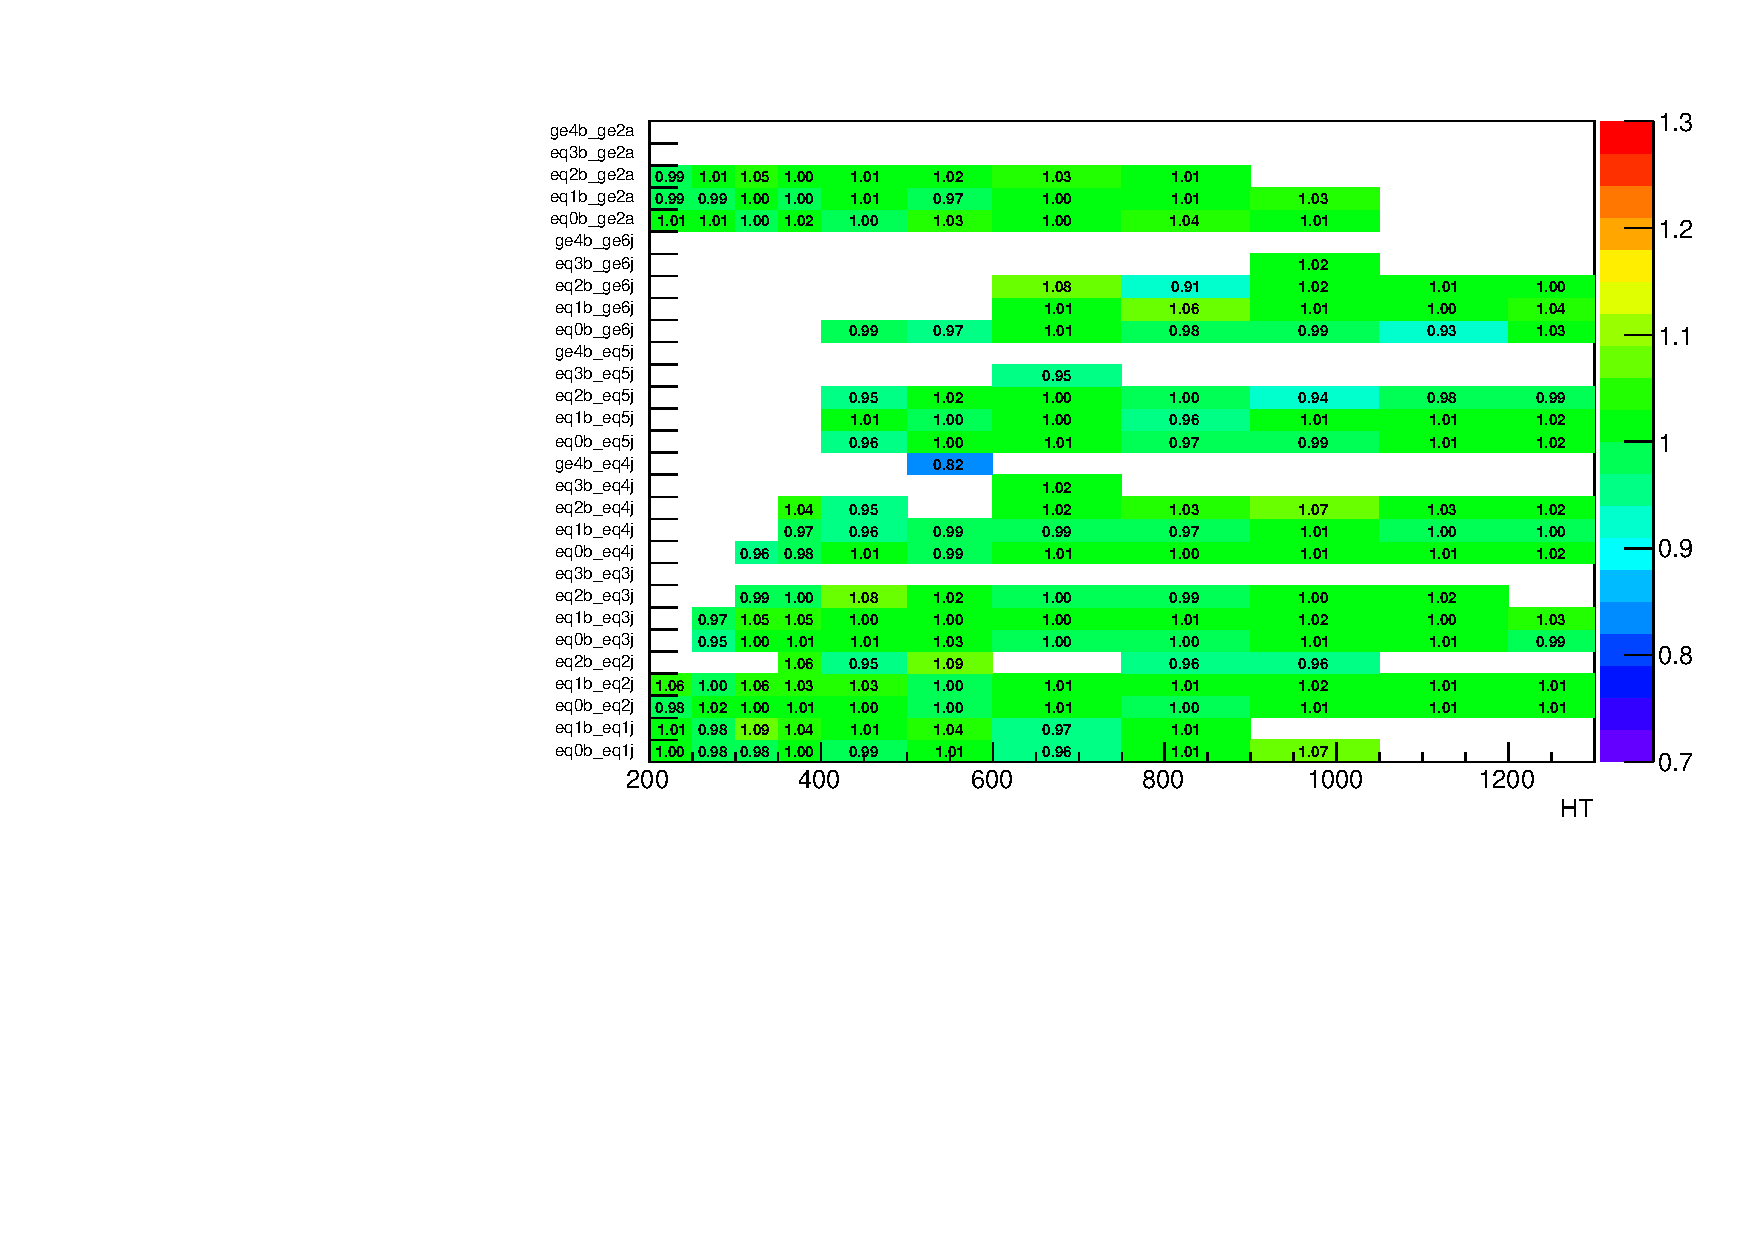
\includegraphics[width=0.5\textwidth]{figures/mcSystematics36p4fb/Zinv/mumu/ratiotfh_ht_mht_allpuWeight_Up.pdf}
  } ~~
  \subfigure[PU weight down variation]{
    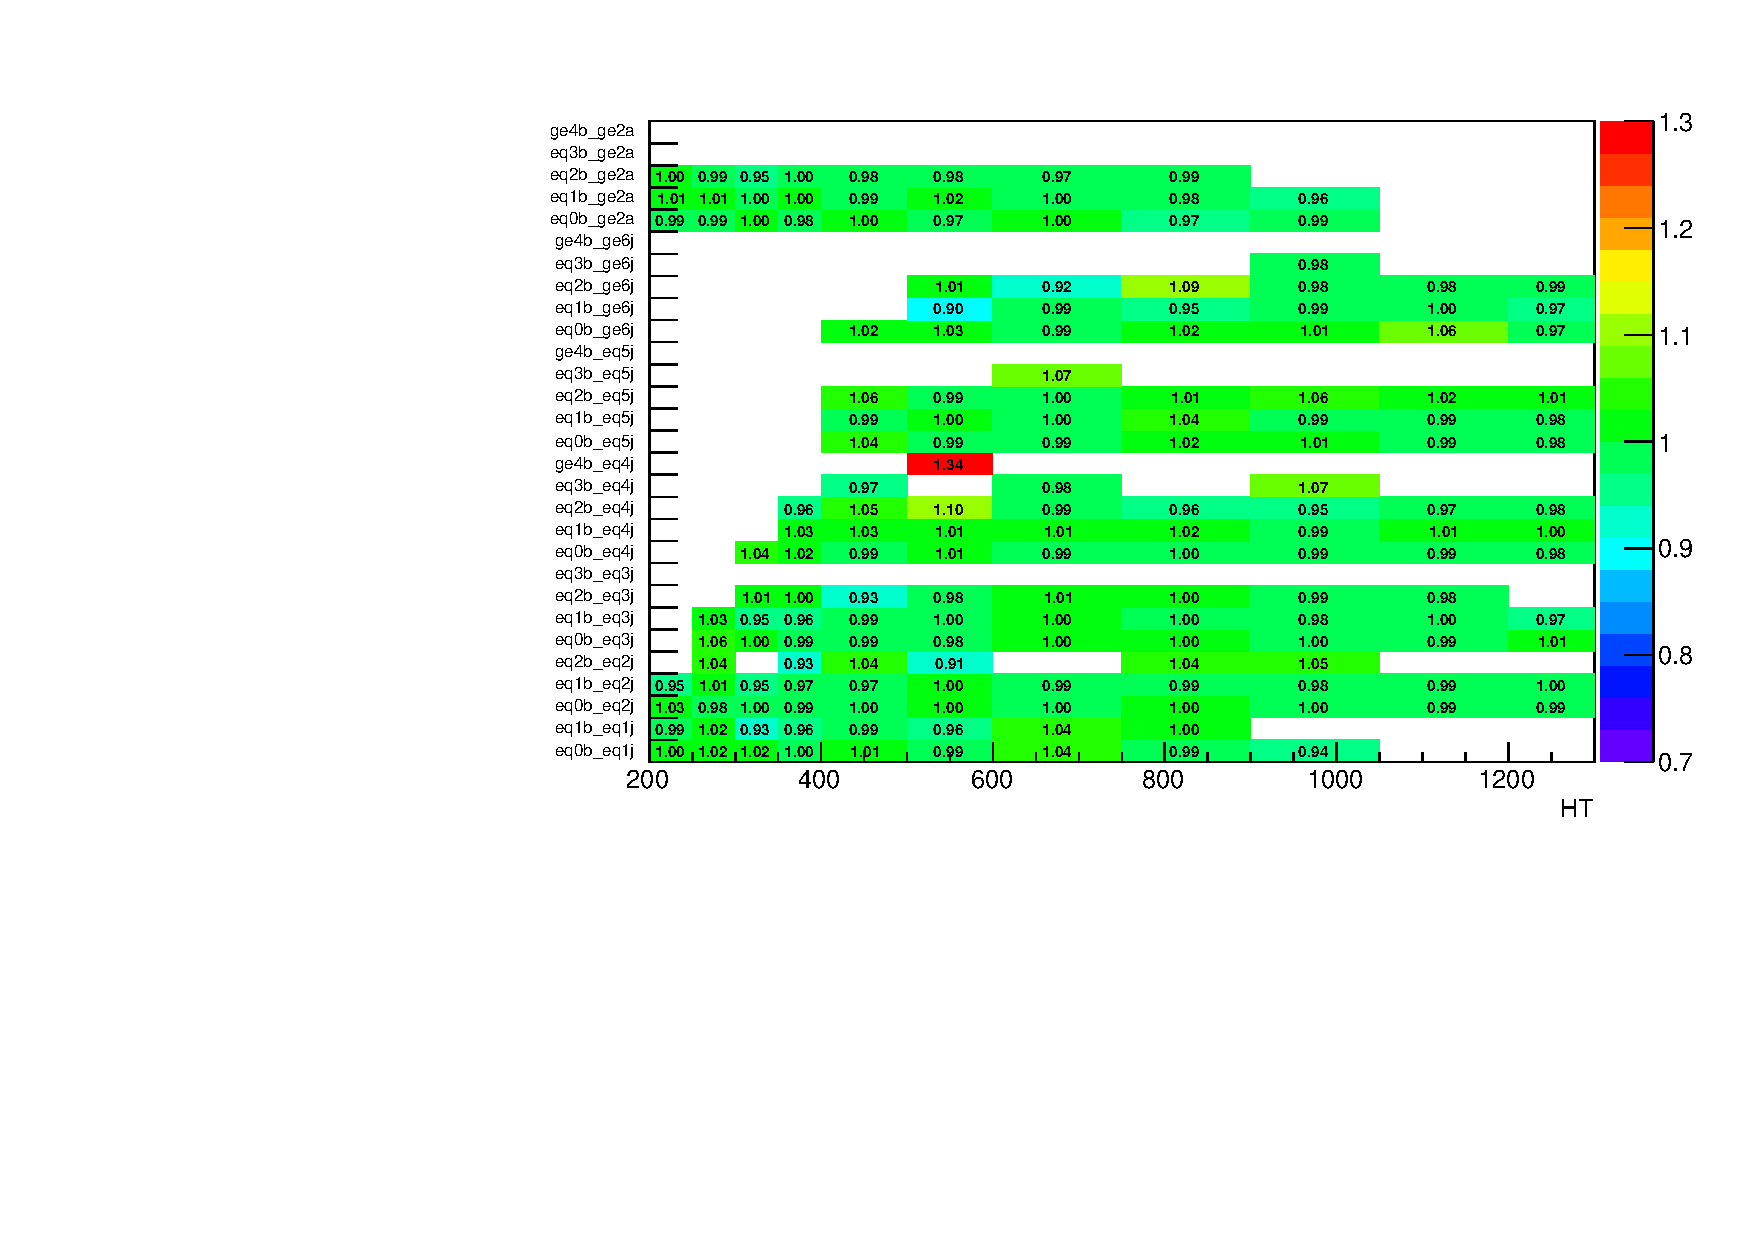
\includegraphics[width=0.5\textwidth]{figures/mcSystematics36p4fb/Zinv/mumu/ratiotfh_ht_mht_allpuWeight_Down.pdf}
  }\\

  \caption{\label{fig:tfSyst_pu_mumuToZinv} The relative change in the
  $\mmj \rightarrow (\znunu)$ transfer
  factors when varying PU weight in MC within its uncertainties, as a function of \scalht and jet category. 
  Variations corresponding to $+1\sigma$ ($-1\sigma$) are shown in the left (right) figure. 
  }
\end{figure}

\begin{figure}[!h]
  \centering
  \subfigure[PU weight up variation]{
    \includegraphics[width=0.5\textwidth]{figures/mcSystematics36p4fb/Zinv/gj/ratiotfh_ht_mht_allpuWeight_Up.pdf}
  } ~~
  \subfigure[PU weight down variation]{
    \includegraphics[width=0.5\textwidth]{figures/mcSystematics36p4fb/Zinv/gj/ratiotfh_ht_mht_allpuWeight_Down.pdf}
  }\\

  \caption{\label{fig:tfSyst_pu_gjToZinv} The relative change in the
  $\gj \rightarrow (\znunu)$ transfer
  factors when varying PU weight in MC within its uncertainties, as a function of \scalht and jet category. 
  Variations corresponding to $+1\sigma$ ($-1\sigma$) are shown in the left (right) figure. 
  }
\end{figure}

\begin{figure}[!h]
  \centering
  \subfigure[PU weight up variation]{
    \includegraphics[width=0.5\textwidth]{figures/mcSystematics36p4fb/Ttw/mu/ratiotfh_ht_mht_allpuWeight_Up.pdf}
  } ~~
  \subfigure[PU weight down variation]{
    \includegraphics[width=0.5\textwidth]{figures/mcSystematics36p4fb/Ttw/mu/ratiotfh_ht_mht_allpuWeight_Down.pdf}
  }\\

  \caption{\label{fig:tfSyst_pu_muToTtw} The relative change in the $\mj \rightarrow \mathrm{tt+W}$ transfer
  factors when varying PU weight in MC within its uncertainties, as a function of \scalht and jet category. 
  Variations corresponding to $+1\sigma$ ($-1\sigma$) are shown in the left (right) figure. 
  }
\end{figure}
